%如果需要稳定版,为documentclass添加可选参数stable
%如果需要暗色版,为documentclass添加可选参数dark
%不知道为什么,这个文档删除所有辅助文件后开始编译,需要连续编译11次才能够得到正确的结果;
%可以尝试把辅助文件也放进来,这样应该只要编译1次
\documentclass[dark]{Physics_H_Notes}
% 调整 headheight 和 topmargin
\setlength{\headheight}{12.67163pt}
\addtolength{\topmargin}{-0.67163pt}
\usepackage{upgreek}
\usepackage{tikzit}
\usepackage{cancel}
\usepackage{pgfplots}
\usepackage{tikz-3dplot}
\usepackage{lmodern}
\pgfplotsset{compat=newest}
\usepgfplotslibrary{fillbetween}
\input{arrow.tikzstyles}
\usetikzlibrary{3d,calc,positioning, shapes.geometric,decorations.fractals,arrows,intersections,decorations.text,shapes}
%这里也是,如果把上述内容改成\RequirePackage{package}再放入模板,会导致奇怪的识别错误
\begin{document}

%\definecolor{softblue}{rgb}{0.92,0.95,0.99}
\thispagestyle{empty}
\if@physicsHNotes@dark
	\newcommand{\apart}[1]%
	{
		\newpage
		\thispagestyle{empty}
		\stepcounter{apart}%
		\addcontentsline{toc}{chapter}{\large #1}%
		\begin{tikzpicture}[overlay,remember picture,font=\sffamily\bfseries]
			\fill[fill=backgroundcolor] (current page.south west) rectangle (current page.north east);
			
			\draw[ultra thick,gray4,name path=big arc] ([xshift=-2mm]current page.north) arc(150:285:11)
			coordinate[pos=0.225] (x0);
			\begin{scope}
				\clip ([xshift=-2mm]current page.north) arc(150:285:11) --(current page.north
				east);
				\fill[gray2!95!plaincyan] ([xshift=4.55cm]x0) circle (4.55);
				\fill[gray3!95!plaincyan] ([xshift=3.4cm]x0) circle (3.4);
				\fill[gray4!95!plaincyan] ([xshift=2.25cm]x0) circle (2.25);
				\draw[ultra thick,gray5!90!plaincyan] (x0) arc(-90:30:6.5);
				\draw[ultra thick,gray5!90!plaincyan] (x0) arc(90:-30:8.75);
				\draw[ultra thick,gray5!90!plaincyan,name path=arc1] (x0) arc(90:-90:4.675);
				\draw[ultra thick,gray5!90!plaincyan] (x0) arc(90:-90:2.875);
				\path[name intersections={of=big arc and arc1,by=x1}];
				\draw[ultra thick,gray5!90!plaincyan,name path=arc2] (x1) arc(135:-20:4.75);
				\draw[ultra thick,gray5!90!plaincyan] (x1) arc(135:-20:8.75);
				\path[name intersections={of=big arc and arc2,by={aux,x2}}];
				\draw[ultra thick,gray5!90!plaincyan] (x2) arc(180:50:2.25);
			\end{scope}
			\path[decoration={text along path,text color=textcolor,
				raise = -2.8ex,
				text  along path,
				text = {|\sffamily\bfseries|},
				text align = center,
			},
			decorate
			] ([xshift=-2mm]current page.north) arc(150:245:11);
			%
			\begin{scope}
				\path[clip,postaction={fill=gray2}]
				([xshift=2cm,yshift=-9.5cm]current page.center) rectangle ++ (4.2,7.7);
				\draw[ultra thick,gray4!80!plaincyan] ([xshift=-1.5cm,yshift=-9.5cm]current page.center)
				arc(180:0:2);
				\draw[ultra thick,gray4!80!plaincyan] ([xshift=0.5cm,yshift=-9.5cm]current page.center)
				arc(180:0:2);
				\draw[ultra thick,gray4!80!plaincyan] ([xshift=2.5cm,yshift=-9.5cm]current page.center)
				arc(180:0:2);
				\draw[ultra thick,gray4!80!plaincyan] ([xshift=4.5cm,yshift=-9.5cm]current page.center)
				arc(180:0:2);
				\fill[gray!50] ([xshift=2.5cm,yshift=-9.5cm]current page.center) +(60:2) circle(1.5mm);
				\node[text=textcolor!50!plaincyan] at ([xshift=4.7cm,yshift=-6.7cm]current page.center) {\LARGE \hspace*{-3.9em}G.P.A};
			\end{scope}
			%
			\fill[gray3] ([xshift=2cm,yshift=-9.5cm]current page.center) rectangle ++ (-13.7,7.7);
			\fill[backgroundcolor!90]([xshift=-2cm,yshift=-7.3cm]current page.center) rectangle ++ (-9.7,3);
			\node[text=textcolor!60!plaincyan,anchor=west,scale=4,inner sep=0pt] at
			([xshift=-10.55cm,yshift=-5.8cm]current page.center) {\ \,#1};
			\fill[gray4!80!plaincyan] ([xshift=-2cm,yshift=-7.3cm]current page.center) -- ([xshift=-2cm,yshift=-4.3cm]current page.center) -- ([xshift=-1cm,yshift=-5.8cm]current page.center) -- cycle;
		\end{tikzpicture}
	}
	\tikzset{pics/.cd,
		triple circle/.style={code={
				\fill[gray2] (4,0) circle (4);
				\fill[gray4] (3,0) circle (3);
				\fill[gray6] (2,0) circle (2);
	}}}
	\begin{tikzpicture}[overlay,remember picture]
		\fill[backgroundcolor] (current page.north west) rectangle (current page.south east); 
		\draw[gray] ([xshift=-1cm]current page.north) 
		-- node[midway, above, sloped, font=\LARGE, text=white] {$\displaystyle E=\gamma mc^2$}
		++ (-60:9) pic[rotate=90-60,scale=0.7] {triple circle};
		\draw[gray] (current page.north west) 
		-- node[midway, above, sloped, font=\LARGE, text=white] {$\displaystyle x'=\gamma\left(x-\beta ct\right)\qquad\qquad$}
		node[midway, below, sloped, font=\LARGE, text=white] {$\qquad\qquad\displaystyle ct'=\gamma\left(ct-\beta x\right)$}
		++ (-40:20) pic[rotate=90-40,scale=0.3] {triple circle};
		\draw[gray] ([yshift=-11cm]current page.north east) 
		-- node[midway, above, sloped, font=\LARGE, text=white] {$\displaystyle \vec{F}=m\vec{a}$}
		++ (-110:15) coordinate (endPoint) pic[rotate=90-110,scale=0.8] {triple circle};
		\node[above right=12cm and 2cm of current page.south west,font=\Huge\itshape,white] (H)
		{\underline{普通物理の超绝援助}};
		\node[below=1mm of H.south west,anchor=north west,font=\bfseries\LARGE,color=textcolor]{\ General Physics Assistance};
		\node[below=1.4cm of H.south west,anchor=north west,font=\itshape\LARGE,color=textcolor]{\ 混合普物{\bfseries\normalfont(H)}笔记小组\,\raisebox{0.2ex}{\tikz{\draw(0.15,0.15)circle(0.15);
					\draw(0.15,0.15)circle(0.1);}} 著};
		\node[above right=9cm and 12cm of current page.south west] (PPP) {};
		\node[right = 1mm of current page.south west] (PPL) {};
		\node[right = 2mm of current page.south west] (PPR) {};
		\draw[gray, thick] (current page.south west) 
		to[out=20, in=180] (PPP);
		\draw[gray, thick] (PPL) 
		to[out=20, in=180] (PPP);
		\draw[gray, thick] (PPR) 
		to[out=16, in=180] (PPP);
	\end{tikzpicture}
	%暗色版封面参考https://www.latexstudio.net/index/details/index/mid/3310
\else
	\newcommand{\apart}[1]%
	{
		\newpage
		\thispagestyle{empty}
		\stepcounter{apart}%
		\addcontentsline{toc}{chapter}{\large #1}%
		\begin{tikzpicture}[overlay,remember picture,font=\sffamily\bfseries]
			\fill[fill=thisgreen!2!thiswhite] (current page.south west) rectangle (current page.north east);
			
			\draw[ultra thick,c4,name path=big arc] ([xshift=-2mm]current page.north) arc(150:285:11)
			coordinate[pos=0.225] (x0);
			\begin{scope}
				\clip ([xshift=-2mm]current page.north) arc(150:285:11) --(current page.north
				east);
				\fill[c4!50,opacity=0.25] ([xshift=4.55cm]x0) circle (4.55);
				\fill[c4!50,opacity=0.25] ([xshift=3.4cm]x0) circle (3.4);
				\fill[c4!50,opacity=0.25] ([xshift=2.25cm]x0) circle (2.25);
				\draw[ultra thick,c4!50] (x0) arc(-90:30:6.5);
				\draw[ultra thick,c4] (x0) arc(90:-30:8.75);
				\draw[ultra thick,c4!50,name path=arc1] (x0) arc(90:-90:4.675);
				\draw[ultra thick,c4!50] (x0) arc(90:-90:2.875);
				\path[name intersections={of=big arc and arc1,by=x1}];
				\draw[ultra thick,c4,name path=arc2] (x1) arc(135:-20:4.75);
				\draw[ultra thick,c4!50] (x1) arc(135:-20:8.75);
				\path[name intersections={of=big arc and arc2,by={aux,x2}}];
				\draw[ultra thick,c4!50] (x2) arc(180:50:2.25);
			\end{scope}
			\path[decoration={text along path,text color=c4,
				raise = -2.8ex,
				text  along path,
				text = {|\sffamily\bfseries|},
				text align = center,
			},
			decorate
			] ([xshift=-2mm]current page.north) arc(150:245:11);
			%
			\begin{scope}
				\path[clip,postaction={fill=thisyellow!10!thiswhite}]
				([xshift=2cm,yshift=-9.5cm]current page.center) rectangle ++ (4.2,7.7);
				\draw[ultra thick,plaincyan] ([xshift=-1.5cm,yshift=-9.5cm]current page.center)
				arc(180:0:2);
				\draw[ultra thick,plaincyan] ([xshift=0.5cm,yshift=-9.5cm]current page.center)
				arc(180:0:2);
				\draw[ultra thick,plaincyan] ([xshift=2.5cm,yshift=-9.5cm]current page.center)
				arc(180:0:2);
				\draw[ultra thick,plaincyan] ([xshift=4.5cm,yshift=-9.5cm]current page.center)
				arc(180:0:2);
				\fill[thisred!20!thiswhite] ([xshift=2.5cm,yshift=-9.5cm]current page.center) +(60:2) circle(1.5mm);
				\node[text=c5!80!thisblack] at ([xshift=4.7cm,yshift=-6.7cm]current page.center) {\LARGE \hspace*{-3.9em}G.P.A};
			\end{scope}
			%
			\fill[thisred!5!thiswhite] ([xshift=2cm,yshift=-9.5cm]current page.center) rectangle ++ (-13.7,7.7);
			\fill[thisred!10!thiswhite]([xshift=-2cm,yshift=-7.3cm]current page.center) rectangle ++ (-9.7,3);
			\node[text=thisblack!60!thiswhite,anchor=west,scale=4,inner sep=0pt] at
			([xshift=-10.55cm,yshift=-5.8cm]current page.center) {\ \,#1};
			\fill[orangepink!60!thiswhite] ([xshift=-2cm,yshift=-7.3cm]current page.center) -- ([xshift=-2cm,yshift=-4.3cm]current page.center) -- ([xshift=-1cm,yshift=-5.8cm]current page.center) -- cycle;
		\end{tikzpicture}
	}
	\begin{tikzpicture}[remember picture,overlay,shorten >= -10pt]
		\fill[thisgreen!2!thiswhite] (current page.south west) rectangle (current page.north east);
		
		\coordinate (B1) at ([xshift=-8pt,yshift=-400pt]current page.north west);
		\coordinate (B2) at ([xshift=-8pt,yshift=-125pt]current page.north west);
		\coordinate (B3) at ([xshift=-50, yshift=-475pt]current page.north west);
		\coordinate (B4) at ([xshift=10pt,yshift=300pt]current page.south east);
		\coordinate (B5) at ([xshift=10pt,yshift=455pt]current page.south east);
		\coordinate (B6) at ([xshift=-300pt,yshift=-15pt]current page.south east);
		\coordinate (B7) at ([xshift=0pt,yshift=80pt]current page.south east);
		
		\begin{scope}[decoration=Koch snowflake]
			\draw (B3)  ++(43:7)coordinate(C3)  ++(123:7)coordinate(D3);
			
			\draw[titlepagecolor!20,line width=2pt,fill = thisred!5!thiswhite]
			decorate{decorate{decorate{decorate{(D3) -- (C3) -- (B3)}}}};
			
			\draw (B7)  ++(140:8)coordinate(C7)  ++(-175:8)coordinate(D7);
			
			\draw[titlepagecolor!30,line width=2pt,]
			decorate{decorate{decorate{decorate{(D7) -- (C7) -- (B7)}}}};
			
			\draw (B6) ++(100:10) coordinate(C6)  ;
			
			\draw[titlepagecolor!80,line width=1pt,fill = thisyellow!10!thiswhite]
			decorate{decorate{decorate{decorate{(current page.south west) -- (B1) -- (C6) --
							(B6)}}}} -- cycle ;
			
			\draw (B2)  ++(65:3) coordinate(C2)  ++(110:3) coordinate(D2);
			
			\draw[titlepagecolor!40,line width=1pt,]
			decorate{decorate{decorate{decorate{(D2) -- (C2) -- (B2)}}}};
			
			\draw (B2) ++(65:9)coordinate(E2);
			
			\draw[titlepagecolor!50,line width=1pt,]
			decorate{decorate{decorate{decorate{(E2) -- (B2)}}}};
			
			\draw[titlepagecolor!30,line width=3pt,rounded corners=6pt,fill=thiscyan!5!thiswhite]
			(B5) -- ++(135:2) -- ++(45:2);
			
			\draw[titlepagecolor!60,line width=4pt,rounded corners=6pt,fill=thiscyan!5!thiswhite]
			(B4) -- ++(135:5) -- ++(45:5);
		\end{scope}
		\node [xslant=0.2, scale = 3.1, anchor = north east,inner xsep = 0pt, ](author) at ([shift={(-0.1\paperwidth,0.35\paperheight)}]current page.east) {普\,通\,物\,理\,の\,超\,绝\,援\,助
		};
		
		\draw[line width=3pt] (author.south west) -- (author.south east);
		
		\node [scale = 3, anchor = north east, inner xsep = 0pt, ] at ([shift={(-0.1\paperwidth,0.24\paperheight)}]current page.east) {General Physics Assistance};
		
		\node [scale = 2, anchor = north east,inner xsep = 0pt, ] at ([shift={(-0.1\paperwidth,0.17\paperheight)}]current page.east) {混合普物(H)笔记小组\,\raisebox{-0.2ex}{\tikz{\draw(0.15,0.15)circle(0.15);
					\draw(0.15,0.15)circle(0.1);}}  \color{textcolor} 著};
	\end{tikzpicture}%
	
\fi
	
	\setcounter{page}{0}

\tableofcontents
\frontmatter
	\chapter{前言}
	在普物(H)的学习中,深感几个问题:
	\begin{Itemize}
		\item 英文好难,不想看ppt
		\item 老师讲得好抽象(我的问题,老师其实讲得很好了),听不懂
		\item 作业好烦,看不懂也找不到答案
		\item 小测好杂,内容好广
		\item 资料好少,复习好难
		\item 考试好可怕,还要读英文题目
	\end{Itemize}
	
	因此,我产生了一个念头:编写一份中英混搭的普物资料,把ppt和其它教科书全都迭代掉。这个想法可能有些大胆,但我依旧相信,我们可以做到。
	
	感谢普物H笔记计划的所有人\footnote{此处无先后顺序:陈锦浩,倪晟翔,陈若轩,刘远鉴,薛宇航,杨宏毅。},感谢大家的热情加入与支持。
	
	另外,感谢学长薛宇航及其朋友提供的普物笔记,没有他们提供的资料,这份文档的出生将会走更长更长的路。
	
	该笔记的内容基本基于2023学年春夏学期路欣老师的ppt,不保证之后普物(H)教学内容是否有所调整,请使用者自行斟酌。另外,习题部分也取自2023学年春夏学期的课后作业与小测,并对部分题目做了改编。
	
	本书中用到的图片,如果是非矢量图的,且未说明出处的,则来自ppt;其它非矢量图则都注明了出处;矢量图均使用tikz绘制。
	\chapter{约定}
	不要跳过一本书的约定,因为它能帮助你更好地阅读学习。
	
	本书约定如下:
	\setcounter{chapter}{-1}
	\refstepcounter{chapter}
	
	\begin{description}
		\item[语言风格]中英混搭。可能一个中英混搭的文档看起来不伦不类,但我希望它能让还没那么习惯英文的学生能更好地度过这一段过渡期。本文档内,\textbf{解释说明}的语句将采用\textbf{中文},而对于\textbf{问题的叙述},以及一些\textbf{关键词},将采用\textbf{英文},以保证大家的英语阅读思维能得到培养,不至于面对作业题与考试题束手无措。
		\item[交互图层] 很多关键词往往头一次见不是那么容易认得,因此,本文档提供交互图层:我们默认,当文字的颜色显示为{\color{plaincyan}青色}时,它将是可以交互的(这个除外),读者可以通过在PDF阅读器中打开并用鼠标点击的方式切换它的中英文显示。当然,一些并非关键词,但初见可能不认识的词,也会用该方式处理,便于读者查找中文意思。
		
		如果需要实现交互功能,可以选择Adobe Reader,Foxit Reader或Okular作为你的pdf阅读器,其中Adobe Reader,Foxit Reader收费\footnote{Foxit Reader在浙大正版软件平台中可以下载。},Okular开源。相对而言,前两者功能更强大,Okular则更简洁,轻便\footnote{这是对于其支持可交互图层渲染和批注的功能而言的,600M的大小比之3G的Foxit Reader当然算轻便,但和Sumatra那种完全旨在阅读的pdf阅读器来比当然算不了轻便。}。如果只有阅读和批注需要,Okular会是很好的选择\footnote{需要注意的是,右键打开含中文目录下的pdf文件时,Okular会出现显示错误,建议在Okular内打开文件,或者将pdf文件统一放在英文目录下管理。}。
		
		使用其它pdf阅读器时,为了防止阅读器报错,请选择本书的稳定版。稳定版会直接显示英文与中文,不再支持交互功能。
		
		\item[超链接]为了便于阅读,在文档中将出现许多的超链接。我们默认,当文字的颜色显示为{\color{blue}蓝色}时(这个也除外),它将可以作为超链接被点击。
		\item[跳转卡片]很多理科书目的前后引用在实际阅读中其实是一件麻烦的事情,本书将提供可以反向跳转的的超链接跳转卡片(如右)\labelroot{frontmatter:ref},读者可以通过在PDF阅读器中打开并用鼠标点击的方式点击跳转(\refleaftext{frontmatter:ref})。
		\item[*标记]普物\Romannumeral{1}中的部分内容较为困难,在实际考核中较少涉及。本书中部分内容用*标记,表示这些内容只需了解即可,不必掌握证明。
		\item [矢量与标量]本书中,不加粗的符号(如$v$)表示标量或取矢量的大小;加粗的符号(如$\vec{v}$)则表示矢量。
		\item [建议的阅读方式] 本书因为叙述要求,在内容顺序上与课堂可能有一定出入。如果决定使用本书学习普物(H),请确保学习的连续性,不要碎片式学习,以免在写作业时遇到困难。
		
		对于初学者,建议兼顾笔记的正文部分和证明部分;若是补天选手,如无特别说明,阅读正文部分即可。本书的习题部分都有详细的解答,可以自行练习。
	\end{description}

\mainmatter
\apart{正文部分}
\chapter[测量]{\itr{Measurement}{测量}}
本章节内容较为简单,一般相关题目会出现在日常上课的课后小测与作业内,大型考试基本不涉及。重点是掌握物理学的基本单位,以及利用国际单位制以及相关比例关系推导特殊物理量的单位表达式与可能的公式表达式。
\section[单位与量纲]{\itr{Unit \& Dimension}{单位与量纲}}
\begin{Itemize}
    \item \itr{Basic Quantity}{基本量}\ \eg Length($L$), Mass($M$), Time($T$)\\
    在自然世界中,我们会用各种物理量来描述物质的性质。就像在平面几何中我们可以基于几大公理推出各种定理,在物理中,我们也可以规定一些“基本的量”,使得所有的物理量可以由这些量导出。自然地,我们就称呼这些量为基本量。
    \item \itr{Unit}{单位}在规定好一些物理量之后,我们会想办法去度量它们。既出于定量测量的要求,又出于减少物理公式参数的考量,人们定义了各种各样的单位。
    \begin{itemize}
        \item \itr{SI Units}{国际单位制单位}\mgnote{SI $\Leftrightarrow$ International System of Units}\ \eg meter(m), kilogram(kg), second(s)
        \item \itr{Non SI Units}{非国际单位制单位}\ \eg mm, $\upmu$m, g\\
              \En{If you \itr{convert}{转化} everything to the basic SI units, you can \itr{omit}{省略} them during the calculation, but remember to put back the correct units at the end.}\\
              事实上,可以在计算过程中省略的约定也算是国际单位制存在的意义之一(\dove :大概吧)。
    \end{itemize}
    \item \itr{Dimension}{量纲}\ 一个物理量的量纲指的是这个物理量关于基本量的导出式。

    \eg 速度的量纲可以表示为[$v$]=$\dfrac{L}{T}$

    \item \itr{Dimension Analysis}{量纲分析}\ 量纲分析是检验物理公式正确性的好方法。简而言之,你可以简单地通过分析一个物理等式左右两边的量纲是否一致来初步判断这个等式可不可能成立。当然,量纲分析也可以作为导出实验公式大方向的一个指导,又或者……是你忘记了公式中的某一个物理量时尝试硬添物理量时的救命稻草。
\end{Itemize}
\section[数据处理]{\itr{Data Processing}{数据处理}}
这部分普通物理学实验\Romannumeral{1}\footnote{说到这里,\dove 还编写了一个用于普物实验数据处理的软件,链接为 \url{https://github.com/CrazySpottedDove/Lab-Assistance.git},如有需要,可以自行下载。}会详细说明并实际计算运用,非常抱歉,此处略去。
\section{课后习题:测量}

\begin{example}[量纲分析---\refleaftext{solution1.1}]
    The \itr{displacement}{位移} of a particle moving under \itr{uniform
        acceleration}{匀加速度} is some function of the \itr{elapsed time}{经历的时间} and
    the acceleration. Suppose we write this displacement
    $s=ka^mt^n$,where A is a \itr{dimensionless constant}{无量纲常数}. \\
    (1)Show by
    dimensional analysis that this expression is satisfied if
    $m = 1$ and $n = 2$. \\
    (2)Can this analysis give the value of A?
\end{example}




\chapter[质点运动学与动力学基础]{\itr{Fundamentals of particle kinematics and dynamics}{质点运动学与动力学基础}\mgnote*{\raggedleft 作者:23级-刘远鉴}}
\textbf{质点运动},即一个理想化的、质量集中于单一点的物体的运动。尽管现实世界中的物体都有一定的尺寸和形状,但通过将其简化为质点,我们可以更容易地分析和描述它们的运动特性。质点运动学就是研究质点运动的学科。它不关心引起运动的力,而是专注于描述运动本身:如位置、速度、加速度等随时间变化的规律。通过掌握这些基础的运动学概念和方程式,我们可以更好地理解和预测各种自然现象和工程应用中的运动行为。

相信大家在高中的时候都和质点运动学打过交道,那么大学的质点运动学和高中的又有什么不同呢?简而言之,就是加入了微积分这个强大的工具。

了解了运动学相关的知识后,我们将研究学习引起运动的力及其作用,包括功、能、动量等概念,也就是动力学的内容。
\section[一维运动]{\itr{Motion in 1D}{一维运动}}
讲质点运动,首先从一维的运动说起。
\subsection[质点运动学的基本概念]{\itr{Basic Concepts of Particle Kinematics}{质点运动学的基本概念}}
相信大家在高中时候以及对质点运动学的基本概念比较了解了,不多赘述,汇总如下\footnote{此时,我们还没有引入向量的观点,因此这里的符号全都是标量形式。}:
\begin{Itemize}
       \item \itr{Displacement}{位移} $\Delta x=x_{f} -x_{i}$
       \item \itr{Average Velocity}{平均速度} $v_{avg} =\dfrac{x_{f}-x_{i}  }{t_{f}-t_{i}  } $
       \item \itr{Average Speed}{平均速率} $s_{avg} =\dfrac{total\ distance}{total\ time} $ 
       \item \itr{Instantaneous Velocity}{瞬时速度} $\displaystyle v=\lim_{\Delta t \to 0} \frac{\Delta x}{\Delta t} =\frac{\dif  x}{\dif  t} $
\end{Itemize}
\begin{Itemize}
       \item \itr{Instantaneous Speed}{瞬时速率} $\left | v \right | >0$ ,即瞬时速度的大小
       \item \itr{Average Acceleration}{平均加速度} $a_{avg} =\dfrac{v_{f}-v_{i}  }{t_{f}-t_{i}  } $
       \item \itr{Instantaneous Acceleration}{瞬时加速度} $\displaystyle a=\lim_{\Delta t \to 0} \frac{\Delta v}{\Delta t} =\frac{\dif  v}{\dif  t} = \frac{\dif ^2x}{\dif  t^2} $
\end{Itemize}
注意这里的下标,avg代表average,i代表initial,f代表final。做题的时候自己写上这样的下标也是很清晰的。
\subsection[质点运动学有关的计算]{\itr{Calculations Related to Particle Kinematics}{质点运动学有关的计算}}
\eg 已知位移与时间的关系$x=At^{n} $,可求得t时刻的瞬时速度为$v=\dfrac{\dif  x}{\dif  t} =Ant^{n-1} $。进一步也可以求得t时刻的瞬时加速度,留给读者。

那么,上面例子中的过程能否反向进行呢?知道瞬时加速度与时间的关系,能否推出速度、位移与时间的关系呢?下面是一个例子:

已知加速度关于时间的表达式为$a=a(t)$,初始时刻为$t_{i} $,那么由于$a=\dfrac{\dif  v}{\dif  t}$,形式上移项可得 $\dif  v=a(t)\dif  t$。等式两边从初始时刻$t_{i}$到当前时刻$t$积分,可得\mgnote{左右两边的常数项合并了。}
\[v(t)=\int_{t_{i}}^{t}a(t') \dif  t'+C_{1}\]
代入$t=t_{i}$,可求得$C_{i}=v_{i}$。如此,我们便得到了速度关于时间的表达式
\[v(t)=\int_{t_{i}}^{t}a(t')\dif  t'+v_{i}\]

在上面计算的基础上,进一步可以求得位移关于时间的表达式(已知初始位移为$x_{i}$):
\begin{equation}
    \begin{aligned}
    x(t)&=\int_{t_{i}}^{t}v(t')\dif  t'+x_{i}\\
    & =\int_{t_{i}}^{t} \dif  t'\left[\int_{t_{i}}^{t'}a(t'')\dif  t''+v_{i}\right]+x_{i}\\
    & =x_{i}+(t-t_{i})v_{i}+\int_{t_{i}}^{t}\dif  t'\int_{t_{i}}^{t'}\dif  t''a(t'')  
     \end{aligned}
    \nonumber
\end{equation}

至此,我们已经得到了相当具有普遍性的两个公式,尽管它们显得十分复杂。如果加速度是一个常数$a$,那么化简这两个公式,就可以得到大家高中时候倒背如流的几个公式:
\begin{equation}
    \begin{aligned}
    &v(t)=v_{i}+at\\
    &x(t)=x_{i}+v_{i}t+\frac{1}{2}at^{2}\\
    &x(t)-x_{i}= \frac{1}{2} (v_{i}+v_{f})t=\frac{v_{f}^{2}-v_{i}^{2}}{2a} 
    \end{aligned}
    \nonumber
\end{equation}

计算练习:已知$a(t)=at^{\alpha }$,其中$\alpha$是正的常数,$v_{i}$,$x_{i}$都是已知的,试求出$v(t)$,$x(t)$这两个表达式。
\section[高维的质点运动]{\itr{Motion in High Dimensions}{高维的质点运动}}
看起来很高大上的节标题,其实就是引入向量来更好地研究质点运动。

首先让我们来回忆一下,高中时期我们是怎么研究一个小球的平抛运动的。很自然地,我们一般会从竖直方向和水平方向两个方向来分解这个平抛运动,得到两个还算简单的表达式,并认为我们成功描述了这个平抛运动。

但是,如果大家尝试从水平和竖直两个方向去描述一个斜抛运动,或是在一个倾斜的坐标系下去描述一个平抛运动,就会发现,结果是一个带着三角函数的复杂式子。这仅仅只是对于二维的、一个质点的讨论。可以想象,用这种track each component的研究分量的方式讨论更高的维度或是更多的质点,会有更多的麻烦。
\ctikzfig{chapter2_without_vectors}
\begin{center}
	在倾斜的坐标系下描述平抛运动
\end{center}

那么,有什么方法能够让我们避开对于多个分量的繁琐讨论呢?没错,就是 \itr{vector}{向量}。
\subsection[向量]{\itr{Vector}{向量}}
\begin{Itemize}
	\item \itr{vector}{向量}: \En{A \itr{quantity}{量} that has both \itr{direction}{方向} and \itr{magnitude}{大小} and also obeys \itr{the laws of vector addition}{向量加法规律}\mgnote{我们假设读者已经知道向量加法规则,此略。}.}
\end{Itemize}

向量的常见表示方法:$\mathbf{a}$(boldface粗体表示)或者$\vec{a}$。本书中采用后者。

用向量来研究高维质点运动的好处:
\begin{Itemize}
    \item \itr{concise}{精确}:精确而简洁。
    \item \itr{independent of the choice of the coordinate axes}{与坐标系的选取无关}:用向量研究质点运动时,确定坐标系不再是必要的。
\end{Itemize}
虽然说向量与坐标系的选取无关,但我们常常在一个给定的坐标系下去描述一个向量。对于不同的坐标系及不同的\textbf{基底}(base),同一个向量的表示也是不一样的。
如何理解这句话呢?给大家看一个例子\labelroot{chapter2_vector_expression}:

首先,我们从最常见的\textbf{笛卡尔坐标系}(cartesian coordinate)说起。对于向量$\vec{r}$,高中的时候,我们会假设$\vec{r}=(x,y)$ ——其实这里我们省略了基的选取。更加严谨而普遍的表示方式应该是:设$\displaystyle\vec{r} =\left \{ \vec{e }_{1} ,\vec{e }_{2}  \right \} \binom{x}{y} =x\vec{e }_{1}+y\vec{e }_{2}$\footnote{这里的花括号其实就是矩阵的括号,用花括号是为了表示基底的更加清晰(但不严谨)的写法。大家可以将这个表达式理解为一个行向量和列向量的矩阵乘法(向量内积),这样更好记忆。但事实上$\left \{ \vec{e }_{1} ,\vec{e }_{2}  \right \}$应该是一个分块矩阵的表示,因为$\vec{e }_{1}$和$\vec{e }_{2}$本身也是列向量。}。
对于 \itr{Cartesian Coordinate}{笛卡尔坐标系},$\vec{e }_{1}$是$\displaystyle\binom{1}{0} $,$\displaystyle
\vec{e }_{2}$是$\displaystyle\binom{0}{1} $(也就是x轴,y轴方向的单位向量),代入上面假设的表达式,可以得到$\displaystyle\vec{r}=\binom{x}{y}  $。
\begin{center}
\begin{tikzpicture}[scale=0.8]

  \draw[->] (-3,0) -- (3,0) node[right] {$x$}; % x轴
  \draw[->] (0,-3) -- (0,3) node[above] {$y$}; % y轴

  \draw[->, thick, thisblue] (0,0) -- (1,0) node[midway, below] {$\vec{e}_1$}; % e1向量
  \draw[->, thick, thisred] (0,0) -- (0,1) node[midway, right] {$\vec{e}_2$}; % e2向量
\end{tikzpicture}

	\em 笛卡尔坐标系的基底

\end{center}

进一步,我们应当跳脱笛卡尔坐标系,去考量一些更加普遍的情况。在线性代数中,我们学习过线性空间和它的基。对于我们要考虑的n维空间,只要取n个\linebreak\itr{linearly independent}{线性无关} 的$\vec{e_{i} }$就可以了。这个时候,一个向量可能会表示成这个样子:
\[\vec{a} =\left \{ \vec{e_{1} } ,\vec{e_{2} } ,\ldots\vec{e_{n} }\right \} 
\begin{bmatrix}
  a_{1} \\
  a_{2} \\
  ...\\
  a_{n}
\end{bmatrix}\]

\subsection[向量与标量]{\itr{Vector versus Scalar}{向量vs标量}}
为了让大家更好地理解向量,这里区分一组概念:\itr{vertor}{向量} 和 \itr{scalar}{标量}。
\begin{Itemize}
	\item \itr{scalar}{标量} \En{A \itr{quantity}{量} having \itr{magnitude}{大小} but no \itr{direction}{方向} is a \itr{scalar}{标量}.}
\end{Itemize}
常见的标量:T(\itr{temperature}{温度}), m(\itr{mass}{质量}), s(\itr{speed}{速率})\mgnote{注意,向量的大小就是一个标量。}
\subsection[向量的大小与单位向量]{\itr{Magnitude and Unit Vector}{向量的大小与单位向量}}
向量$\vec{A}$的大小被表示为$A$或$\left | \vec{A} \right | $。说两个向量相等,等价于说两个向量大小相等,方向相同。

单位向量就是大小为1个单位的向量。
\begin{Itemize}
	\item \itr{unit vector}{单位向量} \En{A unit vector is a \itr{dimensionless}{无量纲的} vector having a magnitude of exactly 1.}
	\\
	注意,量纲的英文是dimension,题目中出现的时候要注意上下文语义。
\end{Itemize}

欲求一个向量同方向的单位向量,可取$\displaystyle\hat{\vec{r}} =\frac{\vec{r} }{\left | \vec{r} \right | } $。
\subsection[向量的运算]{\itr{Vector Algebra}{向量的运算}}
向量加法(vector addition),大家高中的时候都学过,共起点的时候使用平行四边形法则,首尾相连的时候使用三角形法则。

加法运算满足下面两个规律:
\begin{Itemize}
     \item \itr{Associaive law of addition}{加法结合律}:$\vec{A}+(\vec{B}+\vec{C})=(\vec{A}+\vec{B})+\vec{C}$
     \item \itr{Commutative law of addition}{加法交换律}:$\vec{A}+\vec{B}=\vec{B}+\vec{A}$
\end{Itemize}
这两个规律的证明,除了图像几何证明之外,还可以用上面我们提到的向量的表示方法\mgnote{见\refleaftext{chapter2_vector_expression}}来证明,推荐大家自己尝试一下。尝试之后可以发现,向量的加法交换律和结合律,都是基于实数的加法交换律和结合律。

一个向量$\vec{A}$的负向量(negative) $-\vec{A}$定义为与$\vec{A}$的向量和为$\vec{0}$(零向量)的向量,也就是与原向量等大反向的向量。

向量的减法(vector subtraction)可以用向量的加法与负向量定义:
\[\vec{A}-\vec{B}=\vec{A}+(-\vec{B})\]

在新的视角下,向量的数乘也可以这样理解($\alpha$是参与数乘的标量):
\[\alpha \vec{a}=\alpha \sum_{i=1}^{n}  a_{i} \vec{e }_{i} =\sum_{i=1}^{n} (\alpha a_{i} )\vec{e }_{i}\]         
          
向量的内积(scalar product)\labelroot{chapter2_scalar_product}:
\[\vec{a} \cdot\vec{b}=(\sum_{i}^{}a_{i}\vec{e}_{i}  )(\sum_{j}^{}b_{j}\vec{e}_{j}  ) =\sum_{i}^{}\sum_{j}^{}a_{i}b_{j}(\vec{e}_{i}\cdot\vec{e}_{j})  \]
特别的,对于 \itr{cartesian coordinate}{笛卡尔坐标系}\mgnote{这里拓展到多维情形。},有\mgnote{$\delta$念作delta。}
\[\vec{e}_{i}\cdot\vec{e}_{j}=\delta _{ij}=\begin{cases}
    1 & \text{ if } i=j \\
     0& \text{ if } i\ne j
   \end{cases}\]
于是有
\[\vec{a} \cdot \vec{b}=\sum_{i}^{} \sum_{j}^{} a_{i} b_{j} \delta _{ij} =\begin{bmatrix}
    a_1 & a_2 & \cdots & a_n
  \end{bmatrix}
  \begin{bmatrix}
    b_1 \\
    b_2 \\
    \vdots \\
    b_n
  \end{bmatrix}\]

向量内积满足下面几个基本律:
\begin{Itemize}
    \item \itr{Commutative Law}{交换律} 
    $\vec{a} \cdot \vec{b} = \vec{b} \cdot \vec{a}$
    \item \itr{Distributive Law}{分配律} 
    $\vec{a} \cdot (\vec{b} + \vec{c}) = \vec{a} \cdot \vec{b} + \vec{a} \cdot \vec{c}$
    \item \itr{Scalar Multiplication Property}{数乘律} 
    $k(\vec{a} \cdot \vec{b}) = (k\vec{a}) \cdot \vec{b} = \vec{a} \cdot (k\vec{b})$,其中 $k$ 是实数。
\end{Itemize}

向量的模长可以用内积表示:$r=\left | \vec{r} \right | =\sqrt{\vec{r}\cdot\vec{r}} $。

\subsection[极坐标]{\itr{Polar Coordinate}{极坐标}\labelroot[16pt]{chapter2_polar_coordinate}}
二维的情况: $\begin{cases}
    x=r\cos \theta \\
    y=r\sin \theta
   \end{cases}$
\begin{center}
\begin{tikzpicture}[scale=1]
    % 绘制坐标轴
    \draw[->] (0,0) -- (3,0) node[right] {$x$}; % x轴
    \draw[->] (0,0) -- (0,3) node[above] {$y$}; % y轴

    % 绘制极坐标点
    \draw[->, thick] (0,0) -- (1.5,1.5) node[above] {$P(r,\theta)$};
    \node[left] (0,0) {$O$};
    % 角度标记
    \draw[->] (0.5,0) arc (0:45:0.5) node[midway, right] {$\theta$};
    
    % r的长度标记
    \draw[dotted] (0,0) -- (1.5,1.5) node[midway, right] {$r$};
\end{tikzpicture}

\text{二维极坐标}
\end{center}

二维极坐标系的基本要素是极点和极轴,其中,极轴是一条从极点引出的有向轴。在上图中,极点即为$O$,而极轴则与$x$轴方向相同。我们用$(|\vec{r}|,\theta)$来表示一个点的位置。其中,$\vec{r}$表示以极点为起点,以被描述点为终点的向量,称为极径矢量;$\theta$则表示从极轴出发逆时针旋转到极径矢量的角度。可以发现,$\theta$并不唯一,我们一般取$2\pi$以内的角。

注意极坐标系同样也是有基底的,而且也是正交的。在极坐标中,特别定义$\hat{\vec{r}}$为$\vec{r}$增加方向的单位矢量,$\hat{\vec{\theta}}$为$\theta$增加方向的单位矢量,两者构成一对单位正交基。

\ctikzfig{chapter2_polar_coordinate_2d}
\begin{center}
	二维极坐标系的基底
\end{center}

三维的情况:$\begin{cases}
    x=r\sin\theta \cos\varphi \\
    y=r\sin\theta \sin\varphi \\
    z=r\cos\theta
   \end{cases}$
\begin{center}
	\resizebox{15em}{30ex}{
		\begin{tikzpicture}
			%draw the axes
			\draw[->] (0,0,0) -- (2.5,0,0) node[anchor=west]{$x$};
			\draw[->] (0,0,0) -- (0,2.5,0) node[anchor=west]{$z$};
			\draw[->] (0,0,0) -- (0,0,2.5) node[anchor=west]{$y$};
			%draw the top and bottom of the cube
			\draw[dotted,gray!50!thiswhite] (0,2,0) -- (2,2,0) -- (2,0,0);
			\draw[dotted,gray!50!thiswhite] (2,0,2) -- (0,0,2) -- (0,2,2) -- (2,2,2);
			
			%draw the edges of the cube
			%\draw[dashed,gray] (0,0,0) -- (0,0,2);
			\draw[dotted,gray!50!thiswhite] (0,2,0) -- (0,2,2);
			\draw[dashed,thisblack] (2,0,0) -- (2,0,2);
			\draw[dotted,gray!30!thiswhite] (2,2,0) -- (2,2,2);
			
			%  
			\draw[thick,thisblue!50!black,->] (0,0,0) -- (2,2,2) node[anchor=west,above=-14pt,right=-14pt]{$\boldsymbol{r}$};
			\draw[dashed,black] (0,0,0) -- (2,0,2);
			%\draw[dashed,black] (0,2,0) -- (2,2,2);
			\draw[dashed,black] (2,2,2) -- (2,0,2);
			
			% arcs
			%\coordinate (O) at (0,0,0);
			\tdplotdrawarc[<-,rotate around x=90,thisgreen!50!black]{(0,0,0)}{0.5}{0}{45}{above=-1pt,right=0pt,anchor=mid west}{$\varphi$};%\tdplotdrawarc[]{(O)}{r}{theta}{theta+Delta_theta}
			\tdplotdrawarc[<-,rotate around y=-45,thisred!80]{(0,0,0)}{0.5}{35.264}{90}{right=9pt,above=4pt,anchor=mid east}{$\theta$}
			\node[above=2pt, right=1pt,thisblack!70,scale=0.8] at (2,2,2) {$(x,y,z)$};
		\end{tikzpicture}
	}
	
	三维极坐标(来自 \url{https://www.latexstudio.net/index/details/index/mid/2316 })
\end{center}

\subsection[基变换]{\itr{Basis Transformation}{基变换}}
我们考虑一个简单的坐标系旋转的变换:
\ctikzfig{chapter2_basis_transformation}
\[\begin{cases}
	x'=OD+DF=x\cos\theta+y\sin\theta\\
	y'=PC-FC=y\cos\theta-x\sin\theta
\end{cases}\]

两个式子可以用一个矩阵乘法的式子表示:
\[\left [ x',y' \right ] =\left [ x,y \right ]\begin{bmatrix}
  \cos\theta &-\sin\theta \\
   \sin\theta&\cos\theta
 \end{bmatrix}\]

对于原坐标系中的一点$(x,y)$,只需要乘上基变换矩阵$\begin{bmatrix}
  \cos\theta &-\sin\theta \\
   \sin\theta&\cos\theta
 \end{bmatrix}$,就能得到该点在新坐标系下的坐标$(x',y')$。

 \subsection[质点运动的向量表示法]{\itr{Vector Representation of Particle Motion}{质点运动的向量表示}}
 无论是一维质点运动还是高维质点运动,都可以统一用向量来表示。
 \begin{Itemize}
  \item \itr{Position}{位置} $\vec{r}$
  \item \itr{Displacement}{位移} $\Delta\vec{r}=\vec{r}_{f}-\vec{r}_{i}$
  \item \itr{Average Velocity}{平均速度} $\vec{v}_{avg}=\dfrac{\Delta \vec{r}}{\Delta t}$
  \item \itr{Instantaneous Velocity}{瞬时速度} $\displaystyle\vec{v}=\lim_{\Delta t \to 0} \frac{\Delta \vec{r}}{\Delta t}=\frac{\dif \vec{r}}{\dif  t}$
  \item \itr{Average acceleration}{平均加速度} $\vec{a}_{avg}=\dfrac{\vec{v}_{f}-\vec{v}_{i}}{t_{f}-t_{i}}$
  \item \itr{Instantaneous acceleration}{瞬时加速度} $\displaystyle\vec{a}=\lim_{\Delta t \to 0}\frac{\Delta \vec{v}}{\Delta t}=\frac{\dif \vec{v}}{\dif  t}$
\end{Itemize}

而且向量表示也为我们对于基底以及分量的分析提供了便利:
\begin{equation}
  \begin{aligned}
    &\vec{r} =x\hat{\vec{i}}\mgnote{$\hat{\vec{i}}$的上标符号用于表示基底。} +y\hat{\vec{j}} +z\hat{\vec{k}} \\
\Longrightarrow &\vec{v}=\frac{\dif \vec{r}}{\dif  t}=\frac{\dif  x}{\dif  t}\hat{\vec{i}}+\frac{\dif  y}{\dif  t}\hat{\vec{j}}+\frac{\dif  z}{\dif  t}\hat{\vec{k}}=v_{x}\hat{\vec{i}}+v_{y}\hat{\vec{j}}+v_{z}\hat{\vec{k}}\\
   \end{aligned}
  \nonumber
\end{equation}

类似的,对于加速度也有:
\begin{equation}
  \begin{aligned}
   \vec{a}=a_{x}\hat{\vec{i}}+a_{y}\hat{\vec{j}}+a_{z}\hat{\vec{k}}
   \end{aligned}
  \nonumber
\end{equation}

\subsection[抛体运动]{\itr{Projectile Motion}{抛体运动}}
\begin{center}
  \begin{tikzpicture}[scale=1.5]

      % 轴
      \draw[->] (0,0) -- (4,0) node[right] {$x$};
      \draw[->] (0,0) -- (0,3) node[above] {$y$};
      
      % 斜抛轨迹
      \draw[thick, thisblue, domain=0:2.5] plot (\x, -\x^2+\x*2);

      % 初始速度矢量
      \draw[->, thick, thisred] (0,0) -- (1,2) node[right] {$\vec{v_0}$};

      % 角度标记
      \draw[->] (0,0) -- (0.5,0) arc (0:40:0.9) node[midway, right] {$\phi_0$};

      % 标注初始点
      \node at (0, -0.2) {O};

  \end{tikzpicture}
\end{center}

普遍的,对于一个匀加速运动,有$\vec{r}=\vec{r}_{0}+\vec{v}_{0}t+\dfrac{1}{2}\vec{a}t^{2}$。

\vspace*{0.4ex}
对于上图所示的简单的抛体运动,我们这样计算物体重新落到$x$轴上时,距离开始的时间和距离:
\begin{equation}
  \begin{aligned}
   \vec{r}_{f}&=s\hat{\vec{i}}+0\hat{\vec{j}}\\
   \Rightarrow\begin{pmatrix}
    s\\
    0
   \end{pmatrix}&=\begin{pmatrix}
                   v_{0}\cos\phi_{0}t\\
                   -v_{0}\sin\phi_{0}t 
                 \end{pmatrix}+\begin{pmatrix}
                                            0\\
                                            -\dfrac{1}{2}gt^{2}
                                          \end{pmatrix}\\
   \Longrightarrow t&=\frac{2v_{0}\sin\phi_{0}}{g}\\
   \Longrightarrow s&=\frac{v_{0}^{2}\sin2\phi_{0}}{g}
  \end{aligned}
  \nonumber
\end{equation}

再来看一个射击自由落体的靶子的例子:
\begin{center}
  \begin{tikzpicture}[scale=1.5]

      % 轴
      \draw[->] (0,0) -- (4,0) node[right] {$x$};
      \draw[->] (0,0) -- (0,3) node[above] {$y$};
      
      % 斜抛轨迹
      \draw[thick, thisblue, domain=0:2] plot (\x, -\x^2+\x*2);

      % 初始速度矢量
      \draw[->, thisblack] (0,0) -- (1,2) node[right] {T target};
      \draw[->, thick, thisred] (0,0) -- (0.5,1) node[left] {$\vec{v}_0$};
      \draw[->,thisblue] (1,2) -- (1,1) node[above right] {hit};
      % 角度标记
      \draw[->] (0,0) -- (0.5,0) arc (0:40:0.9) node[midway, right] {$\phi_0$};

      % 标注初始点
      \node at (0, -0.2) {O};

  \end{tikzpicture}
\end{center}

Q1:在靶子下落的一瞬间开枪,问枪应该瞄准哪里?

一个很巧妙的方法,就是进行一个坐标系变换,即考虑竖直向下以加速度$g$运动的非惯性参考系。在该参考系中,靶子是静止的,而枪的子弹不会下落而是作直线运动。那自然就应该直接瞄准靶子就行了。

Q2:子弹发射的最小速度是多少?

在上一问的参考系中,很容易得出子弹飞行的时间是$\dfrac{|OT|}{v_{0}}$。$OT$的长度是给定的,那么要求的最小速度,可以通过求最大飞行时间来得到。最大飞行时间是多少呢?很简单,就是在靶子要落地的瞬间才击中,这样时间最长,这个问题也就迎刃而解了。

当然,也可以不用坐标系的变换,直接这样计算:
\[\left\{
\begin{aligned}
  & \text{子弹位置:} \quad \vec{r}_{_P}=\vec{v}_{0}t - \frac{1}{2}gt^{2}\hat{\vec{j}} \\
  & \text{靶子位置:} \quad \vec{r}_{_T}=\left(|OT|\cos\phi_{0}\hat{\vec{i}} + |OT|\sin\phi_{0}\hat{\vec{j}}\right) - \frac{1}{2}gt^2\hat{\vec{j}}
\end{aligned}
\right.\]
加之$\vec{r}_{_P}=\vec{r}_{_T}$,即可解出要打中需要的角度和击中的时间。

\subsection[匀速圆周运动]{\itr{Uniform Circular Motion}{匀速圆周运动}}
下面,用我们用向量方法来研究一下匀速圆周运动的加速度表达式:

\vspace*{2ex}
\begin{minipage}{0.9\textwidth}
	\begin{minipage}{0.6\linewidth}
		\begin{center}
			\thisincludegraphics[width=0.7\textwidth]{chapter2_uniform circular motion}
			
			匀速圆周运动(本图出自\url{https://www.cnblogs.com/1024th/p/10744727.html})
		\end{center}
	\end{minipage}
	\quad
	\begin{minipage}{0.35\linewidth}
			\[\vec{a}=\lim_{\Delta t \to 0} \frac{\Delta \vec{v}}{\Delta t}\]
				由简单的几何关系可知,任何一点的加速度$\vec{a}$都垂直于切线方向,指向圆心。
	\end{minipage}
\end{minipage}
\vspace*{2ex}

确定方向后,再确定大小,即有:
\begin{equation}
  \begin{aligned}
         \left | \Delta \vec{v} \right |&=2v\sin\frac{\theta}{2} \\
    \Longrightarrow \left | \vec{a} \right |&=\lim_{\Delta t \to 0}  \frac{2v\sin\frac{\theta}{2}}{\Delta t}=\lim_{\Delta t \to 0}  \frac{2v\sin\frac{v\Delta t}{2r}}{\Delta t}=\frac{v^{2}}{r} \\
    \Longrightarrow \vec{a}&=-\frac{v^{2}}{r}\hat{\vec{r}}
  \end{aligned}
  \nonumber
\end{equation}

也可以用上极坐标来研究这个问题。之前提到过,极坐标也有一对正交基,如果将其理解为$x,y$轴正交基的旋转的话,就有如下表达式:

\[\left \{ \hat{\vec{r}},\hat{\vec{\theta}} \right \} =\left \{ \hat{\vec{i}},\hat{\vec{j}} \right \}\begin{pmatrix}
  \cos\theta & -\sin\theta\\
   \sin\theta& \cos\theta
 \end{pmatrix} \]
对称地,也有:
\[\left \{ \hat{\vec{i}},\hat{\vec{j}} \right \} =\left \{ \hat{\vec{r}},\hat{\vec{\theta}} \right \}\begin{pmatrix}
  \cos\theta & \sin\theta\\
  - \sin\theta& \cos\theta
 \end{pmatrix} \]

 如此可以推出
 \begin{equation}
  \begin{aligned}
      \frac{\dif \hat{\vec{r}}}{\dif t}&=\frac{\dif \cos\theta}{\dif t}\hat{\vec{i}}+\frac{\dif \sin\theta}{\dif t}\hat{\vec{j}}\\
         &=-\sin\theta\frac{\dif \theta}{\dif t}\hat{\vec{i}}+\cos\theta\frac{\dif \theta}{\dif t}\hat{\vec{j}}\\
&=-\sin\theta\frac{\dif \theta}{\dif t}(\cos\theta\hat{\vec{r}}-\sin\theta\hat{\vec{\theta}})+\cos\theta\frac{\dif \theta}{\dif t}(\sin\theta\hat{\vec{r}}+\cos\theta\hat{\vec{\theta}})\\
&=\frac{\dif \theta}{\dif t}\hat{\vec{\theta}}
  \end{aligned}
  \nonumber
\end{equation}

类似地\footnote{这要仔细想想,$\frac{\dif \theta}{\dif t}$是角速度的大小,但$\frac{\dif \hat{\vec{\theta}}}{\dif t}$却并不是角速度!目前我们讨论的暂时都是角速度的大小,至于角速度本身,将在第三章详细介绍。},也有
\[\displaystyle\frac{\dif \hat{\vec{\theta}}}{\dif t}=-\frac{\dif \theta}{\dif t}\hat{\vec{r}}\]

这两个式子和匀速圆周运动加速度有啥关系?别急,慢慢推导:
\begin{equation}
  \begin{aligned}
    &\vec{v}=\frac{\dif \vec{r}}{\dif t}=\frac{\dif {r\hat{\vec{r}}}}{\dif t}=r\frac{\dif \hat{\vec{r}}}{\dif t}=r\frac{\dif \theta}{\dif t}\hat{\vec{\theta}}=r\omega \hat{\vec{\theta}}\\
\Longrightarrow &\vec{a}=\frac{\dif \vec{v}}{\dif t}=r\omega\frac{\dif \hat{\vec{\theta}}}{\dif t}=r\omega(-\frac{\dif \theta}{\dif t}\hat{\vec{r}} )=-\omega^{2}r\hat{\vec{r}}=-\frac{v^{2}}{r}\hat{\vec{r}}
  \end{aligned}
  \nonumber
\end{equation}

\subsection[变速圆周运动]{\itr{Non-uniform Circular Motion}{变速圆周运动}}
\begin{center}
	\begin{tikzpicture}
		% Draw the circle
		\draw[thick] (0,0) circle(2);
		
		% Define the point on the circle
		\coordinate (P) at (2,0);
		
		% Draw the arrows
		\draw[->, thick] (P) -- ++(-2,0) node[midway, below] {$a_{_R}$}; % Tangential arrow
		\draw[->, thick] (P) -- ++(0,2) node[midway, right] {$a_{_T}$, \itr{tangential acceleration}{切向加速度}}; % Radial arrow
		
		% Draw the point on the circle
		\fill[black] (P) circle (2pt);
	\end{tikzpicture}
\end{center}

\begin{Itemize}
 \item $\displaystyle\vec{v}=\frac{\dif \vec{r}}{\dif t}=\omega r\hat{\vec{\theta}}$
 \item $\displaystyle\omega=\frac{\dif \theta}{\dif t}$
 \item $\displaystyle\vec{a}=\frac{\dif \vec{v}}{\dif t}=\frac{\dif \omega}{\dif t}r\hat{\vec{\theta}}$(\itr{tangential}{切向的})$-\displaystyle\omega^2 r\hat{\vec{r}}$(\itr{centripedal}{径向的})
\end{Itemize}
\section[牛顿定律]{\itr{Newton's Laws}{牛顿定律}}
牛顿定律研究的是什么?简而言之,力与加速度之间的关系。

牛顿定律是普适的吗?不是,有两个限制条件:
\begin{center}
	\itr{low speed}{低速},\itr{macroscopic scale of interaction}{宏观尺度的作用}
\end{center}

突破了前一个限制条件,也就是不再远小于光速,就需要用相对论来讨论,这在之后的章节会详细介绍。突破了后一个限制条件,就需要量子力学来讨论了。
\subsection[牛顿第一定律]{\itr{Newton's First Law of Motion}{牛顿第一运动定律}}
\begin{law}[\itr{Newton's First Law of Motion}{牛顿第一运动定律}---\refleaftext{prove2.1}]
  \En{If no force \itr{acts on}{作用于} a \itr{body}{物体}, the body's \itr{velocity}{速度} cannot change. That is, when no force acts on an object, the acceleration of the object is zero. Any isolated object( one that does not interact with its environment) is either at rest or moving with constant velocity.}
\end{law}
牛顿定律提出的背景:
384BC\textasciitilde 322BC,\itr{Aristotle}{亚里士多德} 提出,物体的运动需要持续的动力(need continuous action of an agent)\mgnote{当然,你知道这是错误的。};
1564\textasciitilde 1642,\itr{Galilei}{伽利略} 提出,物体在没有阻碍的情况下会维持原来的运动状态(objects retain their motion in absence of any \itr{impediments}{阻碍})。
\subsection[牛顿第二定律]{\itr{Newton's Second Law of Motion}{牛顿第二运动定律}}
\begin{law}[\itr{Newton's Second Law of Motion}{牛顿第二运动定律}---\refleaftext{prove2.2}]
	\En{The acceleration of an object is directly \itr{proportional}{成比例} to the \itr{net force}{合外力} acting on it and \itr{inversely proportional}{成反比} to its mass.}
	\[\sum{\vec{F}}=m\vec{a}\]
\end{law}
\subsection[牛顿第三定律]{\itr{Newton's Third Law of Motion}{牛顿第三运动定律}}
\begin{law}[\itr{Newton's Third Law of Motion}{牛顿第三运动定律}---\refleaftext{prove2.3}]
 \En{The \itr{action force}{作用力} is equal in magnitude to the \itr{reaction force}{反作用力} and opposite in direction. }
\end{law}

\subsection[惯性参考系与非惯性参考系]{\itr{Inertial Reference Frame \& Non-inertial Reference Frame}{惯性参考系\&非惯性参考系}}
\begin{Itemize}
  \item 惯性参考系是指一个不受外力作用、未被加速且静止或匀速直线运动的参考系。在这个惯性参考系中,牛顿定律成立,即物体保持原有状态(静止或匀速直线运动)。
	\item 非惯性参考系是指一个相对于惯性参考系不保持匀速直线运动或静止的参考系。在非惯性参考系中,牛顿定律不成立\footnotemark。
\end{Itemize}
\footnotetext{这很好理解,不妨考虑一个不受力的物体,它在非惯性参考系中可以拥有加速度,这与牛顿第一定律冲突,因此牛顿定律不再成立。}

在应用中,人们往往通过牛顿第二定律分析物体的受力与运动的关系。为了在非惯性参考系中可以用牛顿第二定律处理问题,人们引入了称为\textbf{惯性力}的虚拟力。当我们认为非惯性参考系中的物体都额外受到惯性力$\vec{F}_{fictitious}=-m\Delta\vec{a}$\mgnote{其中$\Delta \vec{a}$为非惯性参考系相对惯性参考系的加速度。}时,牛顿第二定律依旧成立(\refleaftext{prove2.4})。


\subsection[惯性系中的相对运动]{\itr{Relative Motion(Still in Inertial Frame)}{惯性系中的相对运动}}
对于不同惯性参考系的观察者来说,对于同一个质点运动,他们观察到的加速度是一样的,但是观察到的位移和速度很可能是不一样的。

下面用伽利略变换\labelroot{Galilean transformation}来证明上面的结论:
\ctikzfig{chapter2_galilean_transformation}
\begin{center}
	伽利略变换
\end{center}
\begin{equation}
  \begin{aligned}
 \vec{r}'&=\vec{r}-\vec{u}t\\
\Rightarrow \frac{\dif \vec{r}'}{\dif t}&=\frac{\dif \vec{r}}{\dif t}-\vec{v_{0}}\\
\Leftrightarrow \vec{v}'&=\vec{v}-\vec{v_{0}}\\
\Rightarrow \frac{\dif \vec{v}'}{\dif t}&=\frac{\dif \vec{v}}{\dif t}\\
\Leftrightarrow \vec{a}'&=\vec{a}
  \end{aligned}
  \nonumber
\end{equation}

\subsection[非惯性系中的相对运动]{\itr{Relative Motion in Non-inertial Frame}{非惯性系中的相对运动}}
先来看一个例子:
\ctikzfig{chapter2_noninertial_frame}
\begin{center}
	向右匀加速运动车厢中的小球(小球与车厢相对静止)
\end{center}

在高中时,我们往往在地面参考系中对这个小球的受力情况进行分析,并求解车厢的加速度。而现在,我们尝试在车厢这个非惯性参考系中研究它。

在车厢这个参考系中,小球受到绳子的拉力,重力,以及水平向左的惯性力$\vec{F}_{fictitious}$。由于以车厢为参考系,小球是静止的,那么以水平方向受力为$\vec{0}$和竖直方向受力为$\vec{0}$就能列出两个式子,并解得
\[F_{fictitious}=T\sin\theta=mg\tan\theta\]
再结合惯性力的定义,有$F_{fictitious}=-m\Delta a$,即得车厢的加速度大小为$g\tan\theta$。


%还有一个例子,就是匀速圆周运动。我们是否能用非惯性参考系来研究匀速圆周运动呢?显然是可以的。比如以绳子牵引下作匀速圆周运动的小球为参考系,小球自己就受到一个沿径向向外的虚拟力的作用,这个力与绳子的拉力等其他外力的合力平衡。


\section[功与动能]{\itr{Work and Kinetic Energy}{功与动能}}
\subsection[恒力做功]{\itr{Work Done by a Constant Force}{恒力做功}}
\begin{Itemize}
    \item \En{Definition: The work \textit{W} done on an object by an \itr{agent}{施力者} exerting a constant force on the object is the \itr{product}{乘积} of the \itr{component}{分量} of the force in the direction of the displacement and the magnitude of the displacement.}
    \[W=\vec{F} \cdot \vec{d}=Fd\cos \theta \]
\end{Itemize}

在高中时期,我们反复提及两种不做功的情况:力作用在物体上但物体没有移动,或是力的作用方向 \itr{perpendicular to}{垂直于} 物体的位移方向。

由定义可知,功是力与位移的 \itr{scalar product}{数量积、内积}\mgnote{若忘了内积相关知识,可参见\refleaftext{chapter2_scalar_product}。}。因此,功是一个标量,其单位为$\mathrm{N}\cdot \mathrm{m}$或$\mathrm{J}$。

\subsection[变力做功]{\itr{Work Done By a Varying Force}{变力做功}}
由于功的定义只与力和位移有关,所以这个变力不宜理解为力随时间变化而变化。更准确的理解是,力会随力所作用的物体的位移变化而变化。

变力与恒力做功之间,能够用微分的思想架起桥梁,即
\[W=\lim_{\Delta x \to 0} \sum_{x_{i}}^{x_{f}}F_{x}\Delta x=\int_{x_{i}}^{x_{f}}F_{x}\dif x\]
在这里,我们将变力做功转化为无数个小位移时的恒力做功的和。计算出来的结果,也就是这个力在$F-x$图上的曲线与$x$轴围成的面积,如下。
\ctikzfig{chapter2_work_done_by_varying_force}
\begin{center}
	变力做功的计算
\end{center}
力会随位移而改变的一个经典例子是弹簧,这就不得不提到著名的胡克定律\footnote{需要注意,这里的负号十分重要,这表示弹簧提供的力与弹簧被拉伸一段的位移是相反的,这符合$\vec{F}_{s}$与$\vec{x}$的矢量属性。}:
\[\vec{F}_{s}=-k\vec{x}\]
这里的$k$表示弹簧的劲度系数,$\vec{x}$表示弹簧被拉伸的一段相对于其初始位置的位移。

还记得高中时候讲的弹簧形变量为$x_{max}$的时候,弹簧储存的能量是多少吗?没错,是$\dfrac{1}{2} kx_{max}^{2}$\labelroot{chapter2_potential_energy_of_spring}。现在,我们就可以用上面变力做功的公式来证明它:
\[W_{s}=\int_{x_{i}}^{x_{f}}F_{s}\mathrm{d}x=\int_{-x_{max}}^{0}(-kx)\mathrm{d}x=\frac{1}{2} kx_{max}^{2}\]
这时候有人可能要问,这积分的方向咋看,积出来是负的咋办?其实这是要看做功时的位移方向的。我们要计算弹簧储存的弹性势能,这里考察的是弹簧从拉伸状态恢复为原长的过程中释放的能量,那么积分方向就应该是弹簧复原的方向,从$-x_{max}$到$0$或是$x_{max}$到$0$都可以计算出正的结果。

\ctikzfig{chapter2_hook}
\begin{center}
	弹簧的变力做功
\end{center}
\subsection[动能]{\itr{Kinetic Energy}{动能}}
大家应该都知道低速运动物体的动能公式是$\frac{1}{2}mv^{2} $,但是为什么要这样定义?这个$\frac{1}{2}$是怎么来的?其实这样的定律,从一个简单的匀加速运动中就可以看出其合理性:

设一个物体质量为$m$,且在恒力作用下作加速度为$a$的匀加速直线运动,则可作如下推导:
\begin{equation}
    \begin{aligned}
    	&\hspace*{-3em}\left\{\begin{aligned}
    		\sum W&=Fd=(ma)d\\
    		d&=\frac{1}{2}(v_{i}+v_{f})t\\
    		a&=\frac{v_{f}-v_{i}}{t}
    	\end{aligned}\right.\\[1ex]
  \Longrightarrow \sum W&=m\frac{v_{f}-v_{i}}{t}\frac{1}{2}(v_{i}+v_{f})t\\[1ex]
  &=\frac{1}{2}mv_{f}^{2}-\frac{1}{2}mv_{i}^{2}
    \end{aligned}
    \nonumber
\end{equation}
这样,动能公式的定义就显得十分合理了。物体动能的变化量等于外力做功,这就是下面会详细介绍的动能定理。

对于高速运动物体的动能,就需要用相对论来讨论了,这在之后的章节中会详细介绍。事实上,利用相对论意义下的动能公式的近似,也可以推导出$\dfrac{1}{2}mv^{2}$的公式。
\subsection[动能定理]{\itr{Work-kinetic Energy Theorem}{功能关系理论(动能定理)}}
\begin{law}[\itr{Work-kinetic energy theorem}{功能关系理论(动能定理)}---\refleaftext{prove2.5}]
    \En{The net work done on a particle by the net force acting on it is equal to the change in the kinetic energy of the particle.}
\end{law}
用公式表示,即$\sum W =K_{f}-K{i}=\Delta K$。无论这个 \itr{net force}{合外力} 是否恒定,这个公式都是适用的。
\subsection[功率]{\itr{Power}{功率}}
\begin{Itemize}
  \item \En{\itr{Power}{功率}: The \itr{time rate}{速率} of doing work, or energy transfer.}
  \item \itr{Average power}{平均功率}: $\upperline{P} =\dfrac{W}{\Delta t}$
  \item \itr{Instantaneous power}{瞬时功率}:$P=\dfrac{\dif W}{\dif t}=F\cdot\dfrac{\dif s}{\dif t}=\vec{F}\cdot\vec{v}$
  \item SI Unit of power: the watt $W=1\mathrm{J}/\mathrm{s}=1\mathrm{kg}\cdot \mathrm{m}^2/\mathrm{s}^3$
\end{Itemize}

\section[能量守恒]{\itr{Conservation of Energy}{能量守恒}}
\subsection[动能定理复习]{\itr{Revisit Work-kinetic Energy Theorem}{重温功能关系理论(动能定理)}}
\begin{Itemize}
    \item \En{The \itr{net work}{总功} done on a particle by the net force acting on it is equal to the change in the kinetic energy of the particle.}
\end{Itemize}
用公式表示就是:$\sum W=K_{f}-K_{i}=\Delta K$

下面给出一个例子。对于一个匀加速运动,一个质量为$m$的物体受到恒力的作用,以加速度$a$作匀加速运动。尝试用动能定理推导出
\[x_{f}-x_{i}=\frac{v_{f}^{2}-v_{i}^{2}}{2a}\]
\subsection[势能]{\itr{Potential Energy}{势能}}
势能简单来说,就是与一个系统有关的能量。比如说,一个弹簧组成的系统中可能存储弹性势能,一个物体和地球这两者组成的系统中会储存重力势能。还有一种说法,就是势能是相互作用的物体凭借其相对位置而具有的能量。

弹簧弹性势能(\refleaftext{chapter2_potential_energy_of_spring})为$U_{s}=\frac{1}{2}kx^{2}$,其中$k$是弹簧的弹性势能,$x$是弹簧的形变量。

对于重力势能来说,近地表物体的重力势能公式为$U_{g}=mgh$,其中$h$为物体距离参考平面的高度\footnote{课上的ppt认为$h$就是距离地球表面的高度,也许是为了将重力势能标准化。}。

接下来,大家思考一下,摩擦力的产生也需要相互作用的物体,那么摩擦力是否有势能呢?在解答这个问题之前,首先来了解一下\textbf{保守力}和\textbf{非保守力}这一组概念。
\subsection[保守力与非保守力]{\itr{Conservative \& Non-conservative Forces}{保守力与非保守力}}
摩擦力有一个特征,那就是始终沿着相对运动的反方向。那么很容易想象,如果摩擦力大小恒定为$f$,而且它在阻碍一个物体做一定轨迹的运动。那么摩擦力做的功就是$W=-f\cdot l$,其中$l$是轨迹的长度。而重力做功则不一样,根据重力做功的表达式$mgh$,重力做功只与起始位置和终点的高度差有关,而与路径无关。

从这个例子中,我们提取一个规律:重力做功与路径无关,而摩擦力做功与路径有关。所以,我们称重力是 \itr{conservative}{保守的},摩擦力是 \itr{nonconservative}{非保守的}。
\begin{Itemize}
    \item \En{A force is \itr{conservative}{保守的} if the work it does on a particle moving between any two points is independent of the path taken by the particle.}
    \item \En{The work done by a conservative force on a particle moving through any \itr{closed path}{闭合路径} is zero. A closed path is one in which the beginning and end points are identical.}
\end{Itemize}
\subsection[机械能守恒]{\itr{Conservation of Mechanical Energy}{机械能守恒}}
一个保守力$\vec{F}$在一个系统内做功为\mgnote{再次说明,i表示initial,f表示final}
\[\sum W=\int_{i}^{f} F\cdot \dif s=U_{i}-U_{f}\]也即所做的功等于系统前后势能之差。

另一方面,由动能定理,有
\[\sum W=K_{f}-K_{i}=\Delta K\]

综上,两式联立,即得
\[K_{i}+U_{i}=K_{f}+U_{f}\]

如此,我们得到机械能守恒定律如下:

\begin{Itemize}
    \item \En{The total \itr{mechanical energy}{机械能} of a system remains constant in any isolated system of objects that interact only through \itr{conservative forces}{保守力}}.
    \item\ \ ---\En{No energy is added to or removed from the system(isolated).}
    \item\ \ ---\En{No nonconservative forces are doing work within the system.}
    \item\ \ ---\En{Sum over the potential energy is only associated with each conservative force.}
\end{Itemize}

注意第三条性质,总势能只与保守力有关,这也就意味着摩擦力并不具有势能,解答了之前的问题。

还有一个特别的计算方法:

	\En{Any conservative force acting on an object within a system equals the negative derivative of the potential energy of the system with repect to $\vec{r}$.}

也就是说,保守力等于该保守力对应势能对位矢$\vec{r}$的负导数。用向量表示就是
\[\vec{F}=-\hat{\vec{i}}\frac{\partial U}{\partial x}-\hat{\vec{j}} \frac{\partial U}{\partial y} -\hat{\vec{k}} \frac{\partial U}{\partial z} \]

比如对于弹簧,有
\[\vec{F}_{s}=-\frac{\dif U_{s}}{\dif x}\hat{\vec{i}}=-\frac{\dif }{\dif x}(\frac{1}{2}kx^{2})\hat{\vec{i}}=-k\vec{x}\]

对于重力,有
\[\vec{F}_{g}=-\frac{\dif U_{g}}{\dif y}\hat{\vec{j}}=-\frac{\dif (mgy)}{\dif y}\hat{\vec{j}}=-mg\hat{\vec{j}}=m\vec{g}\]

\subsection[系统的平衡性]{\itr{Equilibrium of a System}{系统的平衡性}}
以下考虑只有一维坐标$x$的情形。
\begin{Itemize}
 \item \En{In general, positions of \itr{stable equilibrium}{稳定平衡} correspond to points for which $U(x)$ is a \itr{minimum}{极小值点}, that is, }$\dfrac{\dif U}{\dif x}=0\quad\dfrac{\dif ^2U}{\dif x^{2} }>0$。
 \item \En{In general, positions of \itr{unstable equilibrium}{不稳定平衡} correspond to points for which $U(x)$ is a \itr{maximum}{极大值点}, that is, }$\dfrac{\dif U}{\dif x}=0\quad\dfrac{\dif ^2U}{\dif x^{2} }<0$。
\end{Itemize}
\section[动量守恒]{\itr{Conservation of Momentum}{动量守恒}}

\subsection[动量定理]{\itr{Impulse-Momentum Theorem}{动量定理}}
首先,让我们从一个看似无关的问题开始讨论:

\emph{在伽利略变换(\refleaftext{Galilean transformation})下,动能定理是否依旧成立,即动能定理在伽利略变换下是否具有不变性?}

考虑一个最简单的情况——一个受恒力$F$的质点在做一维的运动。首先,让我们把变换前后的功和动能建立起联系:
\begin{equation}
  \begin{aligned}
     &W'=Fd'=F(d-v_{0}t)=W-v_{0}Ft\\
     &K'=\frac{1}{2}m(v')^{2}=\frac{1}{2}m(v-v_{0})^{2}=K-v_{0}mv+\frac{1}{2}mv_{0}^{2}
  \end{aligned}
  \nonumber
\end{equation}
联立上面两个式子,有
\[W'-(K_{f}'-K_{i}')=W-(K_{f}-K_{i})-v_{0}Ft+v_{0}m(v_{f}-v_{i})\]

根据动能定理$W=K_{f}-K_{i}$,要想$W'=K_{f}'-K_{i}'$依然成立,就必须有$Ft=mv_{f}-mv_{i}$成立。幸运的是,我们发现这个式子确实成立。所以,动能定理在伽利略变换下具有不变性。同时,我们将这个式子命名为\textbf{动量定理}。

\begin{law}[\itr{Impulse-Momentum Theorem}{动量定理}---\refleaftext{prove2.6}]
  \En{The \itr{impulse}{冲量} of the force $\vec{F}$ acting on a particle equals the change in the linear momentum of the particle caused by that force, that is, $\vec{I}=\Delta \vec{p}$.}
\end{law}
其中,\itr{Linear momentum}{动量} 定义为$\vec{p}=m\vec{v}$, \itr{Impulse}{冲量} 定义为$\displaystyle \vec{I}=\int_{t_{i}}^{t_{f}}\vec{F}\dif t $。

\subsection[动量守恒]{\itr{Conservation of Linear Momentum}{动量守恒}}
先考虑两个小球$1$和$2$碰撞的情形(两小球与世隔绝)。由牛顿第二定律,有
\[\vec{F}_{21}=\frac{\dif \vec{p}_{1}}{\dif t}  \quad \vec{F}_{12}=\frac{\dif \vec{p}_{2}}{\dif t}\]
又由牛顿第三定律有
\[\vec{F}_{21}+\vec{F}_{12}=\vec{0}\]
于是有
\[\frac{\dif }{\dif t}(\vec{p_{1}}+\vec{p_{2}})=\vec{0}\]

这个规律可以有如下推广:
\begin{Itemize}
  \item \itr{Conservation of Linear Momentum}{动量守恒} \En{Whenever two or more particles in an isolated system interact, the total momentum of the system remains constant.}
  \item \En{Note: the only requirement is that the forces must be \itr{internal}{内部的} to the system.}
\end{Itemize}

\subsection[碰撞]{\itr{Collision}{碰撞}}
\begin{Itemize}
  \item \En{Definition: Collision is the event of two particles' coming together for a short time and thereby producing \itr{impulsive}{瞬时的} forces on each other.}
\end{Itemize}

在任何没有合外力或是合外力可以忽略的碰撞中,碰撞系统的动量都是守恒的。然而,这个系统的动能不一定守恒。我们把碰撞过程中动能守恒的碰撞称作 \itr{Elastic collision}{弹性碰撞},反之则称为 \itr{Inelastic collision}{非弹性碰撞}。

特别地,在\itr{Inelastic collision}{非弹性碰撞}中,有种碰撞叫\itr{Perfectly Inelastic Collision}{完全非弹性碰撞}。在这种情况下,碰撞后的物体会挨在一起,拥有一个共同速度。此时,动能的损失是最大的。这用柯尼希定理(\refleaftext{law3.2})很容易证明。

关于一维的弹性碰撞,我们常常碰到相关的计算问题,这里提供一个比较容易的背结论的方法:

设两物体$m_{1},m_{2}$发生碰撞,初速度分别为$\vec{v}_{1i}$和$\vec{v}_{2i}$。首先,计算质心速度为
\[\vec{v}=\frac{m_{1}\vec{v}_{1i}+m_{2}\vec{v}_{2i}}{m_{1}+m_{2}}\]
然后,我们就可以直接得到末速度
\[\left\{\begin{aligned}
	\vec{v}_{1f}&=2\vec{v}-\vec{v}_{1i}\\
	\vec{v}_{2f}&=2\vec{v}-\vec{v}_{2i}
\end{aligned}\right.\]

若是遇到有角度的二维碰撞,情况就略复杂一点,但总体思路也是很简单的,无非是动量守恒和能量守恒表达式的联立。其中动量守恒会涉及多个方向的分析,可能不止一个表达式。

\subsection[质心系中的碰撞]{\itr{Collision in the CM(Center of Mass) Frame}{质心系中的碰撞}}
\textbf{质心}是分析系统的运动学性质时非常重要的概念。在向量意义下,选定了参考原点后,一个物体(或是一个多质点体系)的质心的位置被定义为
\[\vec{r}_{_{CM}}=\frac{\sum_{i}^{}m_{i}\vec{r}_{i}}{M}=\frac{1}{M}\int \vec{r}\dif m\]

\ctikzfig{chapter2_CM}
\begin{center}
	质心的位置
\end{center}

对于一个系统,其将质心作为参考系原点的参考系被称为系统的\textbf{质心系}(CM Frame)。因此,在质心系中,有
\[\vec{r}_{_{CM}}=\frac{\sum_{i}^{}m_{i}\vec{r}_{i}}{M}=\vec{0}\]

此外,关于质心系还有一个很重要的结论,即
\begin{law}[质心系中,系统的总动量为$\vec{0}$ ---\refleaftext{prove2.7}]
	记系统在其质心系中的总动量为$\vec{P}^{CM}$,则有
	\[\vec{P}^{CM}=\vec{0}\]
\end{law}

\section[重力]{\itr{The Law of Gravity}{重力相关的定律}}
\subsection[牛顿万有引力定律]{\itr{Newton's Law of Universal Gravitation}{牛顿万有引力定律}}
牛顿观察到三种现象:苹果从树上坠落到地面,月球绕着地球公转,以及行星绕着太阳公转。这三件事在我们看来理所应当,这是因为我们已经知道了万有引力的存在。如果我们能够将自己代入牛顿的年代,几乎没有任何的与引力有关的理论铺垫,没有矢量运算工具,没有微积分工具,我们就会感叹牛顿是有多么天才,才能够将这三件事的内在联系发掘出来。

通过这三类现象和一些计算推导\footnote{在《自然哲学的数学原理》这本书中,牛顿记录了推导万有引力的计算方法。主要运用的工具是欧几里得几何学、代数学以及自己的“微分和积分的思想”。}(牛顿有非常恐怖的数学功底),牛顿统一了天上和地上的运动:
\begin{law}[\itr{The Law of Universal Gravitation}{万有引力定律} ---\refleaftext{prove2.8}]
       \En{Every particle in the Universe attracts every other particle with a force that is directly \itr{proportional}{成比例} to the \itr{product}{乘积} of their masses and \itr{inversely proportional}{反比} to the \itr{square}{平方} of the distance between them.}
       
\end{law}
若用公式表示万有引力的大小,就是$F_{g}=G\dfrac{m_{1}m_{2}}{r^{2}}$。

地月检验进一步证明了万有引力定律的正确性:

设地球质量为 \( M_E \),月球质量为 \( M_M \),两者之间的平均距离为 \( R \)。根据万有引力定律,地球对月球的引力 \( F_E \) 为:

\[
F_E = G \frac{M_E M_M}{R^2}
\]

月球的运动可以用开普勒定律(\refleaftext{law2.8})描述。根据万有引力定律,月球的运动周期$T$应满足:

\[
T^2 = \frac{4 \pi^2 R^3}{G (M_E + M_M)}
\]

因为 \( M_M \) 相对 \( M_E \) 较小,可以近似认为
\[
T^2 \approx \frac{4 \pi^2 R^3}{G M_E}
\]

根据实际观测,月球的运动周期约为 27.3 天。计算得到周期应符合:

\[
T = 2 \pi \sqrt{\frac{R^3}{G M_E}}
\]

通过将 \( R \) 和 \( M_E \) 的已知值代入,可以得到理论计算的周期,并与观测值进行比较。

通过精确测量月球的轨道周期和位置,以及计算得到的引力,科学家们发现万有引力定律能够准确预测月球的运动。这一结果不仅验证了牛顿的理论,而且奠定了经典力学的基础。

\subsection[行星运动以及开普勒定律]{\itr{Motion of the planets \& Kepler's laws}{行星运动以及开普勒定律}}
通过实验观察和数据分析,开普勒总结出了三大定律。
\begin{law}[开普勒三大定律]
	\begin{itemize}
		\item \En{All planets move in \itr{elliptical}{椭圆} orbits with the Sun at one \itr{focal point}{焦点}.}
		\item \En{The radius vector drawn from the Sun to a planet \itr{sweeps out}{扫过} equal areas in equal \itr{time interval}{时间间隔}(Exactly reflects the conservation of angular momentum).}
		\item \En{The square of the orbital period of any planet is proportional to the \itr{cube}{立方} of the \itr{semimajor axis}{半长轴} of the elliptical orbit.}
	\end{itemize}
\end{law}

这里提一下 \itr{Conic Section}{圆锥曲线}。牛顿分析后认为,重力场中可能的环绕轨迹是圆锥曲线\mgnote{圆锥曲线由于它们能够通过切割一个圆锥面得到而获名。}。
\begin{singlefigure}[圆锥曲线]{chapter2_conic_section.png}[0.55]
\end{singlefigure}
\subsection[测量引力常数]{\itr{Measuring the gravitational constant}{测量引力常数}}
测量重力常数的扭摆实验由亨利·卡文迪许 (Henry Cavendish) 在1798年首次进行。

\begin{Itemize}
    \item 使用一个水平的扭摆装置,悬挂两个小质量 \( m \) 的球体。
    \item 通过引力将球体放置在较大质量 \( M \) 的球体附近。
    \item 测量扭摆装置的角位移 \( \theta \)。
    \item 根据扭摆的转动方程 \( \vec{\tau} = -k \vec{\theta} \) 计算扭矩,其中 \( k \) 是扭摆常数。
\end{Itemize}

根据平衡条件,可以得到:

\[
G = \frac{4 \pi^2 k r^2}{m_1 m_2 \sin\theta}
\]
\begin{singlefigure}[扭摆实验]{chapter2_cavendish.png}[0.6]
\end{singlefigure}
现代测量方法$^*$涉及更精确的仪器和技术:

\begin{Itemize}
    \item 使用高精度振动天平来测量小质量的引力。
    \item 利用激光干涉仪技术提高测量精度。
\end{Itemize}

通过多次实验,重力常数的国际标准值为:

\[
G \approx 6.674 \times 10^{-11} \, \text{m}^3 \, \text{kg}^{-1} \, \text{s}^{-2}
\]

\subsection[自由落体加速度]{\itr{Free-fall acceleration}{自由落体加速度}}
在更加大的尺度上,自由落体的加速度大小不能用$g$来一言以蔽之。设靠近地球表面的物体的重力加速度大小为$g_0$,地球质量为$M_E$,半径为$R_E$,则对于离地球表面高度为$h$的物体,其严格的重力加速度为
\[g'=\frac{GM_{E}}{(R_{E}+h)^{2}}\approx g_{0}-2g_{0}\frac{h}{R_{E}}\]
\subsection[卫星运动]{\itr{Satellite motion}{卫星运动}}
卫星的总机械能(不考虑推进器以及旋转的动能)为$\displaystyle E=\frac{1}{2}mv^{2}-\frac{GMm}{r}$。

\section*{第一宇宙速度}
卫星要作环绕地球的匀速圆周运动,于是有
\[\frac{GMm}{r^{2}}=ma=\frac{mv^{2}}{r}\]
所需机械能则可化简为
\[E=\frac{1}{2}mv^{2}-\frac{GMm}{r}=-\frac{GMm}{2r}\]

考虑最小速度,那么$r$近似为地球半径,故有
\[\frac{1}{2}mv^{2}-\frac{GMm}{R_{E}}=-\frac{GMm}{2R_{E}}\]
可得
\[v_{1}=\sqrt{\frac{GM}{R_{E}}}\approx7.8km/s\]
\section*{第二宇宙速度}
第二宇宙速度是指物体能够克服地球引力的发射速度。

为了克服引力,物体需达到的总能量为零\mgnote{设物体恰好能够到达无穷远处,此时速度几乎为$0$,地球对物体的引力势能也几乎为$0$。}:

\[
E = K + U = 0
\]
也即
\[
\frac{1}{2}mv^2 - \frac{GMm}{R} = 0
\]
因此,第二宇宙速度 \( v_2 \) 为
\[
v_2 = \sqrt{\frac{2GM}{R}}\approx11.2\mathrm{km/s}
\]

\section*{第三宇宙速度$^*$}
第三宇宙速度$v_3$是指物体能够挣脱太阳引力的在地球上的发射速度。

注意,这里不能仅仅将推导第二宇宙速度的公式中的$M$换成太阳的质量。在这种情况下,航天器需要同时挣脱地球的引力和太阳的引力;同时,地球绕太阳公转也为航天器提供了一部分初速度。
\[
v = \sqrt{\frac{2GM}{R}}\approx42.2\mathrm{km/s}
\]
其中$M$为太阳的质量,$R$为地球与太阳的距离。

减去地球公转速度,为
\[v'=v-v_{0}=42.2-29.8=12.4\mathrm{km/s}\]

请注意,这里的$v'$是以地球为参考系时,物体达到无穷远时需拥有的速度。

于是,物体在地球上发射时,还应拥有用于克服地球引力的动能,即第二宇宙速度对应的动能,故有
\[\frac{1}{2}mv_{3}^{2}=\frac{1}{2}mv_{2}^{2}+\frac{1}{2}m(v')^{2}\]

可解得
\[v_{3}=16.7\mathrm{km/s}\]
\subsection[火箭推进]{\itr{Rocket propulsion}{火箭推进}}
从动量角度研究火箭推进是很多题目喜欢考察的:
\begin{singlefigure}[火箭推进]{chapter2_rocket.png}[0.8]
\end{singlefigure}  
由动量定理有
\[
(M+\Delta m)v=M(v+\Delta v)+\Delta m(v-v_{e})\mgnote{$v_{e}$中$e$表示eject,$v_{e}$就是气体喷射速度。气体喷射速度是一个相对速度。}
\]
整理得
\[
M\Delta v=v_{e}\Delta m\Rightarrow  M\dif v=v_{e}\dif m=-v_{e}\dif M
\]
由此可以得到
\[
  \int_{v_{i}}^{v_{f}}v=-v_{e}\int_{M_{i}}^{M_{f}}\frac{\dif  M}{M}
\]
即
\[
v_{f}-v_{i}=v_{e}\ln{\frac{M_{i}}{M_{f}}}
\]

这也告诉我们,火箭不带燃料的部分越轻,火箭所带燃料越多,火箭能达到的速度越大。

其实广义来讲,火箭推进也算一类非弹性碰撞。整个过程中动量守恒,但机械能是增加的。
\section{}
\chapter[转动动力学]{\itr{Rotation Dynamics}{转动动力学}}
在质点运动学中,我们讨论的都是质点。然而,物体往往是占据着一定的空间,有着自己的质量分布特性的。那么,只靠质点运动学,还能够解决物体的运动问题吗?答案是否定的。为了解决这个问题\mgnote{更严谨地说,刚体的运动问题},物理学家们建立了转动动力学。
\section[刚体]{\itr{Rigid Body}{刚体}}
想象一个物体,它受到力产生加速度的同时,各个部位还会发生形变,这样的运动显然是非常复杂的。我们简化了研究对象,选择那些具有体积,且形状固定不变的物体。这样的物体就叫做刚体。
\begin{Itemize}
    \item \itr{rigid body}{刚体}:\En{An object that is
        \itr{nondeformable}{不可形变的}, or in other words, an object in which the
        separations between all parts of particles remain
        constant.}
\end{Itemize}
\section[转动]{\itr{Rotation}{转动}}
我们已经非常了解平动了。鉴于刚体的运动可以分为平动和转动,我们不妨先放弃平动,单独对转动做出分析。

\subsection[极坐标系]{\itr{Polar Coordinate \& Cylindrical Coordinate}{极坐标系与柱坐标系}}
转动显然涉及旋转,旋转又显然涉及角度,而角度大小的确定需要一个基准,这就给了我们“选定一个旋转轴”分析转动的思想。

为了描述角度,我们引入极坐标系这一数学工具。

极坐标系\footnote{你可能会注意到,在\refleaftext{chapter2_polar_coordinate} 中,我们已经介绍过了极坐标系。然而,这里将引入的极坐标系,其中的一些约定将与之前有所不同。传统上,我们对极坐标系的基底的定义与之前的定义相同,这是因为,我们只考虑了二维的情况,无法再添加一个维度来描述角度矢量。而在这里,为了更好地研究旋转,我们在对角度矢量的定义中引入了垂直于平面的方向。在本章及其证明与习题中所提到的极坐标系,都按照本章的约定方式。}的基本要素是极点和极轴,其中极轴是一条从极点引出的有向轴。
\ctikzfig{chapter3_polar_coordinate}
\begin{center}
    \em 这是一个极坐标系,$O$为极点,$x$轴方向为极轴方向
\end{center}
在极坐标系中,我们使用坐标$(r,\theta)$或者$(|\vec{r}|,|\vec{\theta}|)$描述点的位置。

\begin{Itemize}
    \item $\vec{r}$即起点为极点,终点为被描述点的向量,称为极径矢量。
    \item $\vec{\theta}$即角度矢量,方向\labelroot{chapter3_direction}垂直于坐标平面向纸面外。我们规定,从极轴出发旋转到极径矢量的旋转角,\itr{counterclockwise}{逆时针} 时方向为正,\itr{clockwise}{顺时针} 时方向为负\footnotemark。
\end{Itemize}
\footnotetext{当然,对于一个第四象限的点,你可以认为它是逆时针旋转得到的优角(就是大于180度的角),也可以认为它是顺时针旋转得到的锐角。在本书中,由于叉乘的考量,我们往往取锐角考虑。}

然而,仅仅介绍极坐标系是不足够的,因为极坐标系仅有二维,但一个刚体的运动却极有可能是三维的。因此,我们还需要进一步介绍柱坐标系。

柱坐标系是极坐标系往$z$轴平面的延伸。柱坐标相比极坐标的$r,\theta$还多了一个$z$,用于指示点在$z$轴上的投影位置。

\hspace*{-0.5em}\begin{minipage}{0.6\textwidth}
    \centering
    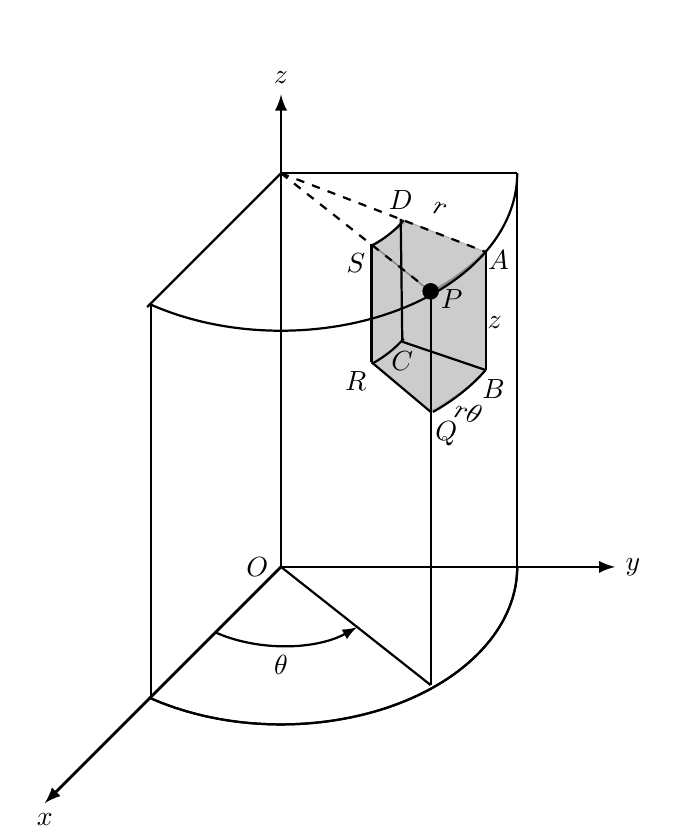
\begin{tikzpicture}[scale=1]
        \coordinate (O) at (0,0);
        \coordinate (Ox) at (-3,-3);
        \coordinate (Oy) at (4.243,0);  % sqrt{18}
        \coordinate (Oz) at (0, 6);

        % draw axis
        \draw[-latex, line width=1] (O)-- (Ox) node[below] {$x$};
        \draw[-latex, line width=1] (O)-- (Oy) node[right] {$y$};
        \draw[-latex, line width=1] (O)-- (Oz) node[above] {$z$};


        % draw arcs
        \draw[thick] ($(0, 0) + (236:3cm and 2cm)$(P) arc
        (236:360:3cm and 2cm);
        \draw[thick] ($(0, 0) + (236:3cm and 2cm)$(P) arc
        (236:360:3cm and 2cm);

        \draw[thick] ($(0, 5) + (236:3cm and 2cm)$(P) arc
        (236:360:3cm and 2cm);

        \draw[thick, -latex] ($(0, 0) + (236:1.5cm and 1cm)$(P) arc
        (236:310:1.5cm and 1cm);

        \coordinate (Phi) at (0,-1) ;
        \node[below] at (Phi) {$\theta$};


        \coordinate (A1) at (0, 5);
        \coordinate (B) at (3, 5);
        \coordinate (C) at (-1.7, 3.3);
        \draw[thick] (A1)--(B);
        \draw[thick] (A1)--(C);



        % radius
        \coordinate (D) at (1.9,-1.5);
        \coordinate (P) at (1.9,3.5);
        \draw[thick] (O)--(D);
        \draw[thick, dashed] (A1)--(P) node[right, yshift=-1mm] {$P$};
        \draw[thick] (D)--(P);
        \fill[black] (P) circle (3pt);


        \coordinate (A) at (2.6, 4.0);
        \draw[thick, dashed] (A1)--(A) node[right, yshift=-1mm, xshift=-1mm] {$A$};


        % arcs
        \draw[thick] ($(0, 5) + (310:1.8cm and 1.2cm)$(P) arc
        (310:330:1.8cm and 1.2cm);

        \draw[thick] ($(0, 3.5) + (310:1.8cm and 1.2cm)$(P) arc
        (310:330:1.8cm and 1.2cm);

        \draw[thick] ($(0, 3.5) + (310:3cm and 2cm)$(P) arc
        (310:330:3cm and 2cm);

        \coordinate (Q) at (1.9,1.97);
        \node[below,xshift=2mm] at (Q) {$Q$};
        \node[xshift=-3mm] at (O){$O$};
        % \fill[black] (Q) circle (3pt);


        \coordinate (B) at (2.6, 2.5);
        \node[below,xshift=1mm] at (B) {$B$};
        % \fill[black] (B) circle (3pt);
        \draw[thick] (A) --(B);

        \coordinate (S) at (1.15, 4.1);
        \node[below, xshift=-2mm] at (S) {$S$};
        % \fill[black] (S) circle (3pt);

        \coordinate (R) at (1.15, 2.6);
        \node[below, xshift=-2mm] at (R) {$R$};
        %\fill[black] (R) circle (3pt);


        \coordinate (D) at (1.52, 4.42);
        \node[above] at (D) {$D$};
        % \fill[black] (D) circle (3pt);

        \coordinate (C) at (1.54, 2.86);
        \node[below] at (C) {$C$};
        %\fill[black] (C) circle (3pt);

        \draw[thick] (S) --(R);
        \draw[thick] (D) --(C);
        \draw[thick] (R) --(Q);
        \draw[thick] (C) --(B);

        % verticals on the planes
        \coordinate (H) at (-1.65,-1.65);
        %\fill[black] (H) circle (3pt);
        %
        \coordinate (I) at (-1.65,3.35);
        %\fill[black] (I) circle (3pt);
        \draw[thick] (H) --(I);

        \coordinate (J) at (3,0);
        %\fill[black] (J) circle (3pt);
        \coordinate (K) at (3,5);
        %\fill[black] (K) circle (3pt);
        \draw[thick] (J) --(K);

        % filling
        \filldraw[opacity=0.2]
        (D)--(A) arc (325:306:3cm and 2.2cm)--(S)
        arc (305:325:1.8cm and 1.2cm)--cycle;

        \filldraw[opacity=0.2]
        (P) arc (306:325:3cm and 2.2cm)--(B)
        arc (325:306:3.0cm and 2.2cm)--cycle;

        \filldraw[opacity=0.2]
        (P)--(Q)--(R)--(S)--cycle;

        % differential labels
        \node[right, yshift=1mm,xshift=2mm, rotate=-20] at (Q) {$r \dif \theta$};
        \node[right, yshift=6mm, xshift=-1mm ] at (B) {$\dif z$};
        \node[right,xshift=3mm, yshift=2mm, rotate=-20] at (D) {$\dif r$};

    \end{tikzpicture}
    \refstepcounter{figure}

    图\thefigure: 柱坐标系\footnote{本图来自 \url{https://www.latexstudio.net/index/details/index/mid/813.html}}
\end{minipage}
\begin{minipage}{0.35\textwidth}
    如图,这是一个以$x$轴为极轴的柱坐标系,$P$的坐标为$(r,\theta,z)$。
    \[\vec{OP}=\vec{r}+\vec{z}\]
    阴影部分是一个极小的体积元(这里放大绘制)。
\end{minipage}
\vspace{2ex}

在对刚体运动进行描述时,我们往往选取刚体的旋转轴作为$z$轴建立柱坐标系,然后借助柱坐标系说明其运动的相关参数。


\subsection[叉乘]{\itr{Cross Product}{叉乘}\labelroot[16pt]{chapter3_cross_product}}
在介绍转动的有关概念前,我们还需引入叉乘这一数学工具。

由于叉乘的具体内容介绍属于线性代数与数学分析的任务,这里并不会展开讲。

叉乘可以看成这样一个运算:按顺序输入两个向量$\vec{A},\vec{B}$,输出一个特定长度且与它们都正交的向量$\vec{C}$。当然,这样的描述是不精确的,一是长度需要确定的值,二是与$\vec{A},\vec{B}$都正交的向量方向不唯一\mgnote{除了$\vec{0}$,还有正反两个方向}。因此,接下来,我们要对长度和方向作出具体描述。

\begin{Itemize}
    \item 长度: $C=AB\sin\theta$,其中$\theta$是由$\vec{A}$旋转至$\vec{B}$所成的小于$\dfrac{\pi}{2}$的角\footnotemark 。在几何意义上,$|\vec{C}|$即是$\vec{A},\vec{B}$构成的平行四边形的面积。
    \item 方向: $\vec{C}$的方向是介绍长度时所述的$\vec{\theta}$的方向\mgnote{关于角度矢量的方向,可回见\\\refleaftext{chapter3_direction}。}。在几何意义上,$\vec{C}$与$\vec{A},\vec{B}$所张成平面的法向量平行。
\end{Itemize}
\footnotetext{事实上,这里不规定旋转,对于长度是没有影响的。这里这么说,主要是希望在介绍长度和方向时,这个角度可以统一。回想一下,在介绍极坐标系时,我们就规定逆时针是正方向了,所以这么规定可以合理地引出正负。}

如果这么说不够直观,我们可以参考右手定则:

\begin{singlefigure}[\En{Right-Hand Rule}]{chapter3_right_hand_rule}[0.6]
    以$\vec{A}$为起始,右手手指向$\vec{B}$弯曲(取$<\frac{\pi}{2}$方向),大拇指方向为$\vec{C}$的方向\\
    我们称$\vec{A}$叉乘$\vec{B}$等于$\vec{C}$,记作$\vec{A}\times\vec{B}=\vec{C}$
\end{singlefigure}

下面不加证明地给出叉乘的有关性质和定理:

\begin{Itemize}
    \item \itr{Anti-Commutative Law}{反交换律} $\vec{A}\times\vec{B}=-\vec{B}\times\vec{A}$,即交换两向量顺序,它们的夹角方向会取反。
    \item \itr{Distributive Law}{分配律} $\vec{A}\times(\vec{B}+\vec{C})=\vec{A}\times\vec{B}+\vec{A}\times\vec{C}$
    \item \itr{Derivative}{导数} $\dfrac{\dif}{\dif t}(\vec{A}\times\vec{B})=\dfrac{\dif\vec{A}}{\dif t}\times \vec{B}+\vec{A}\times\dfrac{\dif\vec{B}}{\dif t}$\labelroot{chapter3_derivation}\\
    \En{It is important to preserve the
        multiplicative order of A and B.}\\
    鉴于反交换率,保证叉乘的顺序正确是十分重要的。
    \item \itr{Lagrange's Identity}{拉格朗日恒等式} $(\vec{A}\times\vec{B})\cdot(\vec{C}\times\vec{D})=\left|\begin{array}{cc}
            \vec{A}\cdot\vec{C} & \vec{A}\cdot\vec{D} \\
            \vec{B}\cdot\vec{C} & \vec{B}\cdot\vec{D}
        \end{array}\right|$
    \item \itr{Double Cross Product}{二重叉乘}\labelroot{chapter3_double_cross_product}\begin{align*}
        (\vec{A}\times\vec{B})\times\vec{C} & =(\vec{A}\cdot\vec{C})\vec{B}-(\vec{B}\cdot\vec{C})\vec{A} \\
        \vec{A}\times(\vec{B}\times\vec{C}) & =(\vec{A}\cdot\vec{C})\vec{B}-(\vec{A}\cdot\vec{B})\vec{C}
    \end{align*}
    这里也可以发现,叉乘不满足结合律。
\end{Itemize}

有些同学初次看见那么多公式难免慌张。事实上,普通物理\Romannumeral{1}对于叉乘的考察非常有限,基本只要清楚定义和基本的运算律即可。
\subsection[运动学概念]{\itr{Concepts in Kinematics}{运动学概念}}
%\textit{为了保证分析的简单,除非特别说明,我们默认,选择的旋转轴方向总是与角速度方向平行}。

在定好一个柱坐标系后之后,确定刚体的角度矢量及其与时间的关系,就能确定刚体的转动。

\begin{Itemize}
    \item \itr{Angular displacement}{角位移}\mgnote{$\vec{\theta}$的单位rad属于数学单位,它是一个无量纲量。} $\Delta\vec{\theta}=\vec{\theta}_f-\vec{\theta}_i$
    \item \itr{Instantaneous angular velocity}{瞬时角速度} $\vec{\omega} = \dfrac{\dif\vec{\theta}}{\dif t}$
    \item \itr{Instantaneous angular acceleration}{瞬时角加速度}  $\vec{\alpha}=\dfrac{\dif\vec{\omega}}{\dif t}$
\end{Itemize}

\En{When rotating about
    a fixed axis, every
    particle on a rigid
    object rotates
    through the same
    angle and has the
    same angular speed
    and the same angular
    acceleration.}

平动与转动有如下关系\labelroot{chapter3_connection}:
\begin{Itemize}
    \item  \itr{arc length}{弧长} $s=r\theta$,此指圆周运动。
    \item $\vec{v}_t=\vec{\omega}\times\vec{r}$ \& $v_t=\omega r$,其中t下标指\itr{tangential}{切向},$\vec{v}_t$即同时垂直于$z$轴\footnotemark 和$\vec{r}$的速度分量。
    \item $\vec{a}_t=\vec{\alpha}\times\vec{r}$ \& $a_t=\alpha r$,$\vec{a}_t$即同时垂直于$z$轴和$\vec{r}$的加速度分量。
\end{Itemize}
\footnotetext{注意这里垂直于$z$轴的条件,我们考虑的是绕轴旋转,所以任何轴向的速度分量也不在我们研究转动的考虑之中。}

这里叉乘的先后顺序可能并不那么好记,推荐读者自己画一个圆周运动的图,用右手定则对应验证一遍如上关系,以加深理解与记忆。

\subsection[动力学概念]{\itr{Concepts in Dynamics}{动力学概念}}
在引入了叉乘(见\refleaftext{chapter3_cross_product})这一数学工具后,我们得以较为轻松地描述转动的动力学概念。

以下默认已经选定转轴\labelroot{chapter3_axis}。

\begin{Itemize}
    \item \itr{The Moment of Inertia}{转动惯量} $\displaystyle I=\sum_{i}m_ir_i^2$,其中把刚体看成由多个质点组合而成,$r_i$即是质点$m_i$的极径矢量大小。

    \En{The moment of inertia is a measure of the
        resistance of an object to changes in its rotational
        motion, just as mass is a measure of the tendency
        of an object to resist changes in its linear motion.}
    \item \itr{Torque}{力矩} $\vec{\tau}=\vec{r}\times\vec{F}_{/z}$,其中$\vec{r}$是力$\vec{F}$的作用点对应的极径矢量,$\vec{F}_{/z}=\vec{F}-\vec{F}_z$,$\vec{F}_z$即$\vec{F}$在$z$轴上的分矢量\labelroot{chapter3_lower/z}\footnotemark。
    \item \itr{Net Torque}{合外力矩} $\displaystyle\vec{\tau}_{net}=\sum_{i}\vec{\tau}_i$
    \item 类似牛顿第二定律,有:在惯性系中,$\vec{\tau}_{net}=I\vec{\alpha}$,即合外力矩等于刚体的转动惯量乘以角加速度。
\end{Itemize}
\footnotetext{事实上,力矩拥有两种定义,一种是对点定义的,为$\vec{r}\times\vec{F}$;另一种是对轴定义的,为$\vec{r}\times\vec{F}_{/z}$。鉴于我们使用了柱坐标系建立这些概念,这里选择对轴定义的力矩。}
\begin{singlefigure}[力矩示意图]{chapter3_torque}[0.5]
    在本图中,由于$\vec{F}$没有$z$轴上的分量,所以$\vec{F}=\vec{F}_{/z}$。\\
    事实上,普物\Romannumeral{1}中基本没有出现过$\vec{F}$有$z$轴分量的情况。
\end{singlefigure}
关于以上内容的证明,见\refleaftext{prove3.1}。

其中,为了便于计算力矩,我们可以引入 \itr{moment arm/force arm}{力臂} 的概念,其大小即为转轴到力的作用线的距离。有了这一点,力矩的大小就可以通过力臂乘以力得到。
\ctikzfig{chapter3_moment_arm}
\begin{center}
    \em $l_1$是$\vec{F}_1$的力臂,$l_2$是$\vec{F}_2$的力臂。
\end{center}

对于常见的物体,其转动惯量是应当记住的:
\begin{singlefigure}{chapter3_moment_inertia1}
\end{singlefigure}
\vspace*{-2ex}
\begin{singlefigure}[常见物体的转动惯量]{chapter3_moment_inertia2}
\end{singlefigure}
对于更一般的物体,则往往通过积分的方式求取它们的转动惯量。
\section[平行轴定理/施泰纳定理]{\itr{Parallel Axis Theorem/Steiner Theorem}{平行轴定理/施泰纳定理}}
在之前对转动的动力学概念的讨论中,我们默认转轴是选定的\mgnote{见\refleaftext{chapter3_axis}},这是因为,当转轴不同时,转动惯量与合力矩都会发生变化。平行轴定理是解决转轴变化过程中转动惯量变化的利器,其表述如下:

\begin{law}[\itr{Parallel Axis Theorem/Steiner Theorem}{平行轴定理/施泰纳定理}---\refleaftext{prove3.2}]
    记刚体$M$以过质心的轴(简称质心轴)为转动轴时的转动惯量为$I_{CM}$,以任意平行于质心轴的轴为转动轴时的转动惯量为$I$,这两条轴之间的距离为$h$,则有
    \[I=I_{CM}+Mh^2\]
\end{law}

幸于拥有平行轴公式,我们在背诵常见刚体的转动惯量时,一般只要记下它以质心轴为转动轴时的转动惯量即可。

\section[刚体中的能量]{\itr{Energy in a Rigid Body}{刚体中的能量}}
好比从牛顿三律进发到能量定律,我们将开始研究刚体中的能量。
\subsection[纯转动中的能量]{\itr{Energy in Rotation ONLY}{纯转动中的能量}}
首先,让我们思考一个只发生转动的刚体所带的能量(\refleaftext{prove3.3})。
\begin{Itemize}
    \item 动能定理 $K_R=\dfrac{1}{2}I\omega^2$
    \item 做功 $\dif W=\tau\dif\theta$
    \item 功率 $P=\tau\omega$
    \item 旋转势能 $U=\dfrac{1}{2}\kappa\theta^2$
\end{Itemize}
其中,旋转势能是指由弹性旋转体扭转回原位的趋势产生的,只依赖于其状态的能量,在数值上等于将旋
转体自原位扭转至当前位置所做的功。$\kappa$称为扭转常数,单位为$\mathrm{N}\cdot\mathrm{m}$。

当旋转体扭转了角度$\vec{\theta}$时,就会产生反力矩$\vec{\tau}=-\kappa\vec{\theta}$。
\subsection[同时发生转动与平动时的能量]{\itr{Energy in Rotation \& Translation}{同时发生转动与平动时的能量}}
现在,让我们思考一个问题:
\begin{center}
    \itshape 一个刚体在质心系中能够发生平动吗?
\end{center}

答案是否定的。如果刚体在质心系中发生平动,那么质心就会拥有平动速度,然而,在质心系中,质心又一直处于原点,这与质心拥有平动速度相矛盾,因此刚体在质心系中只能发生转动\labelroot{chapter3_rotation_CM}。

既然如此,我们便会有这样的想法:利用质心系,把同时发生平动和转动的物体转化成只发生转动的物体来研究。如此,便产生了柯尼希定理:

\begin{law}[\itr{Konig's Theorem}{柯尼希定理}---\refleaftext{prove3.4}]
    记一个系统$M$的质心速度为$v_{_{CM}}$,在质心系中的动能为$K^{CM}$,在静止参考系中的动能为$K$,并记$K_{CM}=\dfrac{1}{2}Mv_{_{CM}}{}^2$,则有
    \[K=K_{CM}+K^{CM}\]
    如果考虑对一个刚体使用柯尼希定理,则有:
    \[K=\dfrac{1}{2}Mv_{_{CM}}{}^2+\dfrac{1}{2}I_{CM}\omega^2\]
\end{law}

在研究一个同时发生平动和转动的物体的动能时,我们往往使用柯尼希定理,分别求解其质心的平动动能和在质心系中的转动动能。
\section[角动量]{\itr{Angular Momentum}{角动量}}
与平动时的动量类似,我们可以定义刚体的角动量。
\subsection[定义]{Definition}
\begin{Itemize}
    \item \itr{Angular Momentum}{角动量} $\displaystyle\vec{L}=\sum_i\vec{r}_i\times\vec{p}_{i/z}=I\vec{\omega}$,其中$\vec{p}_{i/z}=\vec{p}_i-\vec{p}_{iz}$,$ \vec{r}_i\times\vec{p}_{i/z}$应视作质点$m_i$的角动量。角动量的方向总是与角速度的方向一致\footnotemark。
    \item 类似动量,我们有$\dfrac{\dif \vec{L}}{\dif t}=\vec{\tau}_{net}$。
\end{Itemize}
以上内容证明见\refleaftext{prove3.5}。

\footnotetext{对于这句话需持谨慎态度。在本章所定义的概念体系中,这句话是成立的,但由于大多数对角动量的定义都是对点定义,即$\displaystyle\sum_i\vec{r}_i\times\vec{p}_i$,就出现了角动量方向与角速度方向不一致的说法。\textbf{当出现这类判断时,请读者优先考虑不一致的说法}。}
\subsection[角动量守恒]{\itr{Conservation of Angular Momentum}{角动量守恒}}
\begin{Itemize}
    \item \itr{Conservation of Angular Momentum}{角动量守恒}由角动量的性质,我们可以发现,当合外力矩的值为$\vec{0}$时,系统的角动量保持守恒。
    \[\vec{\tau}_{net}=0\Leftrightarrow\vec{L}=Constant\]
\end{Itemize}

利用角动量守恒,可以解释开普勒第二定律。
\begin{singlefigure}[\En{Kepler's Second Law}]{chapter3_kepler's_second_law}
    对$M_p$分析,有$\vec{\tau}_{net}=\vec{r}\times\vec{F}_g=\vec{0}$,因此角动量守恒\\[1ex]
    $\dfrac{\dif A}{\dif t}=\dfrac{1}{2}|\vec{r}\times\vec{v}|=\dfrac{L}{M_p}\Rightarrow$单位时间扫过面积相等
\end{singlefigure}
\En{When a force is directed toward or away from a
    fixed point and is function of $\vec{r}$ only, it is called a
    \itr{Central Force}{中心力}.}

总是可以选择合适的轴,使得中心力产生的力矩为$\vec{0}$。

花样滑冰时选手收紧胳膊旋转较快,而张开双臂后旋转变
慢,这也是角动量守恒的功劳。你可能会发现,收紧胳膊时,人的动能变大了,这是生物能的功劳。
\subsection[质心系转化]{\itr{Center of Frame Translation}{质心系转化}}
角动量在静止参考系和质心系间的转化与柯尼希定理类似。
\begin{law}[\itr{Angular Momentum Translation Using C.M. Frame}{利用质心系的角动量变换}\footnotemark---\refleaftext{prove3.6}]
    记质心角动量为$\vec{L}_{CM}=M\vec{r}_{_{CM}}\times\vec{v}_{_{CM}}$,刚体在质心系中的角动量为$\vec{L}^{CM}=\sum_im_i\vec{r}_i^{^{CM}}\times\vec{v}^{^{CM}}_i$,刚体在静止参考系中的角动量为$\vec{L}$,且保证两个参考系中选取的轴平行,则有
    \[\vec{L}=\vec{L}_{CM}+\vec{L}^{CM}\]
\end{law}
\footnotetext{对于对点定义的角动量,也有类似的结论,证明方法也基本相同。}
\section[重心]{\itr{Center of Gravity}{重心}}
我们会注意到,在分析重力产生的合力矩时,依据定义,应该对每一个质元求分力矩,然后进行求和。这似乎是一件复杂的事情。有没有办法寻找一个点,使得刚体的合重力在此作用时,得到的力矩恰等于重力的合力矩呢?事实上,我们把这样的点称作重心。

一个重要的结论是:
\begin{center}
    {\itshape 对于均匀的重力场,刚体的重心与质心重合(\refleaftext{prove3.7})}。
\end{center}

至于不均匀的情况,就需要依据定义进行计算了。
\section[非惯性系情形]{\itr{Non-Inertial Frame Situation}{非惯性系情形}}
\subsection[非惯性力]{\itr{Inertial Force}{惯性力}}
由于转动动力学的所有定律都是基于牛顿运动定律,结合数学方法推出的,因此,对于一个拥有加速度$\vec{a}_{frame}$的平动非惯性参考系\labelroot{chapter3_translation},我们需要在分析其中的物体时添上惯性力$\vec{F}_{fictious}=-m\vec{a}_{frame}$,其中$m$为物体的质量。此时,牛顿运动定律保持成立,转动动力学中的定律也保持成立。

\subsection[科里奥利力*]{\itr{Coriolis Force}{科里奥利力}*}
你可能注意到了,之前的表述中,我们讲的是“拥有加速度$\vec{a}_{frame}$的平动非惯性参考系”\mgnote{见\refleaftext{chapter3_translation}}。这暗示着,如果参考系还发生着转动,情况又会有所不同。

对于一个仅发生转动的参考系,有如下定理:
\begin{law}[\itr{Frame Translation with Rotation}{考虑转动的参考系变换}$^*$---\refleaftext{prove3.8}]
    如果希望牛顿运动定律在一个转动参考系$\mathcal{F}'$中依然成立,我们需要对$\mathcal{F}'$中的物体添加三个假想力,分别是$-2m\vec{\omega}\times\vec{v}',-m\vec{\alpha}\times\vec{r}',m\omega^2\vec{r}'$。

    其中,$\vec{\omega}$是$\mathcal{F}'$的角速度,$\vec{\alpha}$是$\mathcal{F}'$的角加速度,$\vec{v}'$是物体在$\mathcal{F}'$中的速度,$\vec{r}'$是物体在$\mathcal{F}'$中的极径矢量。

    如果我们将条件简化,认为$\mathcal{F}'$没有角加速度,则无需考虑$-m\vec{\alpha}\times\vec{r}'$。

    我们称$-2m\vec{\omega}\times\vec{v}'$为 \itr{Coriolis Force}{科里奥利力},$m\omega^2\vec{r}'$为 \itr{Centrifugal Force}{离心力}。
\end{law}
\begin{singlefigure}[地球的科里奥利力]{chapter3_earth}[0.42]
    如果考虑地球的科里奥利力,我们会发现,在北半球上,\\科里奥利
    力永远指向物体运动方向的右侧,而在南半球正好相反。
\end{singlefigure}
台风的旋转方向在北半球是逆时针,在南半球是顺时针,这也是科里奥利力的影响。

{\bfseries 科里奥利力是一种假想力}\footnote{我们有时会看见类似“科里奥利力是由于地球自转而施加给地球上的物体的力”的说法,这么讲可能是因为我们往往以地球为参考系分析问题,此时要想保证牛顿第二定律成立,就要认为物体受到科里奥利力。不过,一般而言,科里奥利力较小,在日常生活的分析中大多可忽略不计。}。
\section[回顾与总结]{Review and Summary}
在我们的推导中,我们发现,转动力学的结论与平动力学有着惊人的相似性。关注这份相似性既能体会物理的美感,又能加深对结论的记忆。
\[\ \ \begin{aligned}
         & \mathrm{Angular~speed~}\vec{\omega}=\dif\vec{\theta}/\dif t                                                                                                          &   & \mathrm{Linear~speed~}\vec{v}=\dif \vec{x}/\dif t         \\
         & \mathrm{Angular~acceleration~}\vec{\alpha}=\dif\vec{\omega}/\dif t                                                                                                   &   & \mathrm{Linear~acceleration~}\vec{a}=\dif \vec{v}/\dif t  \\
         & \mathrm{Resultant~torque~}\sum\vec{\tau}=I\vec{\alpha}                                                                                                               &   & \mathrm{Resultant~force~}\sum \vec{F}=m\vec{a}            \\
         & \begin{array}{l}{{\mathrm{If}}}\\{\vec{\alpha}=\mathrm{constant}}\left\{\begin{array}{l}{{\vec{\omega}_{f}=\vec{\omega}_{i}+\vec{\alpha} t}}\\{{\vec{\theta}_{f}-\vec{\theta}_{i}=\vec{\omega}_{i}t+\frac{1}{2}\vec{\alpha} t^{2}}}\\{{\omega_{f}{}^{2}=\omega_{i}{}^{2}+2\alpha(\theta_{f}-\theta_{i})}}\end{array}\right.\end{array}
         &                                                                                                                                                                      &
        \begin{array}{l}{{\mathrm{If}}}\\{\vec{a}=\mathrm{constant}}\left\{\begin{array}{l}{{\vec{v}_{f}=\vec{v}_{i}+\vec{a}t}}\\{{\vec{x}_{f}-\vec{x}_{i}=\vec{v}_{i}t+\frac{1}{2}\vec{a}t^{2}}}\\{{v_{f}{}^{2}=v_{i}{}^{2}+2a(x_{f}-x_{i})}}\end{array}\right.\end{array}                                                                         \\
         & \mathrm{Work}\ W=\int_{\theta_{i}}^{\theta_{f}}\tau \dif\theta                                                                                                       &   & \mathrm{Work}\ W=\int_{x_{i}}^{x_{f}}F_{x}\dif x          \\
         & \mathrm{Rotational~kinetic~energy~}K_{\mathrm{R}}=\frac{1}{2}I\omega^{2}                                                                                             &   & \mathrm{Kinetic~energy~}K=\frac{1}{2}mv^{2}               \\
         & \mathrm{Power}\ P=\vec{\tau}\cdot\vec{\omega}                                                                                                                        &   & \mathrm{Power}\ P=\vec{F}\cdot\vec{v}                     \\
         & \mathrm{Angular~momentum~}\vec{L}=I\vec{\omega}                                                                                                                      &   & \mathrm{Linear~momentum~}\vec{p}=m\vec{v}                 \\
         & \mathrm{Resultant~torque~}\sum\vec{\tau}=\dif \vec{L}/\dif t                                                                                                         &   & \mathrm{Resultant~force~}\sum \vec{F}=\dif \vec{p}/\dif t
    \end{aligned}\]












\newpage
\section{课后习题:转动动力学}
\begin{example}[{\small Determine the Moment of Inertia of an Irregularly Shaped Object}---\refleaftext{solution3.1}]
	This problem describes one experimental method of
	determining the moment of inertia of an irregularly
	shaped object such as the \itr{payload}{有效负载} for a satellite. 
	\begin{center}
		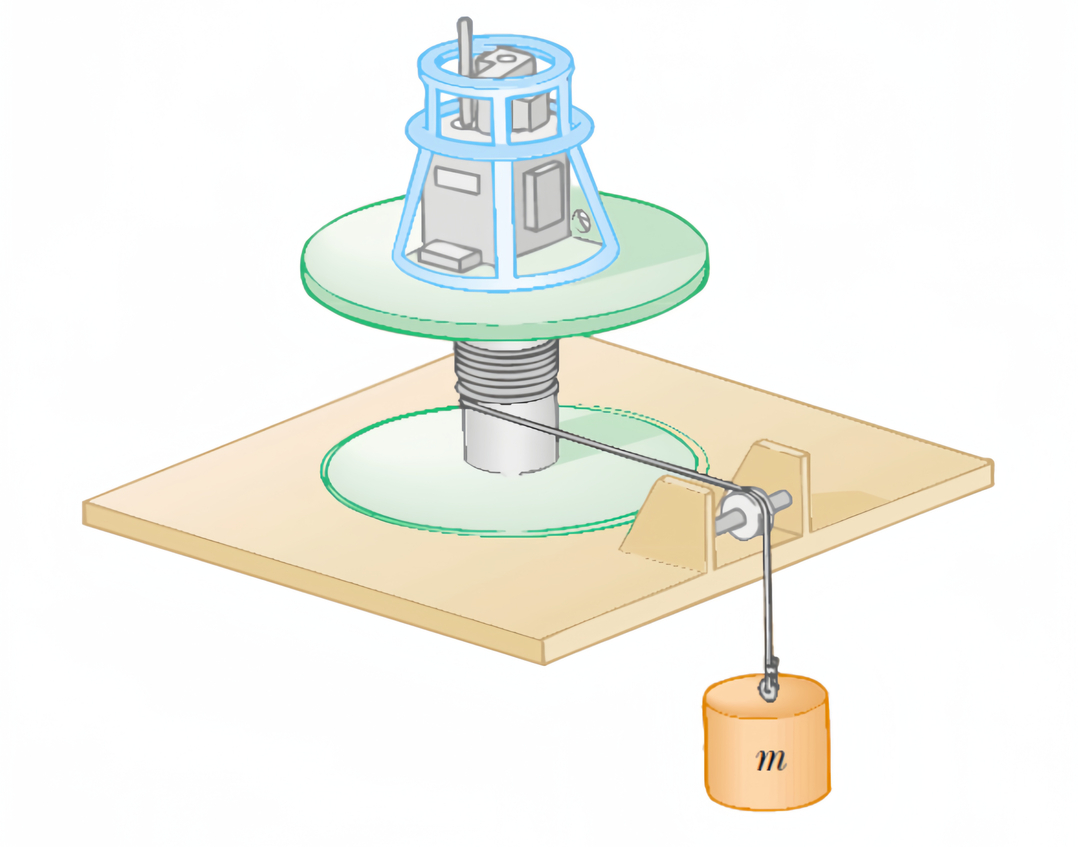
\includegraphics[width=0.6\textwidth]{chapter3_example_1}
	\end{center}
	
	The figure shows a mass $m$ \itr{suspended}{悬挂} by a \itr{cord}{绳子} \itr{wound}{被缠绕}
	around a spool of radius $r$, forming part of a \itr{turntable}{转台}
	supporting the object. When the mass is released from
	rest, it \itr{descends}{下降} through a distance $h$, acquiring a speed
	$\vec{v}$. Show that the moment of inertia $I$ of the equipment
	(including the turntable) is\quad$mr^2(\dfrac{2gh}{v^2}-1)$. 
\end{example}
%\refleaf*{solution3.1}[-75ex]
\begin{example}[Rolling Items---\refleaftext{solution3.2}]
	Three objects of \itr{uniform density}{均匀的密度} --- a \itr{solid sphere}{实心球}, a \itr{solid
	cylinder}{实心圆柱}, and a \itr{hollow cylinder}{空心圆柱} --- are placed at the top of
	an \itr{incline}{斜坡}. 
	\begin{center}
		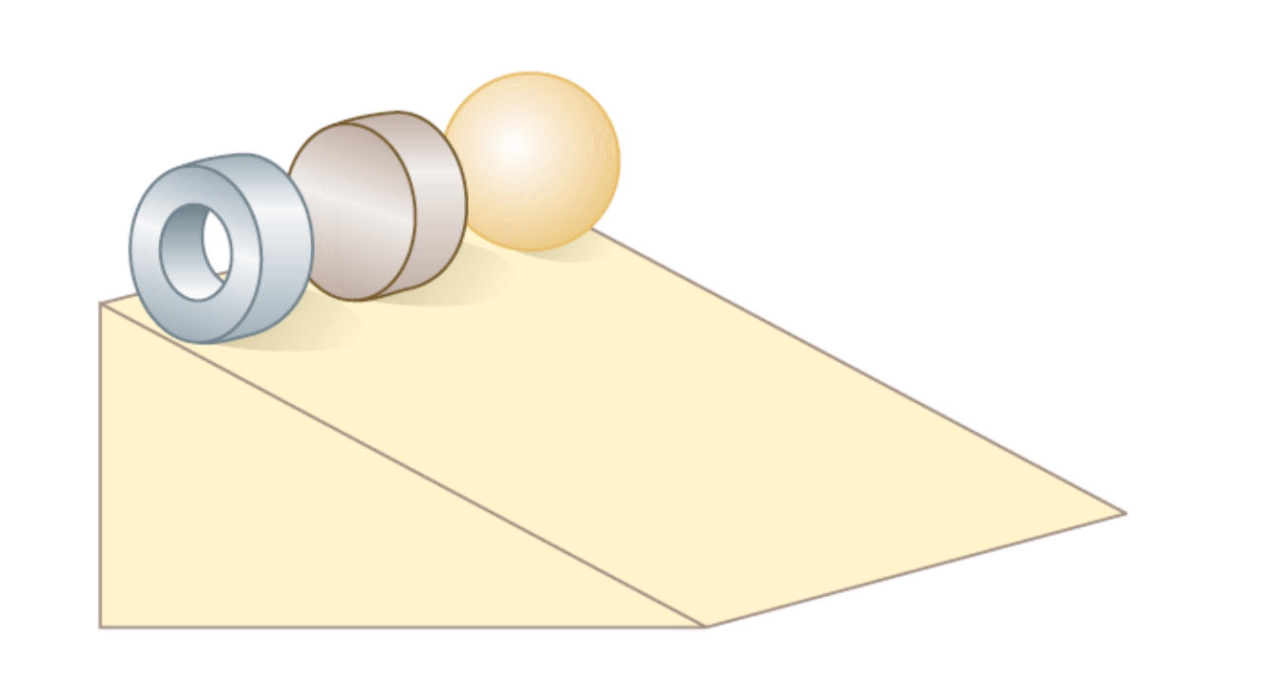
\includegraphics[width=0.6\textwidth]{chapter3_example_2}
	\end{center}
	If they all are released from rest
	at the same \itr{elevation}{高度} and roll without \itr{slipping}{滑动}, which object reaches the bottom first?
\end{example}
%\refleaf*{solution3.2}[-20ex]
\begin{example}[Calculation of the Moment of Inertia---\refleaftext{solution3.3}]
	A rod's \itr{linear density}{线密度} is given by $\lambda=kx$, where $x$ represents the distance from the point to the rod's center. 
	\begin{singlefigure}{chapter3_rod}[0.5]
	\end{singlefigure}
	Given the length of the rod $l$, try to calculate the moment of inertia of the rod, given the rotation axis at:
	
	(1) Center $O$ as the $y$ axis shows.
	
	(2) One end as the $y'$ axis shows.
\end{example}
\begin{example}[Massive \itr{Pulley}{滑轮}---\refleaftext{solution3.4}]
	Consider two \itr{cylinders}{圆柱} having masses $m_1$
	and $m_2$, where $m_1 < m_2$, connected by a
	string passing over a pulley. The pulley
	has a radius $R$ and moment of inertia $I$
	about its axis of rotation.
	\begin{singlefigure}{chapter3_massive_pulley}[0.3]
		The string does
		not \itr{slip}{滑动} on the pulley, and the system
		is released from rest. 
	\end{singlefigure}
	 Find the linear
	speeds of the cylinders after
	cylinder 2 \itr{descends}{下降} through a
	distance $h$, and the angular
	speed $\omega$ of the pulley at this time.
\end{example}
\begin{example}[Object rotating on a string
	of changing length---\refleaftext{solution3.5}]
	Initially, the mass \itr{revolves}{转动} with a speed $v_1$ = 2.4 m/s in
	a circle of radius $R_1$ = 0.80 m.
	The string is then pulled slowly through the hole so
	that the radius is reduced to $R_2$ = 0.48 m. What is the
	speed, $v_2$, of the mass now?
	\begin{singlefigure}{chapter3_string}[0.7]
	\end{singlefigure}
\end{example}
\begin{example}[Rotation of a sliding rigid rod---\refleaftext{solution3.6}]
	Consider a rod with mass m and length L standing straight on the friction-less ground. When we
	release the rod, it will fall from the unstable \itr{equilibrium position}{平衡位置}.
	\begin{center}
		\begin{minipage}{0.45\textwidth}
			\centering
			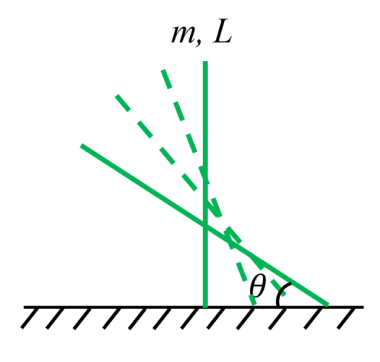
\includegraphics[width=\linewidth]{chapter3_rotating_rod_1}\\
			Figure 1
		\end{minipage}
		\quad
		\begin{minipage}{0.45\textwidth}
			\centering
			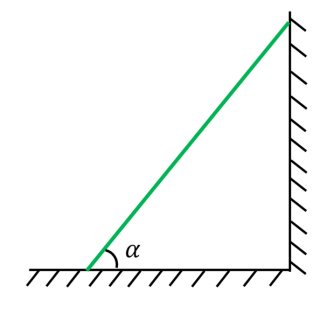
\includegraphics[width=\linewidth]{chapter3_rotating_rod_2}\\
			Figure 2
		\end{minipage}
	\end{center}
	(a) Calculate the angular velocity of the rod, when it has an angle of $\theta$ with respect to the ground
	as illustrated in Figure 1.\\
	(b) What is the final angular velocity $\omega_1$ of the rod before it hits the ground?\\
	(c) If the same rod is leaning to a frictionless wall with an initial angle of α to the frictionless
	ground (see Figure 2), what is the final angular velocity $\omega_2$ of the rod before it hits the ground?\\
	{\em Note that there is a possibility that the right end of the rod leaves from the wall before the rod hits the ground.}
\end{example}
\begin{comment}
    \documentclass{Physics_H_Notes}
    \usepackage{upgreek}
    \begin{document}
    \end{comment}
        \chapter[流体力学]{\itr{Fluid Mechanics}{流体力学}\mgnote*{\raggedleft 作者:22级-薛宇航}}
        本章节存在一定的特殊性:在2022年及之前,流体力学是普物\Romannumeral{1}的内容,而在2023级,这一块内容被路欣老师为代表的教学组删去了。

        当看到流体力学的时候,你想到的是什么?或许是初中的水的压强,又或者是湍流等复杂情景。其实都无所谓,毕竟它们都是流体的研究。当今世界对于流体力学的探究也是一个重要的力学方向,小到潜水,大到飞机飞船,都需要关注流体对于物体的影响。
        但是,我们这门课程的流体力学相当简单和浅层,按照笔者当时授课较为简单的pzq老师的内容,我用一句话定义这一块内容:两个公式走天下!这是由于我们使用了大量的理想情景,抛除复杂情景所致。
        \section[流体的定义与性质]{\itr{Definition \& Properties of Fluids}{流体的定义与性质}}
        生活中的物体可分为固体、液体和气体三大类,其中,我们一般将液体和气体统称为流体。它们一般受到的力是不一样的:
        \begin{Itemize}
            \item \itr{solid}{固体}: \itr{compression force}{压缩力}(指物体能够从两侧被挤压), \itr{tensile force}{拉力}(指物体能够受力被拉伸), 
                \itr{shearing force}{剪切力}(指物体能够受到不在同一直线上的两个相反方向的力而保持形状不变)
            \item \itr{liquid}{液体}: compression force, tensile force, no shearing force
            \item \itr{gas}{气体}: compression force, no tensile force, no shearing force
        \end{Itemize}
        
        在静止的液体中,我们已经了解到物体一定会受到水的压力,进而定义压强。
        \begin{law}[静止流体中的压强]
            利用微元法分析,我们可以知道物体受到的静止流体的压强为:
            \begin{center}
                $\dfrac{\dif p}{\dif y}=-\rho g$,积分可得$p=p_0+\rho gh$
            \end{center}

            其中$p_0$是液体表面的压力,$h$为深度,$y$为该点相对于参考平面的高度。
        \end{law}
        
        对于静止流体,我们也有两个重要的而且很直观的性质:
        \begin{law}[\itr{Pascal's Principle}{帕斯卡原理}]
            施加在封闭流体上的力被不减弱地传递到流体的每一部分和容器的壁上。假设流体中受力面积为$S$的某点处原有压强为$p_0$,在其上方平面施加垂直向下的力$F$,则该点处当前的压力为:
            \begin{center}
                $F^{'}=p_0 S +F$
            \end{center}
        \end{law}

        这是很容易理解的,我们以按压海绵为例,力的作用会逐渐传导到物体的每个位置。当然,帕斯卡原理强调了在流体中这个力是不会减弱的,
        而海绵是固体,力是会减弱的。
        \begin{law}[\itr{Archimedes's Principle}{阿基米德原理}]
            一个部分或者完全浸入液体中的物体受到的浮力等同于它所排出的液体的重力。
        \end{law}

        最简单的例子,就是我们初中学过的物体受到水的浮力的公式:
        \begin{center}
            $F=\rho gV$
        \end{center}

        我们可以很容易地知道这个公式的本质就是阿基米德原理。

        在液体中存在表面张力,表面张力是一种由于液体分子间的相互吸引与拉扯而产生的力的作用,其大小与物体间的接触长度有关。定义表面张力系数为:
        \begin{center}
            $\gamma =\dfrac{F}{l}$
        \end{center}

        其中$F$为该处受到的表面张力大小,$l$表示接触面的长度。这里的表面张力定义与普通化学(H)中的定义相同。当表面张力产生时,由于物体具有一定厚度,
        一般情况下会产生两个液体膜的拉力作用,因此计算时通常需要将长度以两倍长度,即$2l$计算。

        由于物体与液体间的表面张力系数不同,会产生浸润与非浸润的区别。这个概念与普化课程一致,且一般不作考察,因此我们暂不讨论。
        \section[流体动力学]{\itr{Fluid Dynamics}{流体动力学}}
        或许你一直有疑问:我感觉我也没学啥呀,怎么就动力学了?确实,我们到目前的流体力学都是初中水平。而接下来,就是流体力学两个方程走天下的经典例子。
        
        我们定义流体的通量为:$Q=\dfrac{\delta m}{\delta t}=\rho Av$,表示单位时间内流过截面积为$A$的流体的质量,其中$\rho$表示流体密度,$A$表示流体通过的截面面积,$v$表示通过这个截面时的流体流速。
        首先考虑一个水管,里面充满了水,水管不可压缩变形,水也不可压缩变形。那么很明显,水管的一端进入多少水,另一端就会有多少水流出。
        \begin{law}[管流原理(连续性原理)]
            流体流入某个管的通量等于流出该管的通量,即:$\rho_1 A_1 v_1=\rho_2 A_2 v_2$
        \end{law}

        在这个方程中,我们看到了同一个流体的管流特点。当然,这个方程忽略了压强和位置的变化。因此,我们针对理想流体,即不可被压缩、遵循管流原理、没有湍流现象或其他扰动的流体,提出了伯努利方程:
        \begin{law}[\itr{Bernoulli’s Equation}{伯努利方程}]
            \centering
            $\dfrac{1}{2}\rho v^2 +p+\rho gy=constant$
        \end{law}

        只需要在使用中注意的一点是,这里的$y$表示的是位置相对于参考平面的高度,而非相对于液面的深度。在满足上述条件的情况下,只要是同一个连通的流体,在其内部每一点处,上述等式左边的结果均相等。

        当然,看到这里,我们已经了解了两个重要的方程。结合中学的压强的定义,我们已经可以用两个方程大步走入流体力学的世界了。最后,这些已经足够我们普物的内容了,更为复杂的情况,交给流体力学的专家们解决吧。
\section{课后习题:流体力学}
	\begin{example}[流体静力学---\refleaftext{solution4.1}]
		A fluid is rotating at constant angular velocity $\omega$ about the central vertical axis of a cylindrical container.As shown in Figure 4-1:
		\begin{singlefigure}[流体静力学]{chapter4_流体静力学}[0.45]
		\end{singlefigure}
		
		(a) Show that the \itr{variation}{变化} of pressure in the \itr{radial direction}{径向} is given by $\dfrac{\dif p}{\dif r}=\rho \omega^2 r$.
		
		(b) Take $p=p_c$ at the axis of rotation ($r=0$) and show that the pressure $p$ at any point $r$ is
		\begin{center}
			$p=p_c+\dfrac{1}{2}\rho\omega^2 r^2$
		\end{center}

		(c) Show that the liquid surface is of \itr{paraboloidal}{抛物面的} form(Figure 4-1); that is, a vertical cross section of the surface is the curve $y=\dfrac{\omega^2 r^2}{2g}$.
	\end{example}
	\begin{example}[流体动力学---\refleaftext{solution4.2}]
		As shown in Figure 4-2, it is an \itr{air suction device}{空吸装置}. Given that the depth of the centerline of the \itr{catheter}{导管} below the liquid level in container $A$ is $h$, 
		the height difference between the liquid level in container $B$ and the centerline of the horizontal catheter is $h_b$, \itr{the cross-sectional area}{横截面积} at the \itr{nozzle}{喷嘴} $d$ is $S_d$, 
		and the cross-sectional area at the \itr{contraction section}{收缩段} $c$ is $S_c$. What are the conditions for the \itr{ratio}{比率} of $S_d$ to $S_c$ to occur for \itr{suction}{抽吸}?
		\begin{singlefigure}[流体动力学]{chapter4_流体动力学}[0.65]
		\end{singlefigure}
	\end{example}
\chapter{title}
\section{课后习题:振动与波}

\begin{example}[Traveling Sinusoidal Wave---\refleaftext{solution5.1}]
		A sinusoidal wave traveling in the $-x$ direction (to the left) has an amplitude of $20.0 \, \text{cm}$, a wavelength of $35.0 \, \text{cm}$, and a frequency of $12.0 \, \text{Hz}$. The displacement of the wave at $t = 0$, $x = 0$ is $y = -3.00 \, \text{cm}$, and at this same point, a particle of the medium has a positive velocity.

	\begin{enumerate}
		\item[(a)] Sketch the wave at $t = 0$.
		\item[(b)] Find the angular wavenumber, period, angular frequency, and wave speed of the wave.
		\item[(c)] Write an expression for the wave function $y(x, t)$.
	\end{enumerate}
\end{example}

\begin{example}[Measuring Ocean Depth---\refleaftext{solution5.2}]
	An earthquake on the ocean floor in the Gulf of Alaska produces a tsunami (sometimes called a ``tidal wave'') that reaches Hilo, Hawaii, 4450 km away, in a time of 9 hours 30 minutes. Tsunamis have enormous wavelengths (100--200 km), and the propagation speed of these waves is \( u \approx \sqrt{gd} \), where \( d \) is the average depth of the water. From the information given, find the average wave speed and the average ocean depth between Alaska and Hawaii.
\end{example}

\begin{example}[Two Speakers\refleaftext{solution5.3}]
	Two identical \itr{speakers}{扬声器} 10.0 m apart are driven by the same \itr{oscillator}{振荡器} with a frequency of \( f = 21.5 \) Hz.
    \begin{center}
		\begin{tikzpicture}
			\draw[-latex] (-5,0) -- (5,0) node[right]{$x$};
			\draw[-latex] (0,0) -- (0,5) node[left]{$y$};
			\draw[-latex] (0,0) -- (0,5) node[left]{$y$};
			\fill[color=gray] (-4,0) circle (7pt);
			\fill (-4,0) circle (5pt);
			\fill[color=gray] (-4,0) circle (3pt);
			\fill[color=gray] (4,0) circle (7pt);
			\fill (4,0) circle (5pt);
			\fill[color=gray] (4,0) circle (3pt);
			\draw[elegant,orange,domain=3:4.5] plot(\x,{(\x^2-9)^0.5});
			\fill (3,0) circle (2pt) ;
			\draw (3,0) node[above left ]{A};
			\fill (4,7^0.5) circle (2pt);
			\draw (4,7^0.5) node[above left ]{$(x,y)$};
			\draw[dashed] (-4,0) -- (-4,-1.7);
			\draw[dashed] (3,0) -- (3,-1);
			\draw[dashed] (4,0) -- (4,-1.7);
			\draw[<->] (-4,-1.5) -- node [pos=0.5,above,sloped]{10.0 m}(4,-1.5) ;
			\draw[<->] (-4,-0.8) -- node [pos=0.5,above,sloped]{9.00 m}(3,-0.8) ;
		\end{tikzpicture}
	\end{center}
	\begin{enumerate}
		\item[(a)] Explain why a receiver at point A records a minimum in sound intensity from the two speakers.
		\item[(b)] If the receiver is moved in the plane of the speakers, what path should it take so that the intensity remains at a minimum? That is, determine the relationship between \( x \) and \( y \) (the coordinates of the receiver) that causes the receiver to record a minimum in sound intensity. Take the speed of sound to be 343 m/s.
	\end{enumerate}
\end{example}

\begin{example}[未完工---\refleaftext{solution5.4}]
	A 2.00-m-long wire having a mass of 0.100 kg is fxed at both ends. The tension in the wire is maintained at 20.0 N. What are the frequencies of the frst three allowed modes of vibration? If a node is observed at apoint 0.400 m from one end, in what mode and with what frequency is it vibrating?
\end{example}
\chapter[狭义相对论]{\itr{Special relativity}{狭义相对论}}
进入狭义相对论,我们就从熟悉的三维世界来到了陌生的四维世界。可惜的是,作为三维世界的生物,大家都没有进化出适用于四维空间的大脑。也许,我们并不能建立对于四维世界的直观认知;我们能做的,仅仅只是通过一些抽象的数学工具,来尝试刻画这个神秘而又复杂的四维空间。
\section[引入]{Lead In}
\subsection[绝对时空观]{\itr{Absolute Spacetime View}{绝对时空观}}
在介绍相对时空观之前,我们先回忆下绝对时空观。

经典力学的奠基人牛顿曾在《自然哲学的数学原理》一书中写过:
\begin{enumerate}
	\item 绝对的、真正的数学时间,出于其本性而自行均匀地流逝着,与外界任何事物无关。
	\item 绝对的空间,就其本质而言,永远保持不变和不动,且与外界任何事物无关。
\end{enumerate}

这事实上反映了,在牛顿力学中,空间和时间与物质的运动无关,它们彼此也互不相关。

而在此基础上,伽利略指出,一个匀速运动的人是无法判断自己的运动情况的。这是因为,对于任何惯性参考系,物体的机械运动规律以及表达它们的牛顿力学定律的形式都是一样的。这个结论被称为\itr{Galilean Principle of Relativity}{伽利略相对性原理}。

现在,让我们通过描述的方式引入\textbf{事件}的概念。一个事件的发生是与参考系的选取无关的,不管选择哪一个参考系来描述,事件总是在某一时刻某一位置发生。然而,我们可以在任意的一个参考系中通过给出一组时空坐标的$(x,y,z,t)$的方式来描述一件事件。

\ctikzfig{chapter6_frames}

考虑两个惯性系$S,S'$,其中$S'$相对$S$做速度为$u$的匀速运动。我们取事件$P$在$S$系中的描述为$(x,y,z,t)$,在$S'$系中的描述为$(x',y',z',t')$。

在经典力学的视角下,有
\begin{equation}
	\left\{
	\begin{array}{l}
		x'=x-ut\\
		y'=y\\
		z'=z\\
		t'=t
	\end{array}
	\right.
\end{equation}

式$(6.1)$反映了发生相对运动的两个惯性系描述同一事件的时空坐标之间的联系,通常被称为\itr{Galilean Transformation}{伽利略变换}。

在伽利略变换的基础上,依据$v=\dfrac{\dif x}{\dif t}$与$v'=\dfrac{\dif x'}{\dif t'}$,我们可以得到速度变换公式
\begin{equation}
	v'=v-u
\end{equation}

这个公式被称为\textbf{牛顿力学的速度相加原理}。

\subsection[相对时空观]{\itr{Relative Spacetime View}{相对时空观}}
通过麦克斯韦的电磁理论,我们发现,光在真空中的速率是一个常数。这意味着,在任何参考系中测量光在真空中的速率,测量结果都相同。

显然,光的运动速度是不符合牛顿力学的速度相加原理的。由于牛顿力学的速度相加原理是伽利略变换的必然结果,我们得出,光的运动速度不服从伽利略变换,从而也不服从力学相对性原理。

我们还知道,光是一种电磁学现象。这似乎意味着,电磁现象是不服从力学相对性原理的。

然而,物理学家们相信,物理定律是拥有普适性的。为了使电磁现象与相对性原理相适应,爱因斯坦基于两个基本假设,提出了相对时空观。
\labelroot*{chapter6_principle_of_relativity}[8ex]
\begin{Itemize}
	\item \itr{Principle of the Constancy of Lightspeed}{光速不变原理} 光在真空中的速率在任何惯性参考系中都相等。
	\item \itr{The Principle of Relativity}{相对性假设}\labelrootmark{chapter6_principle_of_relativity} 不仅力学规律,一切物理规律对所有惯性系都是一样的,不存在任何一个特殊的惯性系。
\end{Itemize}

在绝对时空观中,存在伽利略变换来反映同一事件在两个惯性系中的时空坐标之间的联系;同样地,在相对时空观中,也需要一种变换来反映这个联系。这个变换名叫\itr{Lorentz Transformation}{洛伦兹变换}。掌握洛伦兹变换,是理解狭义相对论的关键。

\section[洛伦兹变换]{\itr{Lorentz Transformation}{洛伦兹变换}}
\begin {law}[\itr{Lorentz Transformation}{洛伦兹变换}---\refleaftext{prove6.1}]
	\ctikzfig{chapter6_framess}
	设$S'$系相对$S$系有$x$方向的速度$v$,并分别用$t,t'$表示$S$系,$S'$系中的时间,用$x,y,z$与$x',y',z'$表示$S$系,$S'$系中的坐标,则有
	\[\left\{\begin{array}{l}
		t'=\gamma(t-\beta\dfrac{x}{c})\\
		x'=\gamma(x-vt)\\
		y'=y\\
		z'=z
	\end{array}\right.\]
  其中
  \[
  	\gamma=\dfrac{1}{\sqrt{1-\dfrac{v^2}{c^2}}} = \dfrac{1}{1-\beta^2}\quad,\quad\beta=\dfrac{v}{c}
  \]
  在之后的讨论中,$v$统一代表两个参考系的相对速度。
\end{law}

洛伦兹变换给出了狭义相对论下,同一事件在两个惯性系中的时空坐标之间的关系。通过洛伦兹变换,我们可以发现,两个惯性系中的时空不再是相同的。

利用洛伦兹变换,我们可以进一步解释两个著名的相对论效应,即\itr{Length Contraction}{尺缩效应}\\和\itr{Time dilation}{时延效应}。
\subsection[尺缩效应]{\itr{Length Contraction}{尺缩效应}}
首先,我们需要声明一件事情:
\begin{center}
	\em 在同一参考系下,对长度的测量应当保证在同一时间进行。
\end{center}
承认这一点后,我们开始对\itr{Length Contraction}{尺缩效应}的讨论。
\begin{singlefigure}{chapter_6_2}[0.45]
\end{singlefigure}
考虑一根在惯性参考系$S$静止的杆,它顺着$x$轴放置,杆两端的坐标为$x_1$和$x_2$。显然,在该参考系下,杆的长度即为$ $
\[L_0=x_2-x_1\]
这里的$L_0$被称为杆的\itr{Proper Length}{原长}。

而在$S^{\prime}$系看来,由洛伦兹变换得
\[\left\{\begin{array}{l}
	x_{1}'=\gamma(x_1-vt_1)\\
	x_{2}'=\gamma(x_2-vt_2)\\
	t_1'=\gamma(t_1-\dfrac{v}{c^2} x_1)\\[1ex]
	t_2'=\gamma(t_2-\dfrac{v}{c^2} x_2)
\end{array}\right.\]
由于我们是在$S^{\prime}$系下做的测量,应有$t_2'-t_1'=\gamma[(t_2-t_1)-\dfrac{v}{c^2} (x_2-x_1)]=0$。设$S'$系中的测量结果为$L$,则有
\[L=x_2'-x_1'=\gamma[(x_1-x_2)-\dfrac{v^2}{c^2}(x_1-x_2)]=\dfrac{L}{\gamma}\]
我们记$s=\dfrac{1}{\gamma}$,则有
\begin{equation}
	L=sL_0
\end{equation}
显然,$s<1$,因此,在任何相对杆子运动的惯性参考系看来,杆子的长度将短于原长。这一结论往往被记为\textbf{原长最长}。

如何用自然语言解释这个效应呢?我们可以发现,在$S$系中同时的事件,经过洛伦兹变换后,在$S'$系中看来可能是不同时的。用数学语言来表达,也就是
\[
	t_1-t_2=0\quad \bcancel{\Rightarrow}\quad t_1'-t_2'=0
\]
这一现象被称为\textbf{同时的相对性},与绝对时空观中\textbf{同时的绝对性}相对应。

那么,在$S'$系中的人看来,$S$系中对杆子的测量总是不同时的,且对杆子左端的测量晚于对右端的测量\footnote{由于在$S$系中同时测量,有$t_2-t_1=0$,于是$t_2'-t_1'=\gamma[(t_2-t_1)-\dfrac{v}{c^2} (x_2-x_1)]=-\gamma \dfrac{v}{c^2} (x_2-x_1)$。}。于是,在对左端测量时,杆子已经向左运动了一定距离,测量的结果也就变大了。

这一效应可以形象地理解成运动的尺子缩短了,因此得名尺缩效应。

对于尺缩效应,还有一个补充\labelroot{chapter6_length_contraction}:
\begin{center}
	\em 就长度而言,尺缩效应只对物体长度方向\footnote{\eg 一根杆子在$x$方向有原长,但它同时拥有$x,y$方向的速度,那么在计算运动杆子的长度时,只需考虑$x$方向的速度。}的速度生效(\refleaftext{prove6.2})。
\end{center}

\subsection[动钟变慢]{\itr{Time dilation}{时延效应}}
让我们再次参考这张图:
\ctikzfig{chapter6_frames}
考虑一个时钟,记时钟的指针到达某一刻度为事件$E_1$,到达下一刻度为事件$E_2$,并设时钟在惯性参考系$S$中静止。

设在$S$系中,事件$E_1$对应坐标$(x_1,t_1)$,$E_2$对应坐标$(x_2,t_2)$\mgnote{在这里,我们省略对$y$和$z$的讨论}。

显然,在$S$系中,时间间隔的测量结果为
\[\tau=t_2-t_1\] 
这里的$\tau$称为\itr{Proper Time}{原时}。

而在$S'$系看来,由洛伦兹变换得
\[\left\{\begin{array}{l}
	t_1'=\gamma(t_1-\dfrac{v}{c^2} x_1)\\[1ex]
	t_2'=\gamma(t_2-\dfrac{v}{c^2} x_2)
\end{array}\right.\]

由于时钟在$S$系中静止,有$x_2-x_1=0$,于是
\[t_2'-t_1'=\gamma[(t_2-t_1)-\dfrac{v}{c^2}(x_2-x_1)]=\gamma(t_2-t_1)\]

记$S'$系中测得的时间间隔为$t$,则有
\begin{equation}
	t=\gamma\tau
\end{equation}

显然,$\gamma > 1$,因此$t>\tau$。也就是说,在任何相对时钟运动的惯性参考系看来,时钟的一刻度对应的时间间隔长于其原时。这一结论往往被记为\textbf{原时最短}。

我们同样尝试用自然语言解释这件事情。在$S$系中静止的钟,在$S'$系中却是运动的。因此,事件$E_1$和$E_2$在$S'$系中的观察者看来不是同一地点发生的。由于光的传播需要时间,``$E_1$发生''和``$E_2$发生''两个信息传播至$S'$系中的观察者拥有一定的时间差。因此,观察到两个信息的时间间隔就比原时要长。

这一效应可以形象地理解成运动者的时间延缓了,因此得名时延效应。
\begin{ex}[$\pi^+$介子衰变]
    一个$\pi^+$介子衰变成一个$\mu^+$介子和一个中微子。$\pi^+$介子在其自身静止的参考系中,衰变前的平均寿命约为$2.5\times10^{-8}s$。如果产生一束速度$\beta\approx 0.9$的$\pi^+$介子,那么在实验室系看$\pi^+$介子束的寿命是多少?
\end{ex}
\begin{so}[$\pi^+$介子衰变]
    由时延效应可知,
    \[t=\frac{\tau}{\sqrt{1-\beta^2}}=5.7\times10^{-8}s\]
    那么衰变前粒子通过的距离约是非相对论预期值的2倍,这也是验证时间膨胀效应的重要实验依据。
\end{so}
\subsection[速度变换]{\itr{Speed Transformation}{速度变换}}
类似于牛顿力学的速度相加原理,在相对论中,我们也有自己的速度相加原理。
\begin{law}[\itr{Speed Transformation}{速度变换}---\refleaftext{prove6.3}]
	对于满足洛伦兹变换
	\[\left\{\begin{array}{l}
		t'=\gamma(t-\beta\dfrac{x}{c})\\
		x'=\gamma(x-vt)\\
		y'=y\\
		z'=z
	\end{array}\right.\]
	的$S$系和$S'$系,设物体在$S$系中的速度坐标为$(u_x,u_y,u_z)$,$S'$系中的速度坐标为$(u_x',u_y',u_z')$,则有
    \[
    \left\{\begin{aligned}
    	u_x'&=\dfrac{u_x-v}{1-\dfrac{vu_x}{c^2}}\\[1ex]
    	u_y'&=\sqrt{1-\frac{v^2}{c^2}}\dfrac{u_y}{1-\dfrac{vu_x}{c^2}}=s\dfrac{u_y}{1-\dfrac{vu_x}{c^2}}\\[1ex]
    	u_z'&=\sqrt{1-\frac{v^2}{c^2}}\dfrac{u_z}{1-\dfrac{vu_x}{c^2}}=s\dfrac{u_z}{1-\dfrac{vu_x}{c^2}}
    \end{aligned}\right.
    \]
\end{law}
尽管在洛伦兹变换中,$y\rightarrow y',z\rightarrow z'$保持不变,只要意识到时间发生了变化,就很好理解为什么$u_y',u_z'$发生了变化。
\begin{ex}[\itr{Perpendicular moving rigids}{垂直运动的尺子}]
如下图所示,两把尺子静止长度都为$L_0$,朝着垂直的方向以速度$v$运动,问在一把尺子上看另一把尺子的长度是多少?    
    \begin{singlefigure}{chapter_6_6}[0.6]        
    \end{singlefigure}
\end{ex}
\begin{so}[\itr{Perpendicular moving rigids}{垂直运动的尺子}]
	
	我们不妨考虑在尺$2$眼中,尺$1$的长度。显然地,尺$1$与尺$2$有一个相对速度。由于尺缩效应只对物体长度方向的速度生效(\refleaftext{chapter6_length_contraction}),我们只考虑尺$1$方向上的相对速度。
	
	以尺$2$方向为$x$轴,以尺$1$方向为$y$轴,可以建立惯性系$S,S'$。其中,在$S$系中,尺$2$有$x$轴方向速度$v$,尺$1$有$y$轴方向速度$u_y=v$;在$S'$系中,尺$2$保持静止。
	
	由速度变换公式,有
	\[u_y'=\sqrt{1-\dfrac{v^2}{c^2}}\dfrac{u_y}{1-\dfrac{v\cdot 0}{c^2}}=\sqrt{1-\dfrac{v^2}{c^2}}v=\sqrt{1-\beta^2}v\]
    
    由尺缩效应公式,有
    \[L'=L_0\sqrt{1-\dfrac{u_y'{}^2}{c^2}}=L_0\sqrt{1-\beta^2(1-\beta^2)}\]
    
    注:$\beta=\dfrac{v}{c}$,最早在洛伦兹变换(\refleaftext{law6.1})中提及。

\end{so}
\section[相对论能动量]{\itr{Relativistic Energy and Momentum}{相对论能动量}}
\subsection[相对论动量]{\itr{Relativistic Momentum}{相对论动量}}
我们知道,在经典力学中,动量被定义为物体质量和速度的乘积。而在狭义相对论中,我们知道,光速是物体能达到的最高速度。那么,我们自然会要求一个有质量的物体在趋于光速时具有无穷大的动量\mgnote{否则就可以通过某些手段得到速度超越光速的物体}。于是,我们要把经典力学的动量修正(\refleaftext{prove6.4})为相对论动量,修正结果如下:
\[p\equiv\frac{M_0v}{\left(1-v^{2}/c^{2}\right)^{\frac{1}{2}}}\equiv\gamma M_0 v\]
如下图所示,我们看到动量在$v$趋于$c$时发散,这与我们之前的讨论相吻合。
\begin{singlefigure}{chapter_6_3}[0.45] 
\end{singlefigure}
这时,我们得引入一些新的概念来解释上述现象。由于我们认为速度有限,一个突破口就是认为质量随速度改变。因此,我们引入动质量
\[M(v)=\frac{M_0}{\left(1-v^{2}/c^{2}\right)^{\frac{1}{2}}}=\gamma M_0\]
同时定义$M_0$为物体的静质量。这样修正之后,我们就得到了一个逻辑环闭合的理论\footnote{关于静质量和动质量的概念是否合理,在学术上有一定的讨论,如感兴趣可以自行了解。在我们的课程中,暂时承认这两个概念。}。

\textbf{动量守恒定律}在动量定义得到修正后依旧适用。
\subsection[相对论能量]{\itr{Relativistic Energy}{相对论能量}}
我们知道,在经典力学中,动能被定义为$\frac{1}{2}M_0v^2$。那么,在相对论中,我们又该如何定义动能和能量呢?回想起在经典力学中我们是用做功来定义动能,我们不妨沿用这个
思路,并将牛顿定律写成如下形式:
\[F=\frac{\dif p}{\dif t}\]
令$F$在$x$方向上,那么功$W$就是
\[W=\int_0^{x_f} \dfrac{\dif p}{\dif t}\dif x\]
求解(\refleaftext{prove6.5})这个积分式,最终可以得到
\begin{equation}
	K=W=(\gamma -1)M_0c^2
\end{equation}

新的表达式在$v<<c$时会退化成经典情形,这是因为
\[\gamma=\frac{1}{\sqrt{1-v^2/c^2}}=1+\frac{1}{2}\frac{v^2}{c^2}+\cdots,\]
忽略高阶小量,我们就得到了
\[K=\frac{1}{2}Mv^2\]

因此,我们说经典力学定律是相对论力学定律在低速下的近似。

爱因斯坦质能方程告诉我们,一个粒子在静止时也具有能量,具体来说是
\begin{equation}
	E_0=M_0c^2
\end{equation}
式中$M$是粒子的静质量。我们将这种能量称为静止能量,将其与动能$K$相加,就得到了总能量
\begin{equation}
	E\equiv \frac{M_0c^2}{\sqrt{1-v^2/c^2}}\equiv \gamma M_0 c^2
\end{equation}

光子的情况则有些特殊——它并没有质量。光子的能动量\labelroot{chapter6_photon}由公式
\begin{equation}
	E=h\nu\qquad p=\dfrac{h\nu}{c}
\end{equation}
给出,其中$\nu$\mgnote{读作`Nju'}即光子的频率,$h$为普朗克常数。

\textbf{能量守恒定律}在能量定义得到修正后依旧适用。
\subsection[不同惯性系中的转换]{\itr{Transformation In Different Frames}{不同惯性系中的转换}}

我们知道,洛伦兹变换反映了在不同惯性系中时空坐标的变换。同样地,我们也可以得到在不同惯性系中相对论能量与动量的变换关系。
\begin{law}[\itr{Energy and Momentum Transformation}{动量能量变换}---\refleaftext{prove6.6}]
	\ctikzfig{chapter6_framess}
	设$S'$系相对$S$系有$x$方向的速度$v$,并分别用$p,p'$表示任一物体在$S$系,$S'$系中的动量,用$E,E'$表示该物体在$S$系,$S'$系中的能量,则有
	\[\left\{\begin{aligned}
		E'&=\gamma(E-p_xv)\\
		p_x'&=\gamma(p_x-\dfrac{E}{c^2}v)\\
		p_y'&=p_y\\
		p_z'&=p_z
	\end{aligned}\right.\]
	此处的$\gamma$为$\dfrac{1}{\sqrt{1-\dfrac{v^2}{c^2}}}$。
\end{law}
\section[一些关联]{Some Relations}
在这一节,让我们整理一下之前的内容,寻找各个量之间的关联。
\subsection[量纲统一]{\itr{Unified Dimension}{量纲统一}}
我们之前的变换,不论是关于时空,还是关于能动量,其中的一些量总是量纲不统一。让我们尝试着统一量纲,看看会发生什么事情。

首先是关于时空变换。时间相对于空间,欠缺了量纲$\left[\dfrac{L}{T}\right]$,可以用光速来补足。因此,接下来,我们把$(ct)$看作整体。
\begin{law}[\itr{Lorentz Transformation With Unified Dimension}{统一量纲后的洛伦兹变换}]
	\ctikzfig{chapter6_framess}
	设$S'$系相对$S$系有$x$方向的速度$v$,并分别用$t,t'$表示$S$系,$S'$系中的时间,用$x,y,z$与$x',y',z'$表示$S$系,$S'$系中的坐标,则有
	\[\left\{\begin{array}{l}
		(ct)'=\gamma[(ct)-\beta x]\\
		x'=\gamma[x-\beta(ct)]\\
		y'=y\\
		z'=z
	\end{array}\right.\]
\end{law}

可以看到,洛伦兹变换对于$x$和$(ct)$在形式上是完全对称的。

再是关于能动量变换。能量相对于动量,多出了量纲$\left[\dfrac{L}{T}\right]$,可以用光速来除去。因此,接下来,我们把$\left(\dfrac{E}{c}\right)$看作整体。
\begin{law}[\itr{Energy and Momentum Transformation With Unified Dimension}{统一量纲后的能动量变换}]
	\ctikzfig{chapter6_framess}
	设$S'$系相对$S$系有$x$方向的速度$v$,并分别用$p,p'$表示任一物体在$S$系,$S'$系中的动量,用$E,E'$表示该物体在$S$系,$S'$系中的能量,则有
	\[\left\{\begin{aligned}
		\left(\dfrac{E}{c}\right)'&=\gamma\left[\left(\dfrac{E}{c}\right)-\beta p_x\right]\\
		p_x'&=\gamma\left[p_x-\beta\left(\dfrac{E}{c}\right)\right]\\
		p_y'&=p_y\\
		p_z'&=p_z
	\end{aligned}\right.\]
	此处的$\gamma$为$\dfrac{1}{\sqrt{1-\dfrac{v^2}{c^2}}}$。
\end{law}

可以看到,能动量变换对于$p_x$和$\left(\dfrac{E}{c}\right)$在形式上是完全对称的。

如果我们统观洛伦兹变换和能动量变换,我们还可以发现,这两个变换在形式上也是完全相同的。这意味着,任何依据洛伦兹变换得到的结论,都可以用变量替代的方式\footnote{$x\sim p_x,(ct)\sim\left(\dfrac{E}{c}\right)$。}类推到能动量里面去。
\subsection[不变量]{\itr{Invariant}{不变量}\labelroot{chapter6_invariant}}
在各种变换中,变换前后的不变量总是引人注目。

比如,在伽利略变换中,物体之间的距离作为一个不变量,可以用于度量空间。在洛伦兹变换中,由于我们还引入了$(ct)$作为变量,单单$x,y,z$似乎已经无法构造不变量了。我们需要综合考虑$x,y,z,(ct)$构造出不变量,而这个不变量,也许可以用于度量时空。

注意到洛伦兹变换中$(ct)$与$x$的高度对称性,我们取$(ct)^2-x^2$,可得
\begin{equation}
	\begin{aligned}
		{(ct)'}^2-{x'}^2&=\gamma^2[(ct)^2(1-\beta^2)-x^2(1-\beta^2)]\\
		&=\gamma^2[(ct)^2-x^2]\dfrac{1}{\gamma^2}\\
		&=(ct)^2-x^2
	\end{aligned}
\end{equation}

这说明,$(ct)^2-x^2$正是我们寻找的一个不变量。如果我们将$y,z$也加进去,显然有$(ct)^2-x^2-y^2-z^2$是一个不变量。那么,这个不变量就可以用来``度量时空''\footnote{所谓度量时空的含义,将在闵氏时空图的介绍中说明}。

同样地,利用变量替代的方式,也可以得到$\left(\dfrac{E}{c}\right)^2-p^2=\left(m_0c\right)^2$\footnote{更常见的是${E}^2-(cp)^2=\left(m_0c^2\right)^2$}是一个不变量。这个不变量就反映了洛伦兹变换前后物体的能动量关系。
\section[多普勒效应]{\itr{Doppler Effect}{多普勒效应}}
在相对论中,多普勒效应表现得与经典力学中不太一样。我们通过一个例题来说明这件事。
\begin{ex}[光的多普勒效应]
    如下图所示,波源$S$发出频率为$\nu_0$的光波,一观察者相对波源以速度$v$靠近,问观察者观察到的波源的频率是多少?如果改为观察者静止,波源靠近,结果会有变化吗?
    \ctikzfig{chapter6_dpl}
\end{ex}
\begin{so}[光的多普勒效应]
	注意到要解决的是光子在观察者参考系中的频率问题。显然地,有可能与频率有联系的量是光子的能动量。
	
	不妨设光子在$S$系中的动量为$p$,能量为$E$,在观察者系中的动量为$p'$,且设观察者系中光子的频率为$\nu$。
	
	注意到观察者系相对$S$系的速度为$-v$,由动量变换有
    \[p'=\gamma\left(p+v\frac{E}{c^2}\right)\]
    且对于光子有
    \[E=h\nu_0\quad,\quad p=\dfrac{h\nu_0}{c}\]
    代入后即
    \[\frac{h\nu}{c}=\frac{h\nu_0}{c}\sqrt{\frac{1}{1-\beta^2}}(1+\beta)\]
    化简即得
    \[\nu=\sqrt{\frac{1+\beta}{1-\beta}}\nu_0\]
    依据相对论的基本假设$2$(\refleaftext{chapter6_principle_of_relativity}),我们知道,观察者相对波源运动和波源相对观察者运动,其实是等价的。因此,如果改为观察者静止,波源靠近,结果也不会发生变化。
\end{so}
\section[相对论的几何表述]{\itr {The Geometric Expression of Special Relativity}{相对论的几何表述} }
在本节,我们将通过另一个角度,即几何图的角度,来重新描述四维空间。当然,如果无法理解或是熟练掌握本章内容,也不必担心,因为本章实际上在考核中仅占一小部分\footnote{\dove :由于该句大胆放弃对闵氏时空图复习导致期末失分的情况,本书概不负责。}。我们大可放轻松,来看看如何从另一个角度来理解狭义相对论。
\subsection[闵氏时空]{\itr{Minkovski Spacetime}{闵氏时空}}
在之前对\textbf{不变量}(\refleaftext{chapter6_invariant})的讨论中,我们提到,不变量$(ct)^2-x^2-y^2-z^2$可以用来``度量时空''。在这里,我们将实现这件事。

为了形式上的统一性,接下来,我们记
\[\left\{\begin{aligned}
	x_0&=(ct)\\
	x_1&=x\\
	x_2&=y\\
	x_3&=z
\end{aligned}\right.\]
则有不变量$x_0{}^2-x_1{}^2-x_2{}^2-x_3{}^2$。

再为了简化分析,我们不再考虑$x_2,x_3$,而只用$x_0,x_1$来描述时空。那么,在这个被限制的时空中,有不变量\footnote{关于这里的不变量,你可以在不同的参考资料上看到不同的定义,有$s^2=x_0{}^2-x_1{}^2$,也有$s^2=x_1{}^2-x_0{}^2$,本书选择了第一种。}
\[s^2=x_0{}^2-x_1{}^2\]

请注意,这里的$s$与$\sqrt{1-\dfrac{v^2}{c^2}}$不同。我们称这里的$s^2$为\textbf{时空间隔}。还需要注意的是,\\[1ex]
尽管符号上$s^2$带有平方,它的值却有可能是负数。
\vspace{1ex}

如果再取极小量,我们可以定义闵氏线元$\dif s^2$为
\[\dif s^2\equiv \dif x_0{}^2-\dif x_1{}^2\]
容易证明这也是一个不变量。

现在,我们尝试着使用坐标$x$(即$x_1$),$ct$(即$x_0$)来绘制一张时空图\footnote{关于时空图的画法也并不统一,有将$(ct)$作为纵轴的,也有将$(ct)$作为横轴的,本书取纵轴。}。
\ctikzfig{chapter6_mins1}

在时空图中,我们定义线长\footnote{当计算线长$l_ab$时,应取$l_{ab}=\sqrt{|l_{ab}{}^2|}$}为
\[l_{ab}{}^2=\int_{a}^{b}\footnotemark \dif s^2\] 
\footnotetext{这里的积分应取$a$端点到$b$端点的路径积分的意思}
例如对于上图的$a,b$,就有$l_{ab}{}^2=c^2(t_b-t_a)^2-(x_b-x_a)^2$

由上述定义,我们知道,在第一象限的角平分线上,无论视觉上取多长的线段,其长度都是0。时空图中的长度,不再和视觉上线段的长度相同了。

对于这样定义线长的几何,我们称之为\itr{Minkovski Geometry}{闵氏几何}\footnote{如有兴趣,可以学习双曲几何。}。

为了可视化地理解闵氏几何中的线长,我们常常绘制双曲线作为等长线。
\ctikzfig{chapter6_mins4}

在图上,我们绘制了双曲线$x^2-(ct)^2=Constant$。依据闵氏线长的定义,我们可以知道,$l_{OP}{}^2=l_{OQ}{}^2$,尽管在视觉上并非如此。像这样用于比较闵氏线长的双曲线,被称为\textbf{校准曲线}。
\subsection[闵氏几何中的洛伦兹变换]{\itr{Lorentz Transformation In Minkovski Geometry}{闵氏几何中的洛伦兹变换}}
在上一小节中,我们已经初步绘制了闵氏时空图。在本小节,我们将介绍更多的概念,并展现闵氏几何中的洛伦兹变换。

\ctikzfig{chapter6_mins2}
\begin{Itemize}
	\item \itr{World Line}{世界线} 对于某一个物体,它的每一个事件都可以用一个时空点表示在闵氏时空图中。我们称这些点连接成的曲线为\itr{World Line}{世界线}。\\
	\eg 上图中的$x=ct,x=-ct$线,就可以看成是光子的世界线($x$和$ct$的变化速度相同,只有速度为$c$的物质才能做到,必然为光子)。
	\item \itr{Light Cone}{光锥} 我们把光子的世界线称为\itr{Light Cone}{光锥},并认为图中的黄色区域在\itr{Light Cone}{光锥}内部,其余区域在\itr{Light Cone}{光锥}外部。
	\item \itr{Absolute Future}{绝对未来} 对于发生在$(0,0)$的事件$0$,发生在光锥内,且$ct>0$的事件(如事件$1$)处于它的\itr{Absolute Future}{绝对未来}。参与了事件$0$的人可以用小于$c$的速度抵达事件$1$,这说明,发生在绝对未来的事件是可以被当前事件影响的。
	\item \itr{Absolute Past}{绝对过去} 对于发生在$(0,0)$的事件$0$,发生在光锥内,且$ct<0$的事件(如事件$2$)处于它的\itr{Absolute Past}{绝对过去}。参与了事件$2$的人可以用小于$c$的速度抵达事件$0$,这说明,发生在绝对过去的事件可以影响当前事件。
	\item \itr{Elsewhere}{其他区} 对于发生在$(0,0)$的事件$0$,发生在光锥外的事件(如事件$3,4$)处于它的\itr{Elsewhere}{其他区}。参与了事件$0$的人无法抵达事件$3$,参与了事件$4$的人也无法抵达事件$0$,这说明,发生在其他区的事件既不能被当前事件影响,也不能影响当前事件。
\end{Itemize}

接下来,我们开始分析闵氏时空图中的洛伦兹变换。为了使形式与时空图适应,我们选择统一量纲后的洛伦兹变换如下:
\[\left\{\begin{array}{l}
	(ct)'=\gamma[(ct)-\beta x]\\
	x'=\gamma[x-\beta(ct)]\\
\end{array}\right.\]

回忆一下轴的性质:$x'$轴上,$ct'=0$;$ct'$轴上,$x'=0$,因此,我们只要分别在闵氏时空图上绘制直线$\gamma[(ct)-\beta x]=0$和$ \gamma[x-\beta(ct)]=0$,就可以得到洛伦兹变换后的$x'$轴和$ct'$轴。
\ctikzfig{chapter6_mins3}

依据直线的解析式,可以得知图中的$\theta$满足$\tan\theta = \beta$\footnote{依据$-1<\beta<1$可知,洛伦兹变换可以使$x'$轴和$ct'$轴无限接近于光锥。},且$x',ct'$轴关于$x=ct$对称。

在闵氏时空图中,正交这件事情也变得和视觉上不一样。你可以凭直觉觉得$x$轴和$ct$轴是正交的,但你可能不会认为$x'$轴和$ct'$轴是正交的,尽管根据与时空距离相对应的闵氏内积$(x_1,x_0)\cdot(y_1,y_0)=x_0y_0-x_1y_1$,$x'$轴和$y'$轴的方向向量点积$(1,\beta)\cdot(1,\dfrac{1}{\beta})=0$,也就是说,$x'$轴和$ct'$轴事实上是正交的。

\subsection[时序和因果关系]{\itr{Time Order And Causality}{时序和因果关系}}
我们可以依据事件点的$s^2$,将闵氏时空图分为三个部分:
\ctikzfig{chapter6_mins5}
\begin{Itemize}
	\item \itr{Timelike Separation}{类时分隔} 我们称$s^2>0$的部分为\itr{Timelike Separation}{类时分隔}。对于在这样的区域发生的事件,总有办法找到一个惯性系,使得在这个惯性系中,该事件和原点事件发生在同一空间。事实上,你只需要作一个洛伦兹变换,使得该事件点落在$ct'$轴上。
	\item  \itr{Spacelike Seperation}{类空分隔} 我们称$s^2<0$的部分为\itr{Spacelike Seperation}{类空分隔}。对于在这样的区域发生的事件,总有办法找到一个惯性系,使得在这个惯性系中,该事件和原点事件发生在同一时间。事实上,你只需要作一个洛伦兹变换,使得该事件点落在$x'$轴上。
	\item \itr{Lightlike Seperation}{类光分隔} 我们称$s^2=0$的部分为\itr{Lightlike Seperation}{类光分隔}。
\end{Itemize}

上述对闵氏时空图的分区属于固定一个事件点在原点的特殊情况。对于一般的时间间隔,我们也可以把它们分为三种类型:
\ctikzfig{chapter6_mins6}
\begin{Itemize}
    \item $\dif s^2>0$:对应图中曲线\uppercase\expandafter{\romannumeral1}中的某段间隔,此时称该间隔为\textbf{类时}的。对于类时的间隔,我们总可以通过洛伦兹变换使得两个在原系的不同空间发生的事件在新系的同一空间发生,即我们总可以找到一个系,使得$\dif x'=0$。
    \item $\dif s^2<0$:对应图中曲线\uppercase\expandafter{\romannumeral3}中的某段间隔,此时称该间隔为\textbf{类空}的。对于类空的间隔,我们总可以通过洛伦兹变换使得两个在原系的不同时间发生的事件在新系的同一时间发生,即我们总可以找到一个系,使得$\dif ct'=0$。
    \item $\dif s^2=0$:对应图中曲线\uppercase\expandafter{\romannumeral2}中的某段间隔,此时称该间隔为\textbf{类光}的。对于类光的间隔,其闵氏线长$l$恒等于$0$。
\end{Itemize}

日常生活中,我们常常提到因果关系。如``手枪的子弹发射了''是因,``子弹击中Frank导致Frank领盒饭''是果。因果关系是讲求时序的,即手枪的子弹必须先发射,Frank才能领盒饭;我们不可能说Frank先领盒饭,子弹才发射。

在狭义相对论中,究竟什么样的事件间隔是保时序的呢?以下定理给出了答案。
\begin{law}[\itr{Time order-preserving law}{保时序定理}---\refleaftext{prove6.7}]
    \begin{Itemize}
        \item 若两事件的间隔为类时或类光,则任何洛伦兹变换下都保时序;
        \item 若两事件的间隔为类空的,则存在变时序的洛伦兹变换;
    \end{Itemize}
\end{law}
\subsection[回顾]{Look Back}
在这个子小节,我们尝试用闵氏时空图解释狭义相对论中的一些效应。

\begin{ex}[\itr{Using Minkovski graph to solve problems below}{利用闵氏时空图求解如下问题}]
(a)画出“动尺收缩”所对应的时空图,尝试解释为什么会收缩,并计算出收缩因子;
\\(b)画出“动钟变慢”所对应的时空图,尝试解释为什么会变慢,并计算出变慢因子。    
\end{ex}
\begin{so}[\itr{Using Minkovski graph to solve problems below}{利用闵氏时空图求解如下问题}] 
    (a)\\
    画出时空图如下
    \ctikzfig{chapter6_mins7}
    
    $P$,$Q$是在$x-ct$系中静止的两个点,其世界线由绿色线段标明。
    
    在$x-ct$系中测量$PQ$的距离,即取$ct$坐标相同的两个点求$\Delta x$,不妨取图中$L_0$。
    
    在$x'ct'$系中测量时,需要保证$ct'$坐标相同,因此作与$x'$轴平行的线被$P,Q$的世界线截取的部分,不妨取图中$L$。
    
    需要注意的一点是,由于$x'$轴和$ct'$轴发生了收缩,其尺度与$x$轴和$ct$轴并不一致,所以我们不能直接凭肉眼判断$L>L_0$。正确的做法是,利用时空间隔在洛伦兹变换中不变的性质,在两个参考系中分别考虑。
    
    在$x-ct$系中,$L$的时空间隔为\[(\beta L_0)^2-L_0{}^2\]
    
    而在$x'-ct'$系中,$L$的时空间隔为\[-L^2\]
    
    于是有\[(\beta L_0)^2-L_0{}^2=-L^2\]
    
    即\[L=\sqrt{1-\beta^2}L_0=sL_0\]
    
    显然,$PQ$的距离在$x'-ct'$系中发生了收缩。
    
	(b)\\
    画出时空图如下
    \ctikzfig{chapter6_mins8}
    $P,Q$是$x-ct$系中同一个静止的钟在不同时间下触发的指针移动事件。
    
    在$x-ct$系中,$P,Q$的时间差即图中的$c\tau$。
    
    在$x'-ct'$系中,$P,Q$的时间差即$P,Q$两点的$ct'$差值。过$Q$作平行于$x'$轴的直线与$ct'$轴相交,图中的$c\Delta t$即为所求。
    
    我们可以通过联立直线
    \[\left\{
    	\begin{aligned}
    		ct &= \dfrac{1}{\beta} x\\
    		ct &= \beta x + c\tau
    	\end{aligned}
    \right.\]
    解得平行线与$x'$轴的交点在$x-ct$系中的坐标
    \[\left(\dfrac{\beta c\tau}{1-\beta^2},\dfrac{c\tau}{1-\beta^2}\right)\]
    
    一样地,我们分别求出在$x-ct$系,$x'-ct'$系中$c\Delta t$的时空间隔并联立,可得
    \[\left(\dfrac{c\tau}{1-\beta^2}\right)^2-\left(\dfrac{\beta c\tau}{1-\beta^2}\right)^2=(c\Delta t)^2\]
    
    解得
    \[\Delta t = \gamma \tau\]
    
    显然,$PQ$的时间差在$x'-ct'$系中发生了膨胀。   
\end{so}

除了尺缩效应和时延效应,这里再使用闵氏时空图解释一个著名的佯谬:双生子佯谬。

\begin{ex}[双生子佯谬]
	考虑地球上的一对兄弟。某一天,哥哥从地球出发,以极快的速度进行星际旅行。若干年后,哥哥又回到了地球。
	
	双生子佯谬认为,以弟弟的视角看,哥哥在运动,所以他认为哥哥的时间延缓了;以哥哥的视角看,弟弟也在运动,所以他认为弟弟的时间延缓了。现在,两人面对面,到底是谁的时间延缓了?
\end{ex}
\begin{so}
	对该问题,爱因斯坦的回答是,在哥哥做星际航行的过程中,他必然经历加速和减速的过程,也就是说,哥哥的参考系不再是惯性参考系,因此无法使用狭义相对论解释这一现象。虽然这个回答符合逻辑,但有回避问题之嫌。
	
	在使用闵氏时空图回答这个问题之前,我们需要先明确几点。
	\begin{itemize}
		\item 在非惯性参考系中,尽管全局的时空几何可能由于引力或加速度而变得复杂\footnote{关于这个,可以查阅广义相对论},但在任何足够小的区域内,通过广义相对论的局部平直性原理\footnote{由于本书并不直接讨论广义相对论,这里只作引入,不予证明},时空可以被近似为闵氏时空。
		\item 在闵氏时空图中,某个物体的世界线长度等于其经历的原时(乘以光速)。
	\end{itemize}
	
	对于第二点的解释如下:
	
	依据第一点,在极小尺度下,我们依旧可以认为闵氏线元是一个不变量。同时,当物体以自身作为参考系$x'-ct'$时,其$\dif x'$始终保持为$0$。那么,由闵氏线元不变,有:
	\begin{equation}
		\dif s^2=\dif(ct)^2-\dif x^2 = \dif (ct')^2-\dif x'^2 = \dif(ct')^2
	\end{equation}
	
	依据线长的定义,对闵氏线元取路径积分,可以发现,左式的积分是世界线长度,而右式的积分其实就是物体在自身参考系中时间(乘以光速)的总流逝量,也就是原时(乘以光速)。
	
	接下来,我们尝试在闵氏时空图中绘制弟弟和哥哥的世界线:
	\ctikzfig{chapter6_mins9}
	
	在图中,我们用$a$表示弟弟,$b$表示哥哥。由于弟弟一直在地球,在大尺度下认为他不运动,因此弟弟的世界线在$ct$轴上。至于哥哥,则在$x$方向上有运动,并最后回到地球,和弟弟相遇,因此呈现这样的世界线。
	
	由于一开始明确的第二点,比较弟弟和哥哥经历的时间,其实就是比较他们的世界线长度。我们用与$x$轴平行的虚线将兄弟的世界线分割成多个极小的部分,并在每一个部分比较两者的长短。
	
	由于每一小段内,$a$没有$x$坐标的变化,而$b$却有,且两者$ct$坐标的变化量相同,所以都有$a$的小段长于$b$的小段。求和,即$a$的世界线短于$b$的世界线。
	
	因此,是哥哥的时间延缓了。
\end{so}
	
\section{课后习题:狭义相对论}
\begin{example}[Fizeau effect---\refleaftext{solution6.1}]
    In this problem we show that the relativistic velocity addition law can be used to
    explain the Fizeau experiment without invoking the existence of \itr{ether}{以太}. The speed of light in stationary water is less than its speed $c$ in \itr{vacuum}{真空}.
    Traditionally it is written as $\frac{c}{n}$, where $n\approx \frac{4}{3}$ is the \itr{index of refraction}{折射率} of water. The water flowed in the \itr{pipe}{管道} with
    velocity $v$. In the lower arm $T_2$ of the \itr{interferometer}{干涉仪} (as shown in the figure), one would expect that, from the nonrelativistic addition law, the
    speed of light in the moving water would be its speed in stationary
    water increased by the speed of the water in the pipe $w=\frac{c}{n}+v$. Show
    that the relativistic velocity addition law leads to, up to higher-order
    corrections:
    \begin{equation*}
    	w=\frac cn+v\left(1-\frac1{n^2}\right)
    \end{equation*}
    The result was observed by Fizeau in 1851, but for long time viewed as
    a confirmation of a rather \itr{elaborate}{复杂的} \itr{contemporary}{同时代的} ether-theoretical
    calculation based on the idea that the water was partially successful in
    dragging ether along with it. Einstein later said that it was of
    fundamental importance in his thinking.
\begin{singlefigure}{chapter_6_7}[0.6]  
\end{singlefigure}
\end{example}
\begin{example}[{\large\itr{Terrel Rotation}{特雷尔旋转}}---\refleaftext{solution6.2}]
	\ctikzfig{chapter6_solution_6_2_1}
	
    A square with proper-length-$L$ sides flies past you at a speed $v$, in a direction parallel to two of its sides. You stand in the plane of the square. When you see the square at its nearest point to you, show that it looks to you like it is rotated, instead of contracted. (Assume that $L$ is small compared with the distance between you and the square.)
\end{example}
\begin{example}[Lots of transformations---\refleaftext{solution6.3}]
A train with proper length $L$ moves at speed $\dfrac{c}{2}$ with respect to the ground. A ball is thrown from the back to the front, at speed $\dfrac{c}{3}$ with respect to the train. How much time does this take, and what distance does the ball cover, in:
\\(a) The train frame?
\\(b)The ground frame? Solve this by:
\\\hspace*{2em}i. Using a velocity-addition argument.
\\\hspace*{2em}ii. Using the Lorentz transformations to go from the train
frame to the ground frame.
\\(c)The ball frame?
\\(d) Verify that the \itr{invariant interval}{不变(时空)间隔} is indeed the same in all three
frames.
\end{example}
\begin{example}[Train And \itr{Tunnel}{隧道} \itr{Paradox}{悖论}---\refleaftext{solution6.4}]
Consider a train running at a constant speed $V$ on the straight track in the $x$ direction, and passing through a tunnel (see the figure). The proper length of the train is $L$, and the proper length of the tunnel is $D$. Here we assume $L>D$. Define $(x,ct)$ as the time and the space coordinates of the track frame, and $(x',ct')$ as those of the train frame. Here, $x$ and $x' $\textbf{ are in the same direction}.
\begin{singlefigure}{chapter_6_20}[1]    
\end{singlefigure}
(a) Suppose that an observer standing on the ground sees that the train is shorter than the tunnel, so that the whole train can be inside the tunnel. Determine the smallest possible speed of the train.

(b) Suppose that the rear end of the tunnel (see the figure) is at $x=0$, and set the time $t=t'=0$ when the rear end of the train reaches the rear end of the tunnel. Draw the Minkowski diagram \textbf{ taking $x$ coordinate for the horizontal axis and $ct$ coordinate for the vertical axis.} In addition, \itr{specify}{指明} $L$ and $D$ in the diagram.

(c) When the rear end of the train enters the rear end of the tunnel, the rear-end and front-end sliding doors of the tunnel (see the figure) are closed at the same time in the track frame. These two events are denoted by $R_{close}$ and $F_{close}$, respectevely. Then, when the front-end of the train reaches the front end of the tunnel, both the rear-end and front-end sliding doors are opened at the same time in the track frame. These events are denoted by $R_{open}$ and $F_{open}$, respectively.

Show the events $R_{close},F_{close},R_{open}$, and $F_{open}$ in the Minkowski diagram in (b),
and put the four events in the order of being seen by an observer in the train.
\end{example}
\begin{example}[Conservation of momentum in SR---\refleaftext{solution6.5}]
    In class, we showed that the classical definition of the linear
    momentum cannot be right in the relativistic case. We illustrated by the
    example of the collision of two particles with equal mass $m$. In the rest
    frame (for the center of mass) $K$, the two particles have velocities with
    the same amplitude $v$ but opposite directions along $x$ axis before the
    collision, as illustrated in Fig.(a). After the collision, they move away along $y$ axis with the same speed $v$, as illustrated in Fig.(b). \\Now, in a frame $K'$ that moves with speed $v$ along the positive $x$ direction with respect to the rest frame $K$, as illustrated in Fig.(c), one particle is at rest before the
    collision. 
    \\(i) What is the velocity of the other particle before the
    collision? 
    \\(ii) After the collision, as illustrated in Fig.(d), what are the velocities of
    the two particles? Specify the components of the velocities along $x$ and
    $y$ axes.
    \\(iii) Show that if you use the definition of the relativistic
    momentum, you will maintain the conservation of linear momentum in
    the moving frame $K'$.
	\begin{singlefigure}{chapter_6_23}[0.6]   
	\end{singlefigure}
\end{example}
\begin{example}[Perfectly Inelastic Collison of two Relastivistic Particles---\refleaftext{solution6.6}]
    Consider a perfectly inelastic collision of two relativistic particles $A$ and $B$ with equal rest mass $m$. In the center-of-mass frame $K$, the two particles have velocities with the same magnitude $v$, but opposite directions along $x$ axis before the collision, as illustrated in the top left part of the figure. After the collision, they stick together, as illustrated in the bottom left part of the figure. Now, in another frame $K'$ that moves with speed $v$ along the negative $x$ direction with respect to the $K$-frame (right part of the figure), particle $A$ is at rest before the collision.
    \\(a) Considering the energy conservation for the collision in $K$-frame, calculate the
    rest mass $M$ of each particle after the collision.
    \\(b) In $K'$-frame, what is the velocity $u$ of particle $B$ before the collision?
    \\(c) In $K'$-frame, show that the linear momentum and energy are conserved in the collision process.
    \begin{singlefigure}{chapter_6_24}[0.7]    
    \end{singlefigure}
\end{example}
\begin{example}[Relastivistic Scattering between a Photon and an Electron---\refleaftext{solution6.7}]
    In this problem, a particular scattering process between a photon and an electron known as \itr{Compton Scattering}{康普顿散射} will be addressed. For simplicity, we will consider only one spatial dimension so that spatial vectors $\vec{a}=a\vec{e}_x$  \itr{possess}{拥有} only one non-zero component and where $\vec{e}_x$ is the unit vector along the $x$ axis. In this setting, a photon of energy $E_\mathrm{ph}$ is \itr{propagating}{传播} along the $x$ axis and hits an electron. We want to understand with which energy the photon is scattered back along the $x$ axis in terms of the initial parameters. Let $c$ be the speed of light.
\\(a) As a first step, write down
\\\hspace*{2em}(i) the relativistic expressions for the energy $E$ and momentum $\vec{p}$ of a particle of mass $m$ and velocity $\vec{v} = v\vec{e}_x$.
\\\hspace*{2em}(ii) the expressions for $\dfrac{E'}{c}$ and $\vec{p}'$ in terms of $\dfrac{E}{c}$ and $\vec{p}$ in an inertial frame that moves with
velocity $\vec{u}=u\vec{e}_{x}$ relative to the one where the particle has energy $\dfrac{E}{c}$ and momentum $\vec{p}$.\\
Hint: the Lorentz transformation of the position four-vector is \[(ct^{\prime},x^{\prime},0,0)=(\gamma ct-\beta\gamma x,\gamma x-\beta \gamma ct, 0, 0), \beta = \dfrac{u}{c}, \gamma = \dfrac{1}{\sqrt {1- \beta ^2}}\]
(b) Consider the energy-momentum four-vector $\vec{P}$ defined as $\vec{P}=(\dfrac{E}{c},\vec{p})$.\\
\hspace*{2em}(i) Show that $\vec{P}\cdot\vec{P}$ yields the energy-momentum relation, where $\vec{P}\cdot\vec{P}$ denotes the scalar product of four-vector $\vec{P}$ with itself.\\ Hint: For four-vectors $\vec{A}=(a_0,\vec{a})$ and $\vec{B}=(b_0,\vec{b})$, the scalar product is defined as  \[\vec{A}\cdot\vec{B}=a_{0}b_{0}-\vec{a}\cdot\vec{b}\]
\hspace*{2em}(ii) Show that $\vec{P}'\cdot\vec{P}'=\vec{P}\cdot\vec{P}$ where $\vec{P}'=(\dfrac{E'}{c},\vec{p}')$.\\
\hspace*{2em}(iii) The energy-momentum relation for a photon is that of a particle \itr{of vanishing rest mass}{无静质量}. If $\vec{K} = ( \dfrac{E_{\mathrm{ph}}}{c}, \vec{k} )$ is the energy-momentum four-vector of a photon, what is the value of $\vec{K}\cdot\vec{K}$?\\
(c) Consider now a photon of 4-momentum $\vec{K}$ that is propagating along the $x$ axis and hits an electron with mass $m$ and 4-momentum $\vec{P}$ and is scattered back elastically along the x axis with energy $E_{\mathrm{ph}}^{\mathrm{fi}}.$ What is $E_\mathrm{ph}^\mathrm{fi}$ in terms of $m$ and $E_\mathrm{ph}?$ The result is commonly quoted in terms of $\dfrac{1}{E_\mathrm{ph}^\mathrm{fi}}$.\\
Hint: One way to proceed is to choose the rest frame of the electron before the collision, write down the energy-momentum four-vectors before and after the collision and relate the four-vectors before and after the collision using energy and momentum conservation.
\end{example}
\input{../chapters/chapter7/chapter7_main}
\input{../chapters/chapter7/chapter7_exercise}
\apart{证明部分}
\chapter[测量]{\itr{Measurement}{测量}}

 {\LARGE \centering \color{red}\itshape
  BLANK\\
  期待你的建设

 }
\chapter[质点运动学与动力学]{\itr{Fundamentals of particle kinematics and dynamics}{质点运动学与动力学基础}}
\begin{prove}[Newton's First Law of Motion]
    在十七世纪以前,人们普遍认为力是维持物体运动的原因。用力推车,车子才前进,停止用力,车子就要停下来。古希腊的哲学家亚里士多德(公元前384~322)根据这类经验事实得出结论说:必须有力作用在物体上,物体才能运动,没有力的作用,物体就要静止下来。

    在亚里士多德以后的两千年内,动力学一直没有多大进展。直到十七世纪,意大利的著名物理学家伽利略才根据实验揭示了现象的本质,指出了亚里士多德的观点的错误。伽利略发现,运动物体之所以会停下来,是因为受到摩擦阻力的缘故。他断言:一旦物体具有某一速度,只要没有加速或减速的原因,这个速度将保持不变,而这种情况只有在摩擦力极小的水平面上才能近似达到。根据这种观点看来,力不是维持物体的运动即维持物体的速度的原因,而是改变物体运动状态即改变物体速度的原因。

    伽利略是怎样得到这个结论的呢?伽利略并没有脱离日常经验,而是对经验进行了分析。他研究了物体在斜面上的运动,发现物体沿斜面向下运动,有加速的原因出现,速度不断增加;沿斜面向上运动,有减速的原因出现,速度不断减小。他根据这一事实进行推论,指出在没有倾斜的光滑水平面上,物体的运动应当是既没有加速也没有减速,速度应当是不变的。当然,伽利略知道,由于物体受到摩擦力的阻碍,这种水平运动的速度实际上并不是不变的。摩擦越小,物体以接近于恒定速度运动的时间就越长。在没有摩擦的理想情况下,物体将以恒定的速度持续运动下去。

    我们可以用现代的实验设备来近似地验证上述结论。把物体放在一个水平导轨上,并设法使物体和导轨之间形成气层,物体沿这种气垫导轨运动时摩擦很小。推动一下物体,可以看到物体沿气垫导轨的运动很接近匀速直线运动。

    伽利略还根据下面的理想实验进行推论,如图2.1:$A$所示,让小球沿一个斜面从静止滚下来,小球将滚上另一个斜面。如果没有摩擦,小球将上升到原来的高度,他推论说,如果减小第二个斜面的倾角(图2.1:$B$),小球在这个斜面上达来的高度,而要沿着水平面以恒定速度持续运动下去,到原来的高度就要通过更长的距离。继续减小第二个斜面的倾角,使它最终成为水平面(图2.1:$C$),小球就再也达不到原来的高度,而是要沿着水平面以恒定速度持续运动下去。

    \ctikzfig{chapter2_newton's first law}
    \begin{center}
        图 2.1:伽利略的理想实验
    \end{center}
    伽利略同时代的法国科学家笛卡儿(1596~1650)进一步补充和完善了伽利略的论点,第一次明确地表述了惯性定律。笛卡儿认为:如果没有其他原因,运动的物体将继续以同一速度沿着一条直线运动,既不会停下来,也不会偏离原来的方向。这样,笛卡儿为发展动力学又迈出了重要一步。

    牛顿在伽利略等人的研究基础上,并根据他自己的研究,系统地总结了力学的知识,提出了牛顿第一定律:一切物体总保持匀速直线运动状态或静止状态,直到有外力迫使它改变这种状态为止。

    以上内容引自 \url{https://enjoyphysics.cn/Article1873}。
\end{prove}

\begin{prove}[Newton's Second Law of Motion]
    牛顿第二定律主要来自伽利略的自由落体定律。

    伽利略已经通过实验证明自由落体运动是匀加速运动,即加速度不变的运动。只要物体在自由下落时它的重量(所受到的重力)保持不变,就说明物体在匀加速运动中受到的作用力是恒定不变的。如果说,一个物体在地面上的重量跟它在距地面$10$英尺高处的重量一样或基本一样,质量也保持不变,这在当时是不会有任何争议的。所以,牛顿第二定律是从自由落体定律延伸出来的。

    另外,托里拆利已经运用过一个等式:$\vec{F}t=\Delta (m\vec{v})$,即恒力与作用时间的乘积和动量的变化相等。这就是我们现在熟知的动量定理。如果这个等式两边同时除以时间$t$,那么就可以得出$\displaystyle \vec{F}=m\frac{\Delta \vec{v}}{t}$。$\displaystyle\frac{\Delta \vec{v}}{t}$就是速度变化率,即加速度。
\end{prove}

\begin{prove}[Newton's Third Law of Motion]
    十七世纪中叶,碰撞问题成为科学界共同关心的课题,不少科学家都致力于该问题的研究。当时,对碰撞问题研究较早的有笛卡尔。1664年,牛顿受到笛卡尔的影响,也开始研究二个球形非弹性刚体的碰撞问题。1665—1666年间,牛顿又研究了两个球形刚体的碰撞问题。他没有像其它科学家那样把注意力集中在动量和动量守恒方面,而是把注意力放在物体之间的相互作用上,对于两刚体的碰撞,他提出,“……一于是在它们向彼此运动的时间中(就是它们相碰的瞬间)它们的压力处于最大值,……它们的整个运动是被此一瞬间彼此之间的压力所阻止,……只要这两个物体都不互相屈服,它们之间将会持有同样猛烈的压力,……它们将会象以前弹回之前彼此趋近那样多的运动相互离开。”

    上面这段话可看出,牛顿当时就已认识到在物体相互碰撞的瞬间,它们的运动被彼此之间的压力所改变。稍后,牛顿又认识到:“如果二物体$p$和$r$彼此相遇,因为$p$压$r$和$r$压$p$是一样大小,所以二者的阻力是相同的。”同时,他还用图形明确表示$p$压$r$和$r$压$p$的力是在同一条直线上。
\end{prove}
\begin{prove}[Newton's Second Law in non-inertial frame]
    在惯性参考系中,牛顿第二定律$\vec{F}=m\vec{a}$成立,其中$\vec{F}$与$m$不会随参考系的变化而变化。这时,看另一个非惯性参考系,由于它相对于惯性参考系不保持匀速直线运动或静止,这个参考系中同一物体的加速度$\vec{a}'$显然不同于原惯性参考系中的$\vec{a}$。如此,便有$\vec{F}=m\vec{a}\ne m\vec{a}'$,即牛顿第二定律不成立。

    那么,在这个非惯性参考系中,如何去修正牛顿第二定律呢?假设非惯性参考系相对惯性参考系的加速度为$\Delta \vec{a}$,则有$\vec{a}=\vec{a}'+\Delta \vec{a}$,那么$\vec{F}=m\vec{a}=m\vec{a}'+m\Delta \vec{a}$,也就是$\vec{F}-m\Delta \vec{a}=m\vec{a}'$。这可以认为是在这个非惯性参考系中全新的牛顿第二定律。然而,若是这样,每个非惯性参考系都有不同的牛顿第二定律,这显然是不方便、不合理的。

    虽然修正牛顿第二定律是不合理的,但是我们可以去修正力。引入虚拟力$\vec{f}_{fictitious}=-m\Delta \vec{a}$,那么在上面的非惯性参考系中,就有
    \[\vec{F}+\vec{f}_{fictitious}=m\vec{a}'\]
    我们将真实力与虚拟力的合力称为表现力,即
    \[\vec{F}_{effective}=\vec{F}+\vec{f}_{fictitious}\]

    如此,对于非惯性参考系的表现力来说,牛顿第二定律依然成立,这样就极大的方便了我们的计算。
\end{prove}
\begin{prove}[Work-kinetic energy theorem]
    \begin{equation}
        \begin{aligned}
            \sum W            & =\int_{x_{i}}^{x_{f}}(\sum F_{x})\dif x=\int_{x_{i}}^{x_{f}} ma_{x}\dif x                                                   \\[1ex]
            a_x               & =\frac{\dif v}{\dif t}=\frac{\dif v}{\dif x}\frac{\dif x}{\dif t}=v\frac{\dif v}{\dif x}                                    \\[1ex]
            \Rightarrow\sum W & =\int_{x_{i}}^{x_{f}}mv\frac{\dif v}{\dif x}\dif x=\int_{v_{i}}^{v_{f}}mv\dif v=\frac{1}{2}mv_{f}^{2}-\frac{1}{2}mv_{i}^{2}
        \end{aligned}
        \nonumber
    \end{equation}
    大家有没有疑惑,动能的公式和动能定理,到底谁是鸡谁是蛋?网上的一些动能定理的推导,都是基于$\frac{1}{2}mv^{2} $就是物体动能。然而网上物体动能的推导,却是基于外力做功等于物体动能增加量的动能定理。这样的循环论证很让人疑惑。个人认为,动能定理属于能量守恒定律的范畴,因为功是能量转化的量度,是能量守恒定律中的桥梁。在此基础上,人为规定了合理的动能的表达式,而且经过实验和理论的验证,这个定义是合理,体系是自洽的。至于能量守恒定律为什么是对的...基于实验?基于经验?详见热力学吧。
\end{prove}

\begin{prove}[Impulse-Momentum Theorem]

    由牛顿第二定理就可以推出:
    \begin{equation}
        \begin{aligned}
                            & \vec{F}=m\frac{\mathrm{d}\vec{v}}{\mathrm{d}t}=\frac{\mathrm{d}(m\vec{v})}{\mathrm{d}t}=\frac{\mathrm{d}\vec{p}}{\mathrm{d}t} \\
            \Longrightarrow & \vec{F}\mathrm{d}t=\mathrm{d}\vec{p}                                                                                          \\
            \Longrightarrow & \vec{I}=\int_{t_{i}}^{t_{f}}\vec{F}\mathrm{d}t= \int_{p_{i}}^{p_{f}}\mathrm{d}\vec{p}=m\vec{v_{f}}-m\vec{v_{i}}
        \end{aligned}
        \nonumber
    \end{equation}
\end{prove}
\begin{prove}[质心系中,系统的总动量为$\vec{0}$]
    设有 \( N \) 个质点,质量分别为 \( m_1, m_2, \ldots, m_N \),位矢为 \( \vec{r}_1, \vec{r}_2, \ldots, \vec{r}_N \)。质心的位置 \(\vec{R}\) 定义为:

    \[
        \vec{R} = \frac{1}{M} \sum_{i=1}^{N} m_i \vec{r}_i
    \]

    其中 \( \displaystyle M = \sum_{i=1}^{N} m_i \) 是系统的总质量。

    在质心系中,质点的位矢变为:
    \begin{equation}
        \vec{r}_i' = \vec{r}_i - \vec{R}
    \end{equation}

    任意参考系中,系统的总动量 \(\vec{P}\) 为:

    \[
        \vec{P} = \sum_{i=1}^{N} \vec{p}_i = \sum_{i=1}^{N} m_i \vec{v}_i
    \]

    其中 \(\vec{v}_i\) 是对应质点的速度矢量。代入式(2.1)可得:

    \[
        \vec{P} = \sum_{i=1}^{N} m_i \left(\frac{\dif\vec{r}_i'}{\dif t} + \frac{\dif\vec{R}}{\dif t}\right)
    \]

    由质心的定义,质心速度 \(\vec{V}\) 为:

    \[
        \vec{V} = \frac{\dif \vec{R}}{\dif t} = \frac{1}{M} \sum_{i=1}^{N} m_i \vec{v}_i
    \]

    因此,

    \[
        \vec{P} = \sum_{i=1}^{N} m_i \frac{d\vec{r}_i'}{dt} + M \vec{V}
    \]

    注意到在质心系中,\(\vec{V} = \vec{0}\),因此

    \[
        \vec{P}^{CM} = \sum_{i=1}^{N} m_i \frac{\dif\vec{r}_i'}{\dif t}
    \]

    又由质心系的定义,有

    \[
        \sum_{i=1}^{N} m_i \vec{r}_i' = \vec{0}
    \]

    综上可知,质心系中系统总动量为零,即

    \[
        \vec{P}^{CM} = \vec{0}
    \]
\end{prove}
\begin{prove}[Newton's Law of Universal Gravitation]
    一方面,平方反比的规律是牛顿根据开普勒的行星周期与它们的距离轨道中心的距离的二分之三次方成正比的规律(开普勒行星运动第三定律)得出的结论。牛顿从一个完完全全的运动学结论中得出了动力学的结论:

    由开普勒第三定律:
    \[
        \frac{r^{3}}{T^{2}}=K
    \]

    由圆周运动的规律:
    \[
        F=m\frac{v^{2}}{r}
    \]

    加之
    \[
        v=\frac{2\pi r}{T}
    \]

    就有
    \[F=\frac{4\pi^{2}mK}{r^{2}}\]

    另一方面,引力同时与两物体质量成正比的规律,是基于牛顿自己的三个定律。根据第三定律,力的作用是相互的,行星受到的引力$F$与其质量$m$成正比,同理,太阳受到的力$F'$与太阳的质量$M$成正比,而$F=F'$,则$F$必同时与$m$和$M$成正比。
\end{prove}
\chapter[转动动力学]{\itr{Rotation Dynamics}{转动动力学}}
\vspace*{-4ex}
\begin{prove}[Concepts in Dynamics\qquad$\vec{\tau}_{net}=I\vec{\alpha}$]
    要搞清楚的一点是,我们依旧基于牛顿力学来思考有关转动的问题。

    我们先承认一件事实:刚体的内部存在着非常复杂的相互作用力,这些作用力合理地分配,最终使得整个刚体可以做转动。于是,任意取一个质元$\dif m$分析,都有\[\dif \vec{F}_t=\dif m\vec{a}_t\]

    依据平动和转动的联系(见\refleaftext{chapter3_connection}),我们有
    \[\vec{a}_t\dif m=(\vec{\alpha}\times\vec{r})\dif m\]
    于是在等式两侧同左叉乘以$\vec{r}$,即有
    \[\vec{r}\times\dif\vec{F}_t= \vec{r}\times(\vec{\alpha}\times\vec{r})\dif m\]
    由双重叉乘的运算律(见\refleaftext{chapter3_double_cross_product}),知
    \[\vec{r}\times(\vec{\alpha}\times\vec{r})=(\vec{r}\cdot\vec{r})\vec{\alpha}-(\vec{r}\cdot\vec{\alpha})\vec{r}=r^2\vec{\alpha}\]
    注意到
    \[\vec{r}\times\dif\vec{F}_t=\vec{r}\times\dif\vec{F}_{/z}\]
    即得
    \[\vec{r}\times\dif\vec{F}_{/z}=r^2\vec{\alpha}\dif m\Leftrightarrow\dif\vec{\tau}=r^2\vec{\alpha}\dif m\]
    等式两侧取积分,即有
    \[\vec{\tau}_{net}=I\vec{\alpha}\]
\end{prove}
\begin{prove}[\itr{Parallel Axis Theorem}{平行轴定理}\qquad$I=I_{CM}+Mh^2$]
    不妨设$\vec{h}$的方向为从质心轴到任意轴,并取任意一质点$m_i$,其在选择质心轴时,位矢为$\vec{r}_{_{CM}i}$,选择任意轴时,位矢为$\vec{r}_i$,则有\[\vec{r}_i=\vec{r}_{_{CM}i}-\vec{h}\]
    于是有
    \begin{align*}
        I & =\sum_{i}m_i(\vec{r}_{_{CM}i}-\vec{h})^2                                           \\
          & =\sum_{i}m_i(r_{_{CM}i}{}^2+h^2-2\vec{r}_{_{CM}i}\cdot\vec{h})                     \\
          & =\sum_{i}m_ir_{_{CM}i}{}^2+\sum_{i}m_ih^2-2\vec{h}\cdot\sum_{i}m_i\vec{r}_{_{CM}i} \\
          & =I_{CM}+Mh^2+0\qquad(\text{由质心的性质知最后一项为0})                                         \\
          & =I_{CM}+Mh^2
    \end{align*}
\end{prove}
\begin{prove}[Energy in Rotation ONLY]
    在只发生转动的物体中,有\[v=v_t=\omega r\]于是有
    \begin{align*}
        K_R & =\sum_i\dfrac{1}{2}m_iv_i{}^2            & U      & =\int_0^{\theta}\kappa\alpha\dif\alpha              \\
            & =\dfrac{1}{2}\sum_i(m_i r_i{}^2)\omega^2 &        & =\dfrac{1}{2}\kappa\alpha^2\left|_0^{\theta}\right. \\
            & =\dfrac{1}{2}I\omega^2                   &        & =\dfrac{1}{2}\kappa\theta^2                         \\
        P   & =\vec{F}\cdot \vec{v}                    & \dif W & =\vec{F}\cdot\dif \vec{x}                           \\
            & =F_tv                                    &        & =F_t\dif x                                          \\
            & =F_tr_\omega                             &        & =F_tr\dif\theta                                     \\
            & =\tau\omega                              &        & =\tau\dif\theta
    \end{align*}
\end{prove}
\begin{prove}[\itr{Konig's Theorem}{柯尼希定理}\qquad$K=K_{CM}+K^{CM}$]
    我们取质点$m_i$,记它在静止参考系中的速度为$\vec{v}_i$,在质心系中的速度为$\vec{v}^{CM}_i$,并记刚体的质心速度为$\vec{v}_{CM}$,则有
    \[\vec{v}_i=\vec{v}_i^{^{CM}}+\vec{v}_{_{CM}}\]
    于是有
    \begin{align*}
        K & =\sum_i\dfrac{1}{2}m_i(\vec{v}_i^{^{CM}}+\vec{v}_{_{CM}})^2                                                               \\
          & =\sum_i\dfrac{1}{2}m_i{v_i^{^{CM}}}^2+\sum_i\dfrac{1}{2}m_i{v_{_{CM}}}^2+(\sum_im_i\vec{v}_i^{^{CM}})\cdot\vec{v}_{_{CM}} \\
          & =K^{CM}+K_{CM}\qquad(\text{由质心定义知前式最后一项为0})
    \end{align*}
    由刚体在质心系中只存在转动\mgnote{见\refleaftext{chapter3_rotation_CM}},有
    \[K^{CM}=\dfrac{1}{2}I_{CM}\omega^2\]
    于是
    \[K=\dfrac{1}{2}M{v_{_{CM}}}^2+\dfrac{1}{2}I_{CM}\omega^2\]
\end{prove}
\begin{prove}[Angular Momentum\qquad$\displaystyle\vec{L}=\sum_i\vec{r}_i\times\vec{p}_{i/z}=I\vec{\omega}\quad\&\quad\dfrac{\dif \vec{L}}{\dif t}=\vec{\tau}$]
    \qquad
    $
        \begin{array}{r@{\ }l}
            \vec{L} & =\displaystyle\sum_i\vec{r}_i\times\vec{p}_{i/z}                                                                                         \\
                    & =\displaystyle\sum_im_i\vec{r}_i\times(\vec{v}_{ir}+\vec{v}_{it})                                                                        \\
                    & =\displaystyle\sum_im_i(\vec{r}_i\times\vec{v}_{ir}+\vec{r}_i\times\vec{v}_{it})                                                         \\
                    & =\displaystyle\sum_im_i(\vec{0}+\vec{r}_i\times(\vec{\omega}\times\vec{r}_i))\mgnote{有关双重叉乘见\refleaftext{chapter3_double_cross_product}} \\
                    & =\displaystyle\sum_im_i((\vec{r}_i\cdot\vec{r}_i)\vec{\omega}-(\vec{r_i}\cdot\vec{\omega})\vec{r}_i)                                     \\
                    & =\displaystyle\sum_im_ir_i{}^2\vec{\omega}                                                                                               \\
                    & =I\vec{\omega}
        \end{array}$
    \\[2ex]
    \hspace*{0.9em}
    $
        \begin{array}{r@{\ }l}
            \dfrac{\dif\vec{L}}{\dif t} & =\dfrac{\dif\displaystyle\sum_i(\vec{r}_i\times\vec{p}_{i/z})}{\dif t}                                                  \\[1.4ex]
                                        & =\displaystyle\sum_i\dfrac{\dif(\vec{r}_i\times\vec{p}_{i/z})}{\dif t}                                                  \\
                                        & =\displaystyle\sum_i(\dfrac{\dif\vec{r}_i}{\dif t}\times\vec{p}_{i/z}+\vec{r}_i\times\dfrac{\dif\vec{p}_{i/z}}{\dif t}) \\
                                        & =\displaystyle\sum_i(\vec{v}_{i/z}\times\vec{p}_{i/z}+\vec{r}_i\times\vec{F}_{i/z})                                     \\
                                        & =\displaystyle\sum_i\vec{r}_i\times\vec{F}_{i/z}                                                                        \\
                                        & =\vec{\tau}_{net}
        \end{array}$
    有关微分见\refleaftext{chapter3_derivation}
\end{prove}
\begin{prove}[$\vec{L}=\vec{L}_{CM}+\vec{L}^{CM}$]
    我们取质点$m_i$,记它在静止参考系中的速度为$\vec{v}_i$,极径矢量为$\vec{r}_i$在质心系中的速度为$\vec{v}^{^{CM}}_i$,极径矢量为$\vec{r}_i^{^{CM}}$,并记刚体在静止参考系中的质心速度为$\vec{v}_{_{CM}}$,极径矢量为$\vec{r}_{_{CM}}$则有
    \[\vec{v}_i=\vec{v}_i^{^{CM}}+\vec{v}_{_{CM}}\]
    \[\vec{r}_i=\vec{r}_i^{^{CM}}+\vec{r}_{_{CM}}\]
    于是有
    \begin{align*}
        \vec{L} & =\sum_im_i\vec{r}_i\times v_i                                                                            \\
                & =\sum_im_i(\vec{r}_i^{^{CM}}+\vec{r}_{_{CM}})(\vec{v}_i^{^{CM}}+\vec{v}_{_{CM}})                         \\
                & =\sum_im_i\vec{r}_i^{^{CM}}\times\vec{v}_i^{^{CM}}+\sum_im_i\vec{r}_{_{CM}}\times\vec{v}_{_{CM}}         \\
                & +(\sum_im_ir_i^{^{CM}})\times\vec{v}_{_{CM}}+\vec{r}_{_{CM}}\times(\sum_im_i\vec{v}_i^{^{CM}})           \\
                & =\vec{L}^{CM}+\vec{L}_{CM}+\vec{0}\times\vec{v}_{_{CM}}+\vec{r}_{_{CM}}\times\vec{0}\quad(\text{利用质心性质}) \\
                & =\vec{L}^{CM}+\vec{L}_{CM}
    \end{align*}
\end{prove}
\begin{prove}[\itr{Center of Gravity}{重心}:对于均匀的重力场,刚体的重心与质心重合]
    记重力的合力矩为$\vec{\tau}_{g}$,等效于质心的重力力矩为$\vec{\tau}_{g_{CM}}$,有
    \begin{align*}
        \vec{\tau}_g & =\sum_i\vec{r}_i\times(m_i\vec{g}_{/z})                 \\
                     & =(\sum_im_i\vec{r_i})\times\vec{g}_{/z}                 \\
                     & =M\vec{r}_{_{CM}}\times\vec{g}_{/z}\quad(\text{由质心定义知}) \\
                     & =\vec{r}_{_{CM}}\times(M\vec{g}_{/z})                   \\
                     & =\vec{\tau}_{g_{CM}}
    \end{align*}
    即刚体重心与质心重合。

    在这里的证明中,我们发现,只要一个力仅与质量成正比,方向不变,那么分析力矩时,就可以把这些力等效作用在质点上。
\end{prove}
\newcommand{\base}[1]{\hat{\vec{#1}}}
\begin{prove}[\itr{Frame Translation with Rotation}{考虑转动的参考系变换}*]
    这一次,我们采用坐标分解的观点思考问题。

    首先,考虑一个惯性系,并建立一个常规的空间直角坐标系$\mathcal{F}$,它的基为$\hat{\vec{i}},\hat{\vec{j}},\hat{\vec{k}}$,即为$x,y,z$轴方向的单位向量(单位向量没有量纲,长度为1)。那么,任取一个质点,它的位矢$\vec{P}$可以表示为\[
        \vec{P}=x\hat{\vec{i}}+y\hat{\vec{j}}+z\hat{\vec{k}}
    \]
    我们另建立一个拥有$x',y',z'$轴的,以角速度$\vec{\omega}$旋转的坐标系$\mathcal{F}'$,其中$z'$轴作为旋转轴与$z$轴平行。设该坐标系原点位矢$\vec{O'}$在原参考系中的表达式为$\vec{O}=x_0\hat{\vec{i}}+y_0\hat{\vec{j}}+z_0\hat{\vec{k}}$,那么在$\mathcal{F}'$中,设
    \[\vec{P}-\vec{O'}=\vec{P}'=x'\hat{\vec{i}'}+y'\hat{\vec{j}'}+z'\hat{\vec{k}'}\]
    如此,我们说,$\vec{P}$在$\mathcal{F}$中的坐标为$(x,y,z)$,在$\mathcal{F}'$中的坐标为$(x',y',z')$。

    接下来,我们考虑在不同坐标系中的速度。

    $\mathcal{F}$中的速度定义为\[\vec{v}=v_x\base{i}+v_y\base{j}+v_z\base{k}\]其中
    \[v_x=\dfrac{\dif x}{\dif t},v_y=\dfrac{\dif y}{\dif t},v_z=\dfrac{\dif z}{\dif t}\]
    于是
    \begin{align}
        \dfrac{\dif\vec{P}}{\dif t} & =\dfrac{\dif(x\hat{\vec{i}})}{\dif t}+\dfrac{\dif(y\hat{\vec{j}})}{\dif t}+\dfrac{\dif(z\hat{\vec{k}})}{\dif t} \\
                                    & =\dfrac{\dif x}{\dif t}\hat{\vec{i}}+\dfrac{\dif y}{\dif t}\hat{\vec{j}}+\dfrac{\dif z}{\dif t}\hat{\vec{k}}    \\
                                    & =v_x\hat{\vec{i}}+v_y\hat{\vec{j}}+v_z\hat{\vec{k}}                                                             \\
                                    & =\vec{v}
    \end{align}
    其中由(3.2)到(3.3)的理由是该参考系的基$\hat{\vec{i}},\hat{\vec{j}},\hat{\vec{k}}$始终不变。

    同理,$\mathcal{F}'$中的速度定义为
    \[\vec{v}'=v_x'\base{i'}+v_y'\base{j'}+v_z'\base{k'}\]
    其中
    \[v_x'=\dfrac{\dif x'}{\dif t},v_y'=\dfrac{\dif y'}{\dif t},v_z'=\dfrac{\dif z'}{\dif t}\]
    \\[1ex]
    由$\vec{P}'=\vec{P}-\vec{O'}$,且$\vec{O}'$不变,知$\dfrac{\dif \vec{P'}}{\dif t}=\dfrac{\dif\vec{P}}{\dif t}=\vec{v}$。于是有
    \begin{align}
        \vec{v} & =\dfrac{\dif\vec{P}'}{\dif t}                                                                                                                                                                                                     \\
                & =\dfrac{\dif(x'\hat{\vec{i}'})}{\dif t}+\dfrac{\dif(y'\hat{\vec{j}'})}{\dif t}+\dfrac{\dif(z'\hat{\vec{k}'})}{\dif t}                                                                                                             \\
                & =\dfrac{\dif x'}{\dif t}\hat{\vec{i}'}+\dfrac{\dif\hat{\vec{i}'}}{\dif t}x'+\dfrac{\dif y'}{\dif t}\hat{\vec{j}'}+\dfrac{\dif\hat{\vec{j}'}}{\dif t}y'+\dfrac{\dif z'}{\dif t}\hat{\vec{k}'}+\dfrac{\dif\hat{\vec{k}'}}{\dif t}z'
    \end{align}
    注意到
    \[\dfrac{\dif\base{i'}}{\dif t}=\vec{\omega}\times\base{i'},\dfrac{\dif\base{j'}}{\dif t}=\vec{\omega}\times\base{j'}\]
    续(3.7)有
    \begin{align}
        \vec{v} & =v_x'\base{i'}+v_y'\base{j'}+v_z'\base{k'}+\vec{\omega}\times\base{i'}x'+\vec{\omega}\times\base{j'}y' \\
                & =\vec{v}'+\vec{\omega}\times\vec{r}'\qquad(\text{这里记}\vec{r}'=x'\base{i'}+y'\base{j'})
    \end{align}
    关于加速度,我们有类似的定义
    \[\left\{\begin{array}{c}
            \vec{a}=a_x\base{i}+a_y\base{j}+a_z\base{k} \\[1ex]
            a_x=\dfrac{\dif v_x}{\dif t},a_y=\dfrac{\dif v_y}{\dif t},a_z=\dfrac{\dif v_z}{\dif t}
        \end{array}
        \right.\]
    \[\left\{\begin{array}{c}
            \vec{a}'=a_x'\base{i'}+a_y'\base{j}'+a_z'\base{k'} \\[1ex]
            a_x'=\dfrac{\dif v_x'}{\dif t},a_y'=\dfrac{\dif v_y'}{\dif t},a_z'=\dfrac{\dif v_z'}{\dif t}
        \end{array}
        \right.
    \]
    对(3.9)左右两侧同时对时间微分,有
    \begin{align}
        \mathrm{LHS} & =\dfrac{\dif\vec{v}}{\dif t}                                                                        \\
                     & =\dfrac{\dif v_x}{\dif t}\base{i}+\dfrac{\dif v_y}{\dif t}\base{j}+\dfrac{\dif v_z}{\dif t}\base{k} \\
                     & =\vec{a}
    \end{align}
    \begin{align}
        \mathrm{RHS} & =\dfrac{\dif\vec{v}'}{\dif t}+\dfrac{\dif(\vec{\omega}\times\vec{r}')}{\dif t}                                                                                                                             \\
                     & =\dfrac{\dif(v_x'\base{i}')}{\dif t}+\dfrac{\dif(v_y'\base{j}')}{\dif t}+\dfrac{\dif(v_z'\base{k}')}{\dif t}+\dfrac{\dif\vec{\omega}}{\dif t}\times\vec{r}'+\vec{\omega}\times\dfrac{\dif\vec{r}'}{\dif t} \\
                     & =\vec{a}'+\vec{\omega}\times(v_x'\base{i'}+v_y'\base{j'})+\vec{\alpha}\times\vec{r}'+\vec{\omega}\times\dfrac{\dif\vec{r}'}{\dif t}
    \end{align}
    记$v_x'\base{i'}+v_y'\base{j'}=\vec{v}_{/z}'$,则续(3.15)有
    \begin{align}
        \mathrm{RHS} & =\vec{a}'+\vec{\omega}\times\vec{v}_{/z}'+\vec{\alpha}\times\vec{r}'+\vec{\omega}\times(\vec{v}_{/z}'+\vec{\omega}\times\vec{r}')                  \\
                     & =\vec{a}'+2\vec{\omega}\times\vec{v}_{/z}'+\vec{\alpha}\times\vec{r}'-\omega^2\vec{r}'\mgnote{有关双重叉乘,见\refleaftext{chapter3_double_cross_product}}
    \end{align}
    这里注意到$\vec{\omega}\times\vec{v}_{/z}'=\vec{\omega}\times\vec{v}'$,因为$\vec{v}_z'$与$\vec{\omega}$平行。

    于是将左式与右式联立,得
    \[\vec{a}'=\vec{a}-2\vec{\omega}\times\vec{v}'-\vec{\alpha}\times\vec{r}'+\omega^2\vec{r}'\]

    两侧同时乘以$m$,即得牛顿第二定律形式
    \[m\vec{a}'=m\vec{a}-2m\vec{\omega}\times\vec{v}'-m\vec{\alpha}\times\vec{r}'+m\omega^2\vec{r}'\]
    这意味着,如果希望牛顿运动定律在$\mathcal{F}'$中依然成立,我们需要对$\mathcal{F}'$中的物体添加三个假想力,分别是$-2m\vec{\omega}\times\vec{v}',\quad-m\vec{\alpha}\times\vec{r}',\quad m\omega^2\vec{r}'$。

    如果我们将条件简化,认为$\mathcal{F}'$没有角加速度,则有
    \[m\vec{a}'=m\vec{a}-2m\vec{\omega}\times\vec{v}'+m\omega^2\vec{r}'\]
    当$\mathcal{F}'$还拥有平动速度,平动加速度时,只需依照矢量叠加原理分析,再添上惯性力,牛顿第二定律就能继续保持成立。
\end{prove}


\chapter[流体力学]{\itr{Fluid Mechanics}{流体力学}}

	{\LARGE \centering \color{red}\itshape
		BLANK\\
		期待你的建设
		
	}
\chapter[振动与波]{\itr{Oscillations and Waves}{振动与波}}
\begin{prove}[平衡的物体重新选取转轴位置后,总力矩依旧为零]
    记$\vec{r}_{i,O}$为以$O$点为起点的位矢,
    $$
        \begin{aligned}
            \sum\limits_{i}\vec{\tau}_{i,O} & =\sum\limits_{i}\vec{r}_{i,O}\times\vec{F}_{i}                                                                                            \\
                                            & =\sum\limits_{i}\left(\vec{r}_{i,O}-\vec{r}_{i,O^{\prime}}+\vec{r}_{i,O^{\prime}}\right)\times\vec{F}_{i}                                 \\
                                            & =\left(\vec{r}_{i,O}-\vec{r}_{i,O^{\prime}}\right)\times\sum\limits_{i}\vec{F}_{i}+\sum\limits_{i}\vec{r}_{i,O^{\prime}}\times\vec{F}_{i} \\
                                            & =\sum\limits_{i}\vec{r}_{i,O^{\prime}}\times\vec{F}_{i}                                                                                   \\
                                            & =\sum\limits_{i}\vec{\tau}_{i,O^{\prime}}
        \end{aligned}
    $$
\end{prove}

\begin{prove}[求解简谐振动的微分方程]
    解以下微分方程
    \begin{center}
        $m\D[2]{x}{t}=-k(x-x_0)$
    \end{center}
    这是一个二阶常系数非齐次线性微分方程,显然它有特解$x^*=x_0$\par
    考虑对应的齐次方程\par
    \begin{center}
        $\D[2]{x}{t}+\dfrac{k}{m}x=0$
    \end{center}
    特征方程为\par
    \begin{center}
        $\lambda^2+\dfrac{k}{m}=0$
    \end{center}
    解得\par
    \begin{center}
        $\lambda=\pm \sqrt{\frac{k}{m}}i$
    \end{center}
    于是齐次方程的解可以写作\par
    \begin{center}
        $X=A_1\cos \sqrt{\frac{k}{m}}t+A_2\sin \sqrt{\frac{k}{m}}t=A\cos(\sqrt{\frac{k}{m}} t+\varphi)$
    \end{center}
    最终解得原微分方程
    \begin{center}
        $x=X+x^*=A\cos(\sqrt{\frac{k}{m}} t+\varphi)+x_0$
    \end{center}
\end{prove}

\begin{prove}[求解阻尼振动的微分方程]
    解以下微分方程
    \begin{center}
        $m\D[2]{x}{t}=-k(x-x_0)-b\D[]{x}{t}$
    \end{center}
    这是一个二阶常系数非齐次线性微分方程,显然它有特解$x^*=x_0$\par
    考虑对应的齐次方程\par
    \begin{center}
        $\D[2]{x}{t}+\dfrac{b}{m}\D[]{x}{t}+\dfrac{k}{m}x=0$
    \end{center}
    特征方程为\par
    \begin{center}
        $\lambda^2+b\lambda+\dfrac{k}{m}=0$
    \end{center}
    根据判别式
    \begin{center}
        $\Delta=\left(\frac{b}{m}\right)^2-4\frac{k}{m}=4\left[\left(\frac{b}{2m}\right)^2-\frac{k}{m}\right]$
    \end{center}
    的符号,解分为以下三种情况:
    \begin{itemize}
        \item $\left(\frac{b}{2m}\right)^2-\frac{k}{m}>0$,特征方程有两个互异实根
              \begin{center}
                  $\lambda_{1,2}=-\frac{b}{2m}\pm\sqrt{\frac{b}{2m}-(\frac{k}{m})^2}$
              \end{center}
              解为
              \begin{center}
                  $X=A_1\exp\left[\left(-\frac{b}{2m}+\sqrt{\frac{b}{2m}-(\frac{k}{m})^2}\right)t\right]+A_2\exp\left[\left(-\frac{b}{2m}-\sqrt{\frac{b}{2m}-(\frac{k}{m})^2}\right)t\right]$
              \end{center}
        \item $\left(\frac{b}{2m}\right)^2-\frac{k}{m}<0$,特征方程有一对共轭虚根
              \begin{center}
                  $\lambda_{1,2}=-\frac{b}{2m}\pm\sqrt{(\frac{k}{m})^2-\frac{b}{2m}}i$
              \end{center}
              解为
              \begin{center}
                  $X=e^{-\frac{b}{2m}t}\left(A_1\cos\sqrt{(\frac{k}{m})^2-\frac{b}{2m}}t+A_2\sin\sqrt{(\frac{k}{m})^2-\frac{b}{2m}}t\right)$
              \end{center}
        \item $\left(\frac{b}{2m}\right)^2-\frac{k}{m}=0$,特征方程有一对重根
              \begin{center}
                  $\lambda_{1,2}=-\frac{b}{2m}$
              \end{center}
              解为
              \begin{center}
                  $X=(A_1+A_2t)e^{-\frac{b}{2m}}$
              \end{center}
    \end{itemize}
    于是原方程的解只需加上特解即可得到
\end{prove}

\begin{prove}[求解受迫振动的微分方程]
    考虑如下二阶线性非齐次微分方程:
    \[
        m\ddot{x} = -k(x - x_0) - b\dot{x} + F_{\text{ext}} \cos \omega t
    \]

    将方程整理为标准形式:
    \[
        m\ddot{x} + b\dot{x} + kx = kx_0 + F_{\text{ext}} \cos \omega t
    \]
    首先求解齐次方程:
    \[
        m\ddot{x} + b\dot{x} + kx = 0
    \]
    设解的形式为 \(x_h(t) = e^{rt}\),代入齐次方程,得到特征方程:
    \[
        mr^2 + br + k = 0
    \]
    解得特征根:
    \[
        r = \frac{-b \pm \sqrt{b^2 - 4mk}}{2m}
    \]
    根据判别式 \(\Delta = b^2 - 4mk\) 的不同情况,齐次解分为以下三种情况:
    \begin{itemize}
        \item 当 \(\Delta > 0\) 时,特征根为两个不同的实数:
              \[
                  x_h(t) = C_1 e^{r_1 t} + C_2 e^{r_2 t}
              \]
        \item 当 \(\Delta = 0\) 时,特征根为重根:
              \[
                  x_h(t) = (C_1 + C_2 t) e^{rt}
              \]
        \item 当 \(\Delta < 0\) 时,特征根为共轭复数:
              \[
                  x_h(t) = e^{-\alpha t} \left( C_1 \cos \beta t + C_2 \sin \beta t \right)
              \]
              其中 \(\alpha = \frac{b}{2m}\),\(\beta = \frac{\sqrt{4mk - b^2}}{2m}\)。
    \end{itemize}

    非齐次方程为:
    \[
        m\ddot{x} + b\dot{x} + kx = kx_0 + F_{\text{ext}} \cos \omega t
    \]
    其特解 \(x_p(t)\) 由两部分组成:\par
    1. 常数项 \(kx_0\) 对应的特解 \(x_{p1}(t)\),\par
    2. 外力项 \(F_{\text{ext}} \cos \omega t\) 对应的特解 \(x_{p2}(t)\)。\par

    对于常数项 \(F_0\),设特解为常数:
    \[
        x_{p1}(t) = A
    \]
    代入非齐次方程,得到:
    \[
        0 + 0 + kA = kx_0 \implies A = x_0
    \]
    因此:
    \[
        x_{p1}(t) = x_0
    \]

    对于外力项 \(F_{\text{ext}} \cos \omega t\),设特解为:
    \[
        x_{p2}(t) = B \cos \omega t + C \sin \omega t
    \]
    代入非齐次方程,整理后,比较 \(\cos \omega t\) 和 \(\sin \omega t\) 的系数:
    \[
        \begin{cases}
            (-m\omega^2 + k)B + b\omega C = F_{\text{ext}} \\
            -b\omega B + (-m\omega^2 + k)C = 0
        \end{cases}
    \]
    解得:
    \[
        B = \frac{(-m\omega^2 + k) F_{\text{ext}}}{(-m\omega^2 + k)^2 + (b\omega)^2}, \quad C = \frac{b\omega F_{\text{ext}}}{(-m\omega^2 + k)^2 + (b\omega)^2}
    \]
    因此:
    \[
        x_{p2}(t) = \frac{(-m\omega^2 + k) F_{\text{ext}}}{(-m\omega^2 + k)^2 + (b\omega)^2} \cos \omega t + \frac{b\omega F_{\text{ext}}}{(-m\omega^2 + k)^2 + (b\omega)^2} \sin \omega t
    \]

    将齐次解和特解相加,得到通解:
    \[
        x(t) = x_h(t) + x_{p1}(t) + x_{p2}(t)
    \]
    即:
    \[
        x(t) = x_h(t) + x_0 + \frac{(-m\omega^2 + k) F_{\text{ext}}}{(-m\omega^2 + k)^2 + (b\omega)^2} \cos \omega t + \frac{b\omega F_{\text{ext}}}{(-m\omega^2 + k)^2 + (b\omega)^2} \sin \omega t
    \]
    可以将其写成振幅-相位形式:
    \[x=A^{\prime}e^{-\frac{b}{2m}t}\cos(\omega^{\prime}t+\varphi^{\prime})+A\cos(\omega t-\varphi)+x_0\]
    其中:
    \[
        A = \frac{F_{\text{ext}}}{\sqrt{(-m\omega^2 + k)^2 + (b\omega)^2}}, \quad \phi = \arctan\left(\frac{b\omega}{-m\omega^2 + k}\right)
    \]
\end{prove}

\begin{prove}[波动方程在不同边界条件下的求解]
    求解波动方程
    \[ \Par[2]{u}{t}=v^2\Par[2]{u}{x} \]
    这是一个线性偏微分方程。
    做变量代换:
    \[
        \left\{
        \begin{aligned}
            \xi  & =x-vt \\
            \eta & =x+vt
        \end{aligned}
        \right.
    \]
    容易得到
    \[\frac{\partial^2u}{\partial\xi\partial\eta}=0\]
    积分两次,有
    \[u=F(\xi)+G(\eta)=F(x-vt)+G(x+vt)\]
    此为方程的通解。\par
    根据定义域不同,可以分为以下三种情况
    \begin{itemize}
        \item 无界:$-\infty<x<+\infty$
        \item 半无界:$x_0<x$或$x>x_0$
        \item 有界:$a<x<b$
    \end{itemize}
    为了讨论方便起见,我们不妨令上述分类中的$x_0=0,a=0,b=L$。对于一般情况,进行变量代换即可。\par
    首先求解无界情况:\par
    补充初值条件(D'Alembert条件)
    \[
        \left\{
        \begin{aligned}
             & \Par[2]{u}{t}=v^2\Par[2]{u}{x}                          \\
             & u\mid_{t=0}=\varphi(x),\Par[]{u}{t}\bigg|_{t=0}=\psi(x)
        \end{aligned}
        \right.
    \]
    利用通解,代入初值条件,我们有
    \[
        \left\{
        \begin{aligned}
             & F(x)+G(x)=\varphi(x)  \\
             & vF'(x)-vG'(x)=\psi(x) \\
        \end{aligned}
        \right.
    \]
    于是
    \[F(x)-G(x)=\frac{1}{v}\int_0^x\psi(s)\dif s+2C\]
    进一步解得
    \[
        \left\{
        \begin{aligned}
             & F(x)=\frac{\varphi(x)}{2}+\frac{1}{2v}\int_0^x\psi(s)\dif s+C \\
             & G(x)=\frac{\varphi(x)}{2}-\frac{1}{2v}\int_0^x\psi(s)\dif s-C \\
        \end{aligned}
        \right.
    \]
    于是
    \[u(x,t)=\frac{\varphi(x+vt)+\varphi(x-vt)}{2}+\frac{1}{2v}\int_{x+vt}^{x-vt}\psi(s)\dif s\]
    求解半无界情况:\par
    对于半无界情况,定义域为 \(0 < x < +\infty\),初值条件为:
    \[
        \left\{
        \begin{aligned}
             & \Par[2]{u}{t}=v^2\Par[2]{u}{x} \quad (0 < x < +\infty)  \\
             & u\mid_{t=0}=\varphi(x),\Par[]{u}{t}\bigg|_{t=0}=\psi(x)
        \end{aligned}
        \right.
    \]
    此外,还需要边界条件。假设边界条件为 \(u(0, t) = 0\)(固定边界条件),则解的形式为:
    \[
        u(x, t) = F(x - vt) + G(x + vt)
    \]
    根据边界条件 \(u(0, t) = 0\),我们有:
    \[
        F(-vt) + G(vt) = 0
    \]
    因此,\(F(-vt) = -G(vt)\)。为了满足这一条件,可以将 \(F\) 和 \(G\) 表示为:
    \[
        F(x) = \frac{\varphi(x)}{2} + \frac{1}{2v}\int_0^x \psi(s) \dif s + C
    \]
    \[
        G(x) = \frac{\varphi(x)}{2} - \frac{1}{2v}\int_0^x \psi(s) \dif s - C
    \]
    对于 \(x < 0\),我们需要将 \(\varphi(x)\) 和 \(\psi(x)\) 进行奇延拓:
    \[
        \varphi(-x) = -\varphi(x), \quad \psi(-x) = -\psi(x)
    \]
    因此,半无界情况的解为:
    \[
        u(x, t) = \frac{\varphi(x + vt) + \varphi(x - vt)}{2} + \frac{1}{2v}\int_{x - vt}^{x + vt} \psi(s) \dif s
    \]
    其中 \(\varphi(x)\) 和 \(\psi(x)\) 为奇延拓后的函数。\par
    对于\(\Par[]{u}{x}\bigg|_{x=0}=0\)(自由边界条件),考虑偶延拓即可。\par
    对于有界情况,定义域为 \(0 < x < L\),初值条件为:
    \[
        \left\{
        \begin{aligned}
             & \Par[2]{u}{t}=v^2\Par[2]{u}{x} \quad (0 < x < L)        \\
             & u\mid_{t=0}=\varphi(x),\Par[]{u}{t}\bigg|_{t=0}=\psi(x)
        \end{aligned}
        \right.
    \]
    边界条件为 \(u(0, t) = u(L, t) = 0\)(固定边界条件)。此时,我们可以使用分离变量法求解。设解的形式为:
    \[
        u(x, t) = X(x)T(t)
    \]
    代入波动方程,得到:
    \[
        \frac{T''(t)}{v^2 T(t)} = \frac{X''(x)}{X(x)} = -\lambda
    \]
    其中 \(\lambda\) 为常数。于是,我们得到两个常微分方程:
    \[
        X''(x) + \lambda X(x) = 0
    \]
    \[
        T''(t) + v^2 \lambda T(t) = 0
    \]
    根据边界条件 \(X(0) = X(L) = 0\),解得:
    \[
        X_n(x) = \sin\left(\frac{n\pi x}{L}\right), \quad \lambda_n = \left(\frac{n\pi}{L}\right)^2
    \]
    对应的 \(T_n(t)\) 为:
    \[
        T_n(t) = A_n \cos\left(\frac{n\pi v t}{L}\right) + B_n \sin\left(\frac{n\pi v t}{L}\right)
    \]
    因此,通解为:
    \[
        u(x, t) = \sum_{n=1}^\infty \left[ A_n \cos\left(\frac{n\pi v t}{L}\right) + B_n \sin\left(\frac{n\pi v t}{L}\right) \right] \sin\left(\frac{n\pi x}{L}\right)
    \]
    利用初值条件,可以确定系数 \(A_n\) 和 \(B_n\):
    \[
        A_n = \frac{2}{L} \int_0^L \varphi(x) \sin\left(\frac{n\pi x}{L}\right) \dif x
    \]
    \[
        B_n = \frac{2}{n\pi v} \int_0^L \psi(x) \sin\left(\frac{n\pi x}{L}\right) \dif x
    \]
    于是,有界情况的解为:
    \[
        u(x, t) = \sum_{n=1}^\infty \left[ A_n \cos\left(\frac{n\pi v t}{L}\right) + B_n \sin\left(\frac{n\pi v t}{L}\right) \right] \sin\left(\frac{n\pi x}{L}\right)
    \]
    此解也被称为驻波解。对于一端自由,或者两端自由的情况,也可类似处理。
\end{prove}

\begin{prove}[傅里叶级数]
    在物理中,我们默认函数都是“好”的。于是,函数都可展开成
    \[
        f(t) = \sum_{n=0}^{\infty} \left[A_n \cos \left(n\frac{2\pi}{T} t\right)+B_n \sin \left(n\frac{2\pi}{T} t\right)\right]\\
    \]
    对于\(A_0\),我们在两侧同时积分
    \[
        \int^T_0 f(t) \dif t = \int^T_0\sum_{n=0}^{\infty} \left[A_n \cos \left(n\frac{2\pi}{T} t\right)+B_n \sin \left(n\frac{2\pi}{T} t\right)\right]\dif t=TA_0\\
    \]
    即得
    \[
        A_0=\frac{1}{T}\int^T_0f(t)\dif t
    \]
    再利用三角函数的正交性(\(m \geq 1, n \geq 1\))
    \[
        \begin{aligned}
            \frac{2}{T}\int^T_0\cos (m\omega t)\cos (n\omega t)\dif t & =\delta_{m,n} \\
            \frac{2}{T}\int^T_0\sin (m\omega t)\sin (n\omega t)\dif t & =\delta_{m,n} \\
            \frac{2}{T}\int^T_0\sin (m\omega t)\cos (n\omega t)\dif t & =0
        \end{aligned}
    \]
    对于 \(n \geq 1\),将 \(f(t)\) 分别与 \(\cos(n\omega t)\) 和 \(\sin(n\omega t)\) 相乘并积分,得到:
    \[
        \begin{aligned}
            A_n & = \frac{2}{T} \int^T_0 f(t) \cos(n\omega t) \dif t, \\
            B_n & = \frac{2}{T} \int^T_0 f(t) \sin(n\omega t) \dif t.
        \end{aligned}
    \]
\end{prove}

\begin{prove}[傅里叶变换]
    设\(f(t)\)满足狄利克雷条件。\par
    对于
    \[
        f(t)=\sum_{n=-\infty}^{+\infty}\left[\frac{1}{T}\int^{\frac{T}{2}}_{-\frac{T}{2}} f(t)e^{-in\omega t}\dif t\right]e^{in\omega t}
    \]
    我们对上式做变形
    \[
        f(t)=\frac{1}{2\pi}\sum_{n=-\infty}^{+\infty}\left[\int^{\frac{T}{2}}_{-\frac{T}{2}} f(t)e^{-it\frac{2n\pi}{T}}\dif t\right]e^{it\frac{2n\pi}{T}}\frac{2\pi}{T}
    \]
    由于\(T\to \infty\),根据定积分定义,我们有
    \[
        \begin{aligned}
            f(t) & =\frac{1}{2\pi}\int^{+\infty}_{-\infty}\left[\int^{+\infty}_{-\infty} f(t)e^{it\frac{2\pi}{T}}\dif t\right]e^{-it\frac{2\pi}{T}}\dif\left(\frac{2\pi}{T}\right) \\
                 & =\frac{1}{2\pi}\int^{+\infty}_{-\infty}\left[\int^{+\infty}_{-\infty} f(t)e^{i\omega t}\dif t\right]e^{-i\omega t}\dif\omega
        \end{aligned}
    \]
    我们令
    \[
        F(\omega)=\int^{+\infty}_{-\infty} f(t)e^{in\omega t}\dif t
    \]
    为\(f(t)\)的傅里叶变换,记作\(F(\omega)=\mathcal{F}[f(t)]\)\par
    令
    \[
        f(t)=\frac{1}{2\pi}\int^{+\infty}_{-\infty}F(\omega)e^{-in\omega t}\dif\omega
    \]
    为\(F(\omega)\)的傅里叶逆变换,记作\(f(t)=\mathcal{F}^{-1}[F(\omega)]\)\par
\end{prove}
\chapter[狭义相对论]{\itr{Special relativity}{狭义相对论}}
\begin{prove}[\itr{Lorentz Transformation}{洛伦兹变换}]
	这里仅仅给出简单证明。
	\ctikzfig{chapter6_framess}
	考虑对于坐标$(x,t)$的伽利略变换
	\[\left\{
	\begin{array}{l}
		x'=x-vt\\
		t'=t
	\end{array}
	\right.\]
	
	得出这样的结果,是因为在绝对时空观的假设中,长度和时间对于坐标系$S,S'$是相同的。
	
	现在,我们不再假设长度和时间对于$S$系和$S'$系是相同的,那么,两系中长度和时间的联系应该是怎样的?
	
	简单起见,我们大胆猜想,洛伦兹变换在伽利略变换的基础上只要添加一些变换因子。用数学表达式来描述就是
	\begin{equation}
		x'=\gamma(x-vt)
	\end{equation}
	其中$\gamma$是变换因子。
	
	如果这个式子真的能够描述两个坐标系间坐标的关系,那么,反过来,从$S'$系到$S$系,也一定有
	\begin{equation}
		x=\gamma(x'+vt')
	\end{equation}
	
	现在,两个方程有三个未知数,还不足以支持我们解出$\gamma$。不过,我们还有光速不变的假设没有使用。
	
	不妨取一束在$x$轴上传播的光,并设光传播到某两个位置的事件在$S$系中为$(x_1,t_1),(x_2,t_2)$,在$S'$系中为$(x'_1,t'_1),(x'_2,t'_2)$,由光速不变,可知
	\begin{equation}
		\left\{
			\begin{array}{l}
				x_2-x_1=c(t_2-t_1)\\
				x'_2-x'_1=c(t'_2-t'_1)
			\end{array}
		\right.
	\end{equation}
	将式$(6.1),(6.2)$代入式$(6.3)$中,可得
	\begin{equation}
		\left\{
		\begin{array}{l}
			\gamma[(x_2'-x_1')+v(t_2'-t_1')]=\gamma(c+v)(t_2'-t_1')=c(t_2-t_1)\\
			\gamma[(x_2-x_1)-v(t_2-t_1)]=\gamma(c-v)(t_2-t_1)=c(t_2'-t_1')
		\end{array}
		\right.
	\end{equation}
	于是解得
	\[\gamma^2(c^2-v^2)=c^2\]
	即
	\begin{equation}
		\gamma = \dfrac{1}{\sqrt{1-\dfrac{v^2}{c^2}}}
	\end{equation}
	现在,我们已经得到了坐标$(x,t)\rightarrow x'$的变换公式:
	\begin{equation}
		x'=\dfrac{1}{\sqrt{1-\dfrac{v^2}{c^2}}}(x-vt)
	\end{equation}
	
	我们将式$(6.5),(6.6)$再回代入式$(6.2)$,就可以得到时间$(x,t) \rightarrow t'$的变换公式:
	\begin{equation}
		t'=\dfrac{1}{\sqrt{1-\dfrac{v^2}{c^2}}}(t-\dfrac{v}{c^2}x)
	\end{equation}
	
	综上,我们就得出了一个符合相对时空观两大假设的时空坐标变换公式
	\begin{equation}
		\left\{
		\begin{array}{l}
			x'=\dfrac{1}{\sqrt{1-\dfrac{v^2}{c^2}}}(x-vt)=\gamma(x-vt)\\
			t'=\dfrac{1}{\sqrt{1-\dfrac{v^2}{c^2}}}(t-\dfrac{v}{c^2}x)=\gamma(t-\dfrac{v}{c^2}x)
		\end{array}
		\right.
	\end{equation}
	
	至于为什么这个变换公式就是我们需要的洛伦兹变换,就不在本书讨论的范围内了。
\end{prove}
\begin{prove}[就长度而言,尺缩效应只对物体长度方向的速度生效]
	\ctikzfig{chapter6_length_contraction}
	
	如图,我们省略$z$轴,考虑一根杆子,它在拥有$X,Y$轴的坐标系中静止,拥有原长$L$。考虑另一个坐标系,相对原坐标系有$X,Y$方向的速度,速度大小为$v$。
	
	我们之前关于洛伦兹变换的讨论中,两坐标系之间的相对速度都是只有一个坐标轴上的分量的。因此,这里我们选择重新建立坐标系$S,S'$,其中$S$系保持与杆相对静止,而$S'$系与$S$系有相对速度$v$,且$S,S'$系的$x,x'$轴与相对速度方向平行。
	
	这样,$S$系和$S'$系的相对速度就只有一个坐标轴上的分量,我们得以使用之前讨论的洛伦兹变换处理问题。
	
	设在$S$系中,杆的左端点坐标为$(x_1,y_1)$,右端点坐标为$(x_2,y_2)$,并记
	\[\left\{
		\begin{aligned}
			L_x&=x_2-x_1\\
			L_y&=y_2-y_1
		\end{aligned}
	\right.\]
	
	依据洛伦兹变换,有
	\[\left\{
	\begin{aligned}
		x_1'&=\gamma(x_1-vt)\\
		y_1'&=y_1\\
		x_2'&=\gamma(x_2-vt)\\
		y_2'&=y_2
	\end{aligned}
	\right.\]
	
	可以发现,$L_x'=x_2'-x_1'$的情况与尺缩效应中讨论的情况相同,易知
	\[L_x'=\sqrt{1-\dfrac{v^2}{c^2}}L_x\]
	又显然有\[L_y'=L_y\]
	于是\[L'=\sqrt{(L_x')^2+(L_y')^2}=\sqrt{L^2-\dfrac{v^2}{c^2}L_x{}^2}\]
	由几何关系有\[\dfrac{L_x}{L}=\dfrac{v_X}{v}\]
	可得\[L'=\sqrt{1-\dfrac{v_X{}^2}{c^2}}L\]
	
	$v_X$即是$v$在$X$轴方向上的分量,与杆子长度方向平行,于是我们可以认为,\textbf{就长度而言,尺缩效应只对物体长度方向的速度生效。}
	
	需要注意的是,在$S'$系中,由于$x'$方向上的收缩,杆子的方向将与$S$系中的方向不同。
\end{prove}
\begin{prove}[\itr{Speed Transformation}{速度变换}]
对于满足洛伦兹变换
\[\left\{\begin{array}{l}
	t'=\gamma(t-\beta\dfrac{x}{c})\\
	x'=\gamma(x-vt)\\
	y'=y\\
	z'=z
\end{array}\right.\]
的$S$系和$S'$系,设物体在$S$系中的速度坐标为$(u_x,u_y,u_z)$,$S'$系中的速度坐标为$(u_x',u_y',u_z')$,则有
\[\begin{aligned}
	u_x'&=\dfrac{\dif x'}{\dif t'}&u_y'&=\dfrac{\dif y'}{\dif t'}&u_z'&=\dfrac{\dif z'}{\dif t'}\\[1ex]
	&=\dfrac{\dif(x-vt)}{\dif(t-\dfrac{v}{c^2}x)}&&=\dfrac{\dif y}{\gamma\dif(t-\dfrac{v}{c^2}x)}&&=\dfrac{\dif z}{\gamma\dif(t-\dfrac{v}{c^2}x)}\\[1ex]
	&=\dfrac{\dfrac{\dif x}{\dif t}-v}{1-\dfrac{v}{c^2}\dfrac{\dif x}{\dif t}}&&=s\dfrac{\dfrac{\dif y}{\dif t}}{1-\dfrac{v}{c^2}\dfrac{\dif x}{\dif t}}&&=s\dfrac{\dfrac{\dif z}{\dif t}}{1-\dfrac{v}{c^2}\dfrac{\dif x}{\dif t}}\\[1ex]
	&=\dfrac{u_x-v}{1-\dfrac{vu_x}{c^2}}&&=s\dfrac{u_y}{1-\dfrac{vu_x}{c^2}}&&=s\dfrac{u_z}{1-\dfrac{vu_x}{c^2}}
\end{aligned}\]

\end{prove}
\begin{prove}[$p=\gamma mv$]
	动量守恒定律是非常重要的定律。因此,我们希望,在相对论中,动量守恒定律依旧成立。
	
	以此为突破点,我们尝试将牛顿力学中的动量修正为相对论动量。
	
	\ctikzfig{chapter6_momentum1}
	我们考虑在惯性系$S$中分别拥有速度$v$和$-v$的小球$a,b$,且满足$a,b$在静止时,质量都为$m_0$。请注意,此时我们还没有``静质量''的概念。
	
	由于我们已经假设速度有上限$c$了,不妨再假设物体的质量是速度的函数。由于$a,b$的速度大小相同,我们认为,两个小球的质量相同。如果动量依旧保持$p=mv$的形式,那么两个小球动量大小相同,方向相反,在保证动量守恒的前提下,两个小球将会静止。
	
	我们再考虑一个与$a$相对静止的惯性系$S'$。
	\ctikzfig{chapter6_momentum2}
	在$S'$系中,由速度变换公式,有$b$的速度为
	\[\dfrac{-v-v}{1-\dfrac{v(-v)}{c^2}}=\dfrac{-2v}{1+\dfrac{v^2}{c^2}}\]
	
	按照在$S$系中讨论的结果,我们知道,在$S'$系看来,碰撞后两个小球应当都以速度$-v$运动。
	
	不妨设碰撞前$a$的质量为$m_1$,$b$的质量为$m_2$,碰撞后两球的质量为$m_3$,则有
	\begin{equation}
		m_2\left(\dfrac{-2v}{1+\dfrac{v^2}{c^2}}\right)=2m_3(-v)
	\end{equation}
	除此之外,我们还希望碰撞前后依旧保持质量守恒,所以还应有
	\begin{equation}
		m_1+m_2=2m_3
	\end{equation}
	注意到$m_1$等于$b$静止时的质量,我们尝试求解$m_1$和$m_2$\mgnote{这里不可以选择求解$m_1$和$m_3$的关系,尽管$m_3$对应的速度$v$看上去更为简单。这是因为,我们讨论的是完全非弹性碰撞,在牛顿力学中,这会引入内能,而在我们的推导中,我们并不清楚这个能量会不会对质量也产生影响,因此研究$m_3$和$m_1$的关系有可能导致错误的结论。}的关系。
	
	综合式$(6.9),(6.10)$,有
	\[m_2\left(\dfrac{-2v}{1+\dfrac{v^2}{c^2}}\right)=(m_1+m_2)(-v)\]
	解得
	\begin{equation}
		\dfrac{m_2}{m_1}=\dfrac{1+\dfrac{v^2}{c^2}}{1-\dfrac{v^2}{c^2}}
	\end{equation}
	
	需要注意的是,这里要研究的是$\dfrac{m_2}{m_1}$与$m_2$的速度的关系($m_1$速度为$0$)。我们不妨记$v_b=\dfrac{-2v}{1+\dfrac{v^2}{c^2}}$,并尝试将式$(6.11)$中的$v$都替换成$v_b$。
	
	注意到
	\[\left(\dfrac{v_b}{c}\right)^2=\dfrac{\left(1+\dfrac{v^2}{c^2}\right)^2-\left(1-\dfrac{v^2}{c^2}\right)^2}{\left(1+\dfrac{v^2}{c^2}\right)^2}\]
	
	于是恰好有
	\begin{equation}
		\dfrac{m_2}{m_1}=\dfrac{1}{\sqrt{1-\dfrac{v_b{}^2}{c^2}}}
	\end{equation}
	
	可以注意到,$(6.12)$式恰好等价于
	\begin{equation}
		\dfrac{m_2}{m_1}=\dfrac{1/\sqrt{1-\dfrac{v_b{}^2}{c^2}}}{1/\sqrt{1-\dfrac{0^2}{c^2}}}
	\end{equation}
	所以可以推测,对于一个一般的物体,其质量$m$可以表示成静止质量$m_0$乘以一个与速度有关的系数的形式,即
	\begin{equation}
		m=\dfrac{1}{\sqrt{1-\dfrac{v^2}{c^2}}}m_0=\gamma m_0
	\end{equation}
	
	当然,上面的内容严格来说并不能算证明,而只能说是得出相对论动量的一个合理的思路。至于其严谨性,还请不要过度深究。
\end{prove}
\begin{prove}[$K=W=(\gamma -1)M_0c^2$]
	\[\begin{aligned}
		W&=\int_0^{x_f} \dfrac{\dif p}{\dif t}\dif x=\int_0^{p_f}\dfrac{\dif x}{\dif t}\dif p\\
		&=\int_0^{p_f}v\dif(Mv)=\int_0^{v_f}v(M\dif v)+\int_{M_0}^{M_f}v(v\dif M)\\
		&=\int_0^{v_f}(Mv+v^2\dfrac{\dif M}{\dif v})\dif v
	\end{aligned}\]
	注意到
	\[\dfrac{\dif M}{\dif v}=\dfrac{\dif}{\dif v}\left(\dfrac{M_0}{\sqrt{1-\dfrac{v^2}{c^2}}}\right)=\dfrac{\gamma^2}{c^2} Mv\]
	于是
	\[\begin{aligned}
		W&=\int_0^{v_f}\left(Mv+\dfrac{v^2}{c^2}\gamma^2 Mv\right)\dif v\\
		&=\int_0^{v_f}\gamma^2Mv\dif v\\
		&=\int_0^{v_f}c^2\left(\dfrac{\gamma^2}{c^2}Mv^2\right)\dif v\\
		&=\int_{M_0}^{M_f}c^2\dif M=\left.Mc^2\right|_{M_0}^{M_f}\\
		&=(\gamma-1)M_0c^2
	\end{aligned}\]
	其中也取$M_f=\gamma M_0$。
\end{prove}
\begin{prove}[\itr{Energy and Momentum Transformation}{动量能量变换}]
	\ctikzfig{chapter6_framess}
	设$S'$系相对$S$系有$x$方向的速度$v$,并分别用$p,p'$表示任一物体在$S$系,$S'$系中的动量,用$E,E'$表示该物体在$S$系,$S'$系中的能量。
	
	不妨设物体在$S$系中有质量$\gamma m_0$,速度$u=(u_x,u_y,u_z)$,由速度变换公式得
	\[
	\left\{\begin{aligned}
		u_x'&=\dfrac{u_x-v}{1-\dfrac{vu_x}{c^2}}\\[1ex]
		u_y'&=\sqrt{1-\frac{v^2}{c^2}}\dfrac{u_y}{1-\dfrac{vu_x}{c^2}}\\[1ex]
		u_z'&=\sqrt{1-\frac{v^2}{c^2}}\dfrac{u_z}{1-\dfrac{vu_x}{c^2}}
	\end{aligned}\right.
	\]
	于是\[\gamma'=\dfrac{1}{\sqrt{1-\dfrac{u_x'{}^2+u_y'{}^2+u_z'{}^2}{c^2}}}=\dfrac{1-\dfrac{vu_x}{c^2}}{\sqrt{1-\dfrac{v^2}{c^2}}\sqrt{1-\dfrac{u^2}{c^2}}}=\dfrac{1-\dfrac{vu_x}{c^2}}{\sqrt{1-\dfrac{v^2}{c^2}}}\gamma\]
	(此处省略亿点计算)
	
	故有
	\[
	\left\{\begin{aligned}
		E'&=\gamma'm_0c^2=\gamma m_0c^2\dfrac{1-\dfrac{vu_x}{c^2}}{\sqrt{1-\dfrac{v^2}{c^2}}}=\dfrac{1}{\sqrt{1-\dfrac{v^2}{c^2}}}E(1-\dfrac{vu_x}{c^2})\\
		p_x'&=\gamma'm_0u_x'=\gamma m_0\dfrac{u_x-v}{\sqrt{1-\dfrac{v^2}{c^2}}}=\dfrac{1}{\sqrt{1-\dfrac{v^2}{c^2}}}(p_x-\dfrac{v}{c^2}E)\\
		p_y'&=\gamma'm_0u_y'=\gamma m_0u_y=p_y\\
		p_z'&=\gamma'm_0u_z'=\gamma m_0u_z=p_z
	\end{aligned}\right.
	\]
\end{prove}
\begin{prove}[Time order-preserving law]
    由洛伦兹变换
    \[\dif (ct)'=\gamma[\dif (ct)-\beta \dif x]\]
    我们知道,要说明一个事件的时序是否颠倒,只需看$\dif (ct)'$的符号和$\dif (ct)$的是否相反。
    
    不妨设$\dif (ct)>0$,则只需注意$\dif (ct)'$的符号即可。
    
    对于类时和类光的间隔而言,
    \[\left|\frac{\dif x}{\dif (ct)}\right|\le 1\]
    故有
    \[\dif (ct)'=\gamma[\dif (ct)-\beta \dif x] \ge \gamma[|\dif(ct)|-|\dif x|] \ge 0\]
    所以事件间隔是保时序的。
    
    对于类空的间隔而言,
    \[\left|\frac{\dif x}{\dif (ct)}\right|> 1\]
    故存在变换使得
    \[\dif (ct)'=\gamma[\dif (ct)-\beta \dif x] < 0\]
    所以事件间隔不保时序。
    
    反之,当$\dif(ct)<0$,亦然。
\end{prove}
\input{../chapters/chapter7/chapter7_prove}
\apart{答案部分}
\chapter[测量]{\itr{Measurement}{测量}}
\begin{solution}[量纲分析]
    The \itr{displacement}{位移} of a particle moving under \itr{uniform
        acceleration}{匀加速度} is some function of the \itr{elapsed time}{经历的时间} and
    the acceleration. Suppose we write this displacement
    $s=ka^mt^n$,where A is a \itr{dimensionless constant}{无量纲常数}.

    \tcbrule

    (1)Show by
    dimensional analysis that this expression is satisfied if
    $m = 1$ and $n = 2$. \\
    (2)Can this analysis give the value of A?
    (1) 观察等式$s=ka^mt^n$,有:
    \begin{align*}
        \text{左式量纲} & =L                                        \\
        \text{右式量纲} & =(\dfrac{L}{T^2})^m\cdot(T)^n=L^mT^{n-2m}
    \end{align*}
    联立两式即得
    \[m=1,n=2\]
    \par
    (2) 不能,量纲分析只是定性分析,无法解决值上的问题。
\end{solution}
\chapter[质点运动学与动力学基础]{\itr{Fundamentals of particle kinematics and dynamics}{质点运动学与动力学基础}}
\begin{solution}[质点运动学计算]
    计算练习:已知$a(t)=at^{\alpha }$,$\alpha$是正的常数,初始时间、速度和位置$t_{i}$,$v_{i}$,$x_{i}$都是已知的,求出$v(t)$,$x(t)$这两个表达式。 
    
    \tcbrule
    
    解:
\[  
	\begin{aligned}
	    v(t)&=\int_{t_{i}}^{t}a(t')\dif t'+v_{i} \\
	    &=a\int_{t_{i}}^{t}(t')^{\alpha}\dif t'+v_{i}\\
	    &=\frac{a}{\alpha+1}(t^{\alpha+1}-t_{i}^{\alpha+1})+v_{i}\\[1ex]
	    x(t)&=\int_{t_{i}}^{t}v(t')\dif t'+x_{i}\\
        &=\int_{t_{i}}^{t}\left(\frac{a}{\alpha+1}(t^{\alpha+1}-t_{i}^{\alpha+1})+v_{i}\right)\dif t'+x_{i}\\
        &=\frac{a}{(\alpha+1)(\alpha+2)}(t^{\alpha+2}-t_{i}^{\alpha+2})+(t-t_{i})\left(-\frac{a}{\alpha+1}t_{i}^{\alpha+1}+v_{i}\right)+x_{i}\\
        &=\frac{a}{(\alpha+1)(\alpha+2)}t^{\alpha+2}+\frac{a}{\alpha+2}t_{i}^{\alpha+2}+t\left(-\frac{a}{\alpha+1}t_{i}^{\alpha+1}+v_{i}\right)-t_{i}v_{i}+x_{i}
    \end{aligned}
\]

\end{solution}
\begin{solution}[质点运动学计算]
    Automotive engineers refer to the time rate of change
    of acceleration as the `\itr{jerk}{加加速度}'. If an object moves in one dimension such that its jerk $J$ is constant,\\   
    (a) determine expressions for its acceleration $a_{t}$, velocity $v_{t}$, and position $x_{t}$, given that its initial acceleration, speed, and position are $a_{0}$, $ v_{0} $ , and $x_{0}$, respectively.\\
    (b) Show that $ a_{t}{}^ {2} = a_{0}{}^ {2}  +2J(  v_ {t}  -  v_ {0}  )$.
	
	\tcbrule
	
	(a) 这是一道基础的质点运动学的题目,只需利用积分求解即可。
	\[\left\{
		\begin{aligned}
			&a_{t}=a_{0}+\int_{0}^{t}J\dif t'=a_{0}+Jt\\
            &v_{t}=v_{0}+\int_{0}^{t}a_{t}\dif t'=v_{0}+a_{0}t+\frac{1}{2}Jt^{2}\\
            &x_{t}=x_{0}+\int_{0}^{t}v_{t}\dif t'=x_{0}+v_{0}t+\frac{1}{2}a_{0}t^{2}+\frac{1}{6}Jt^{3}
		\end{aligned}
		\right.\]
    
    (b) 用上面的表达式代入易证明
\end{solution}
\begin{solution}[质点动力学计算]
    Assume that the \itr{resistive force}{阻力} acting on a speed skater
	is $f=- kmv^ {2} $ , where $k$ is a constant and m is the skater's
	mass. The skater crosses the finish line of a straight-line
	race with speed $ v_ {f } $ and then slows down by coasting on
	his skates. Show that the skater's speed at any time t
	after crossing the finish line is $v_{t} = v_ {f}  / (1+  ktv_ {f}  )$.

	
	首先由牛顿第二定律,过线后$t$时刻的加速度为
    \[
    a_{t}=\frac{f}{m}=-kv^{2}
    \]
    由加速度定义式
    \[
    \frac{\dif v}{\dif t}=a=-kv^{2}
    \]
    综上可改写为
    \[
    \frac{\dif v}{v^{2}}=-k\dif t
    \]
    式子两边同时积分,注意起止的对应
    \[
        \int_{v_{f}}^{v_{t}}\frac{\dif v}{v^{2}}=\int_{0}^{t}-k\dif t 
    \]
    化简即证。
\end{solution}
\begin{solution}[质点动力学计算]
    A \itr{semisphere}{半球} of mass $M$ and radius $R$ is put on a \itr{frictionless}{无摩擦的} horizontal table and can move freely.
	A block of mass m is located on the top of this semisphere.
	Initially both the semisphere and the block are at rest.
	Then the block is \itr{perturbed}{扰动} such that it starts to slide down the semisphere from rest.
	The block \itr{detaches}{脱离} the semisphere at angle $\theta$.
	Neglect the size of the block and the friction between the block and the semisphere.
	
	\begin{singlefigure}[第四题图]{chapter2_problem3.png}[0.45]
	\end{singlefigure}
	
    (a) Find the angle $\theta$ (It is enough to give the equation in which $\theta$ is the only unknown quantity. You do not need to solve this equation if it is too complicated for you).\\
    (b) What is the value of $\theta$ when $m \ll M$ and $m \gg M$?
    
	\tcbrule
	
    (a)假设$M$向左运动的速度为$v_{1}$,$m$ \underline{\textbf{相对M的速度}}为$v_{2}$,在脱离的临界时刻有下面三个关系式:
    \[\left\{
		\begin{aligned}
			&Mv_{1}=m(v_{2}\cos\theta-v_{1})&\hspace{-3em}\cdots\text{水平方向动量守恒}&\\
            &\frac{1}{2}Mv_{1}^{2}+\frac{1}{2}m(v_{1}^{2}+v_{2}^{2}-2v_{1}v_{2}\cos\theta)=mgR(1-\cos\theta)&\hspace{-3em}\cdots\text{机械能守恒}&\\
			&mg\cos\theta=m\frac{v_{2}^{2}}{R}&\hspace{-3em}\cdots\text{脱离瞬间圆周运动方程}&
		\end{aligned}
		\right.\]
    综上解得关于$\theta$的隐式方程为
    \[
    \frac{m}{M+m}\cos^{3}\theta-3\cos\theta+2=0
    \]
    (b)根据两个条件对隐式方程近似化简即可。\\
    当$m \ll M$时,
    \[
    \theta\to \arccos\frac{2}{3}
    \]
    当$m \gg M$时,
    \[
    \theta\to 0
    \]
\end{solution}

\begin{solution}[质点动力学计算]
    A small mass m is pulled to the top of a \itr{frictionless}{无摩擦的} \itr{half-cylinder}{半圆柱} (of radius $R$) by a \itr{cord}{线} that passes over the top of the cylinder.\\
	(a) If the mass moves at a constant speed, show that $F=mg\cos\theta$ (Hint:If the mass moves at a constant speed, the component of its acceleration tangent to the cylinder must be zero at all times.).\\
	(b) By directly integrating $\displaystyle W=\int \vec{F}\cdot \dif \vec{s}$, find the work done in moving the mass at constant speed from the bottom to the top of the half-cylinder. Here $\dif \vec{s}$ represents an \itr{incremental}{增加的} displacement of the small mass.
 
    \begin{singlefigure}[第五题图]{chapter2_problem4.png}[0.5]
	\end{singlefigure}
	
	\tcbrule
	
    (a) 沿切线方向分解$m$所受的力。由于$m$匀速直线运动,合力为$\vec{0}$,即得
    \[
    F=mg\cos\theta
    \]
    (b)
    \[
    W=\int_{0}^{\frac{\pi}{2}}mg\cos\theta R\dif \theta=mgR
    \]
\end{solution}
\chapter[转动动力学]{\itr{Rotation Dynamics}{转动动力学}}
\begin{solution}[{\large\color{plainred}Determine the Moment of Inertia of an Irregularly Shaped Object}\\
	This problem describes one experimental method of
	determining the moment of inertia of an irregularly
	shaped object such as the \itr{payload}{有效负载} for a satellite. \\
	The figure shows a mass $m$ \itr{suspended}{悬挂} by a \itr{cord}{绳子} \itr{wound}{被缠绕}
	around a spool of radius $r$, forming part of a \itr{turntable}{转台}
	supporting the object. When the mass is released from
	rest, it \itr{descends}{下降} through a distance $h$, acquiring a speed
	$\vec{v}$. Show that the moment of inertia $I$ of the equipment
	(including the turntable) is\quad$mr^2(\dfrac{2gh}{v^2}-1)$. ]
	\begin{center}
		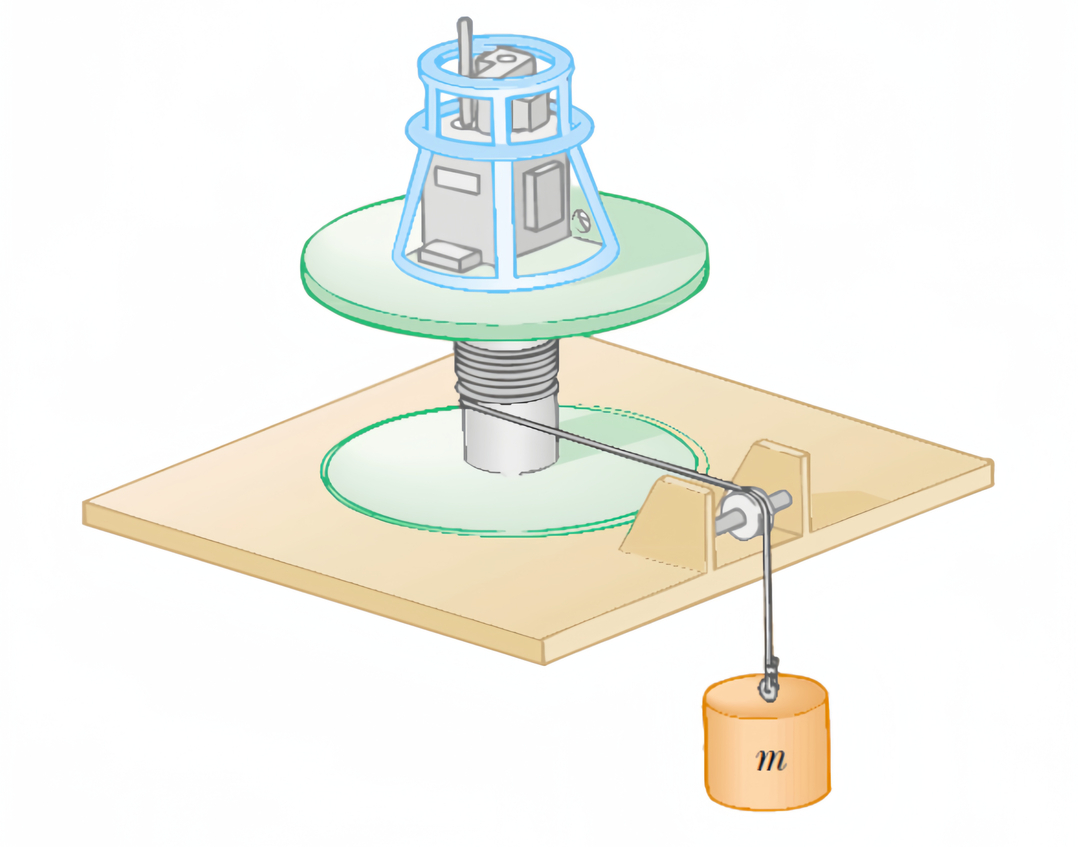
\includegraphics[width=0.6\textwidth]{chapter3_example_1}
	\end{center}
	
	这是一道基础的转动力学题目,一般的求解思路为:列力学方程---列运动方程---列关联方程---求解。
	
	设绳子的张力为$\vec{T}$,物体的转动惯量为$I$,有:
	\[\left\{
		\begin{array}{cc}
			\left.\begin{array}{c}
				Tr=I\alpha\\
				mg-T=ma
			\end{array}\right\}&\cdots\text{力学方程}\\
			v^2=2ah&\cdots\text{运动方程}\\
			a=r\alpha&\cdots\text{关联方程}
		\end{array}
		\right.\]
	联立求解即得\[I=mr^2(\dfrac{2gh}{v^2}-1)\]
\end{solution}
\begin{solution}[{\large\color{plainred}Rolling Items}\\
	Three objects of \itr{uniform density}{均匀的密度} --- a \itr{solid sphere}{实心球}, a \itr{solid
		cylinder}{实心圆柱}, and a \itr{hollow cylinder}{空心圆柱} --- are placed at the top of
	an \itr{incline}{斜坡}. \\
	If they all are released from rest
	at the same \itr{elevation}{高度} and roll without \itr{slipping}{滑动}, which object reaches the bottom first?
	]
	\begin{center}
		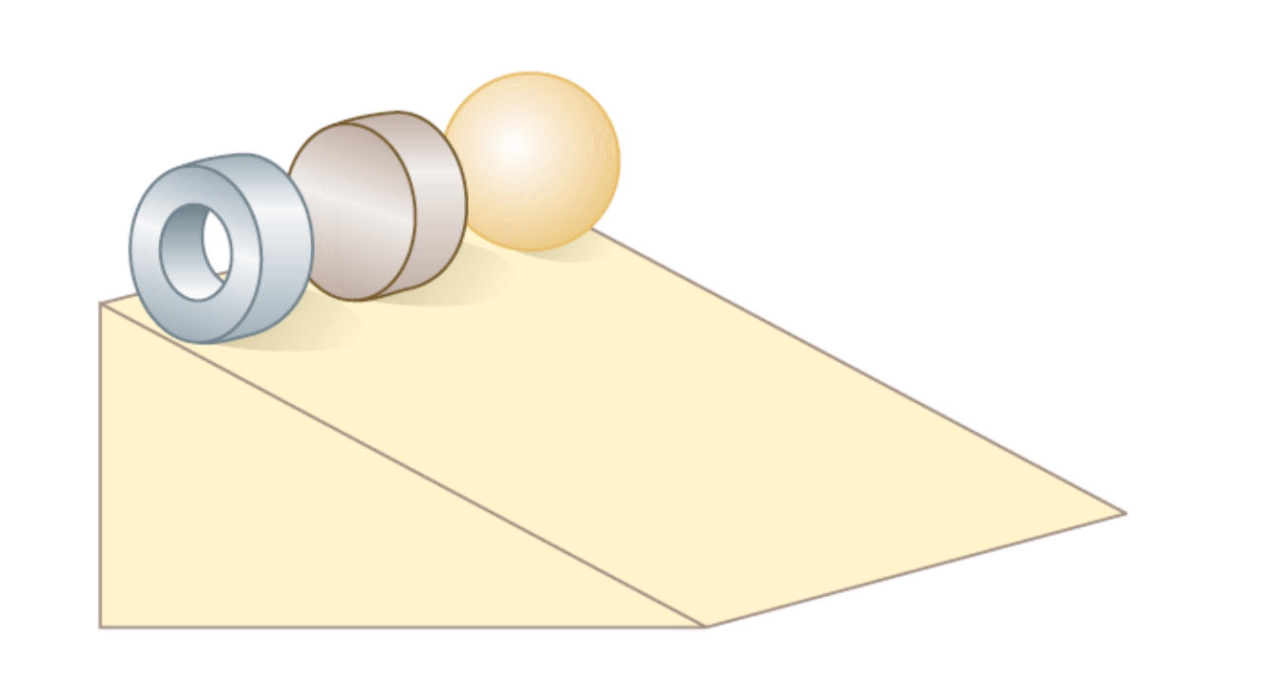
\includegraphics[width=0.6\textwidth]{chapter3_example_2}
	\end{center}
	
	本题是经典的纯滚动问题。所谓纯滚动,就是滚动体与接触面接触的点速度为$\vec{0}$(即旋转速度和质心速度相抵消)。
	%分析纯滚动时,我们往往以接触线为转动轴,以避免引入非惯性系,将问题复杂化。
	
	我们往往选择过质心的轴作为旋转轴,建立参考系。这是因为,即使这样建立的参考系是一个非惯性系,只要它不发生转动,那么,使用证明“均匀重力场中重力可以等效作用在质心”中用到的方法(\refleaftext{prove3.7}),就可以证明惯性力可以等效作用在质心。由于我们选择的是质心轴,惯性力产生的力矩恒为$0$,因此也就不会对转动的分析产生影响\footnote{很多解析都直接选择了一个非惯性质心系来分析转动,却并没有讲解惯性力可以忽略的原因。}。
	
	现在,让我们选择质心系分析问题\footnote{当然,过质心的轴有很多,但是大家应该能意会到选择了怎样的轴(对称性好的轴),就不再描述了}。
	
	若记球体$m_1$的转动惯量为$I_1$,实心圆柱$m_2$的转动惯量为$I_2$,空心圆柱$m_3$的转动惯量为$I_3$,斜面倾角为$\theta$,则有:
	\[\left\{
		\begin{array}{l}
			m_1a_1=m_1g\sin\theta-f_1\\
			m_2a_2=m_2g\sin\theta-f_2\\
			m_3a_3=m_3g\sin\theta-f_3\\
			 f_1r_1=I_1\alpha_1\\
			 f_2r_2=I_2\alpha_2\\
			 f_3r_3=I_3\alpha_3\\
			a_1=r_1\alpha_1\\
			a_2=r_2\alpha_2\\
			a_3=r_3\alpha_3
		\end{array}
	\right.\]
	于是解得
	\[\left\{
		\begin{array}{l}
			a_1=\dfrac{m_1r_1{}^2}{I_1+m_1r_1{}^2}g\sin\theta\\[2ex]
			a_2=\dfrac{m_2r_2{}^2}{I_2+m_2r_2{}^2}g\sin\theta\\[2ex]
			a_3=\dfrac{m_3r_3{}^2}{I_3+m_3r_3{}^2}g\sin\theta
		\end{array}
	\right.\]
	由常见物体的转动惯量(见\refleaftext{chapter3_moment_inertia2})知
	\begin{align*}
		I_1&=\dfrac{2}{5}m_1r_1{}^2\\
		I_2&=\dfrac{1}{2}m_2r_2{}^2\\
		I_3&=\dfrac{1}{2}m_3(r_{3(inner)}{}^2+r_3{}^2)
	\end{align*}
	易知
	\[a_1>a_2>a_3\]
	故实心球快于实心圆柱快于空心圆柱。
\end{solution}
%\refleaf*{law3.1}[-40ex]
%\refleaf*{chapter3_moment_inertia2}[-35.6ex]
\newpage
\begin{solution}[\En{\large Calculation of the Moment of Inertia}\\A rod's \itr{linear density}{线密度} is given by $\lambda=kx$, where $x$ represents the distance from the point to the rod's center. \\
	Given the length of the rod $l$, try to calculate the moment of inertia of the rod, given the rotation axis at:\\	
	(1) Center $O$ as the $y$ axis shows.\\
	(2) One end as the $y'$ axis shows.]
	\begin{center}
		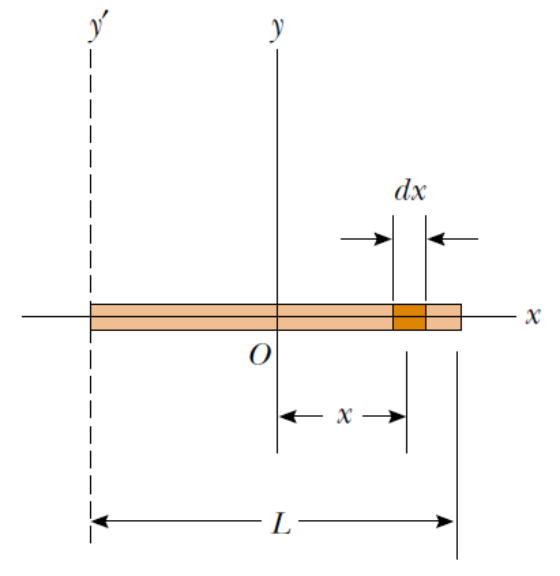
\includegraphics[width=0.5\textwidth]{chapter3_rod}
	\end{center}
	(1)由于$O$也是质心位置,不妨先求$I_{CM}$,再利用平行轴定理求解$I_{end}$。
	注意到
	\[\dif m=\lambda\dif x=k|x|\dif x\]
	于是
	\begin{align*}
		\int_{-\frac{L}{2}}^{\frac{L}{2}}(x^2)(k|x|)\dif x&=2\int_0^{\frac{L}{2}}kx^3\dif x\\
		&=2\left.(\dfrac{1}{4}kx^4)\right|_0^{\frac{L}{2}}\\
		&=\dfrac{1}{32}kL^4
	\end{align*}
	
	(2)欲用平行轴定理(\refleaftext{law3.1}),则需知晓棍子的质量。
	\begin{align*}
		m&=\int_{-\frac{L}{2}}^{\frac{L}{2}}k|x|\dif x\\
		&=2\int_0^{\frac{L}{2}}kx\dif x\\
		&=2\left.(\dfrac{1}{2}kx^2)\right|_0^{\frac{L}{2}}\\
		&=\dfrac{1}{4}kL^2
	\end{align*}
	故
	\[I_{end}=I_{CM}+m(\dfrac{L}{2})^2=\dfrac{3}{32}kL^4\]
\end{solution}
\begin{solution}[\En{\large Massive \itr{Pulley}{滑轮}}\\Consider two \itr{cylinders}{圆柱} having masses $m_1$
	and $m_2$, where $m_1 < m_2$, connected by a
	string passing over a pulley. The pulley
	has a radius $R$ and moment of inertia $I$
	about its axis of rotation. The string does
	not \itr{slip}{滑动} on the pulley, and the system
	is released from rest. Find the linear
	speeds of the cylinders after
	cylinder 2 \itr{descends}{下降} through a
	distance $h$, and the angular
	speed $\omega$ of the pulley at this time.]
	\begin{center}
		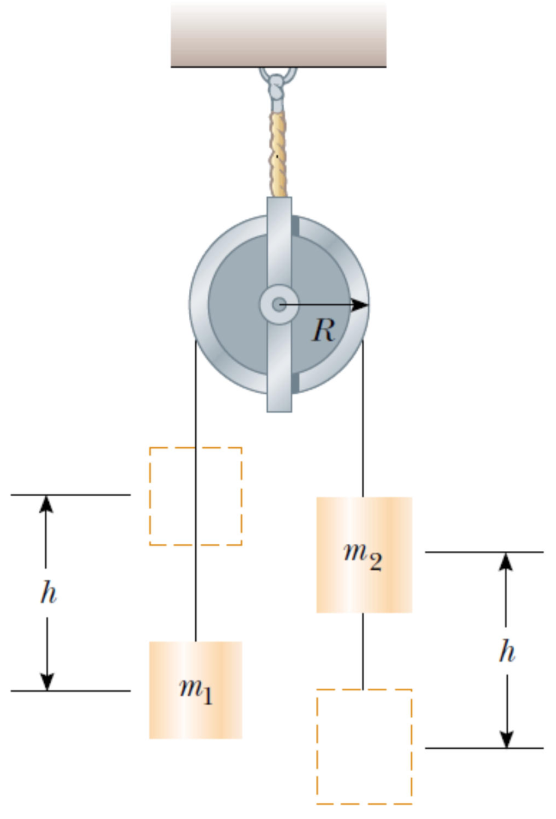
\includegraphics[width=0.3\textwidth]{chapter3_massive_pulley}
	\end{center}
	本题可从运动角度或能量角度考虑。\\
	法一:运动分析\\
	设左绳的张力为$T_1$,右绳的张力为$T_2$,则有
	\[\left\{\begin{array}{c}
		T_1-m_1g=m_1a\\
		T_2R-T_1R=I\alpha\\
		m_2g-T_2=m_2a\\
		a=R\alpha
	\end{array}\right.\]
	于是解得
	\[a=\dfrac{m_2-m_1}{m_1+m_2+\frac{I}{R^2}}g\]
	则
	\[v=\sqrt{2ah}=\sqrt{\dfrac{m_2-m_1}{m_1+m_2+\frac{I}{R^2}}2gh},\quad\omega=\sqrt{\dfrac{m_2-m_1}{(m_1+m_2)R^2+I}2gh}\]
	法二:能量分析\\
	系统机械能守恒,于是有
	\[\left\{\begin{array}{c}
		m_2gh=m_1gh+\dfrac{1}{2}m_1v^2+\dfrac{1}{2}m_2v^2+\dfrac{1}{2}I\omega^2\\
		v=R\omega
	\end{array}\right.\]
	亦可解得
	\[v=\sqrt{2ah}=\sqrt{\dfrac{m_2-m_1}{m_1+m_2+\frac{I}{R^2}}2gh},\quad\omega=\sqrt{\dfrac{m_2-m_1}{(m_1+m_2)R^2+I}2gh}\]
\end{solution}
\begin{solution}[\En{\large Object rotating on a string
		of changing length}\\Initially, the mass \itr{revolves}{转动} with a speed $v_1$ = 2.4 m/s in
		a circle of radius $R_1$ = 0.80 m.
		The string is then pulled slowly through the hole so
		that the radius is reduced to $R_2$ = 0.48 m. What is the
		speed, $v_2$, of the mass now?]
	\begin{center}
		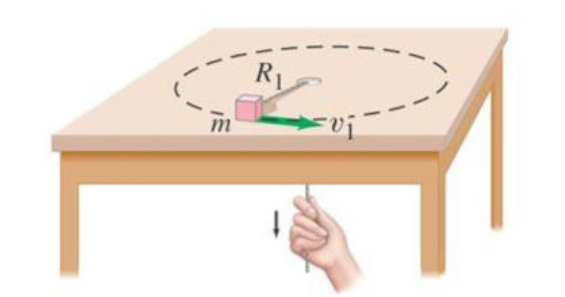
\includegraphics[width=0.7\textwidth]{chapter3_string}
	\end{center}
	本题考察角动量守恒。可以注意到,绳子对物块的力始终是径向的,对应的力矩始终为$\vec{0}$,因此,物块的角动量守恒。不妨就以洞为轴,有
	\[I_1\omega_1=I_2\omega_2\Rightarrow R_1{}^2\omega_1=R_2{}^2\omega_2\]
	代入$\omega_1=\dfrac{v_1}{R_1},\quad\omega_2=\dfrac{v_2}{R_2}$,即得
	\[v_1R_1=v_2R_2\]
	代入数据即得$v_2=4.0$m/s.
\end{solution}
\begin{solution}[\En{\large Rotation of a sliding rigid rod}\\Consider a rod with mass m and length L standing straight on the friction-less ground. When we
	release the rod, it will fall from the unstable \itr{equilibrium position}{平衡位置}\!.\\
	(a) Calculate the angular velocity of the rod, when it has an angle of $\theta$ with respect to the ground
	as illustrated in Figure 1.\\
	(b) What is the final angular velocity $\omega_1$ of the rod before it hits the ground?\\
	(c) If the same rod is leaning to a frictionless wall with an initial angle of α to the frictionless
	ground (see Figure 2), what is the final angular velocity $\omega_2$ of the rod before it hits the ground?\\
	{\em Note that there is a possibility that the right end of the rod leaves from the wall before the rod hits the ground.}]
	\begin{center}
		\begin{minipage}{0.45\textwidth}
			\centering
			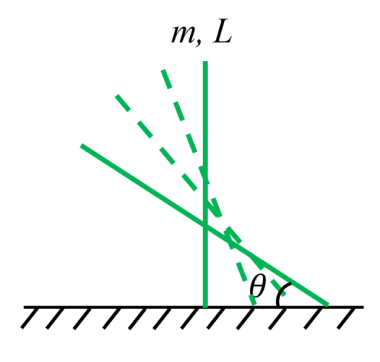
\includegraphics[width=\linewidth]{chapter3_rotating_rod_1}\\
			Figure 1
		\end{minipage}
		\quad
		\begin{minipage}{0.45\textwidth}
			\centering
			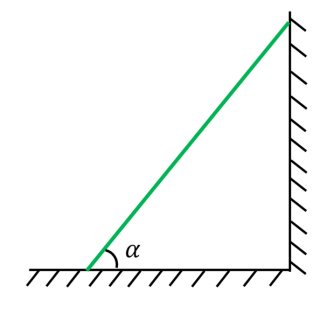
\includegraphics[width=\linewidth]{chapter3_rotating_rod_2}\\
			Figure 2
		\end{minipage}
	\end{center}
	本题主要考察转动中的能量守恒,以及对平动速度和角速度关系的分析。
	
	(a) 首先,由题意知不存在摩擦力,而支持力做功始终为零,所以以棍子为研究对象,有机械能守恒。又注意到,棍子在水平方向始终不受力,因此质心是在垂直下降。于是有
	\begin{equation}
		mg\dfrac{L}{2}-mg\dfrac{L}{2}\sin\theta=\dfrac{1}{2}mv_{CM}{}^2+\dfrac{1}{2}I\omega^2
	\end{equation}
	研究质心的运动,有
	\begin{align}
		v_{CM}&=\dfrac{\dif (\frac{L}{2}\sin\theta)}{\dif t}\\[1ex]
		&=\dfrac{L}{2}\dfrac{\dif\sin\theta}{\dif\theta}\dfrac{\dif\theta}{\dif t}\\[1ex]
		&=\dfrac{L}{2}\cos\theta\omega
	\end{align}
	将(3.4)代入(3.1)即得
	\begin{equation}
		\omega=2\sqrt{\dfrac{3g}{L}\dfrac{1-\sin\theta}{1+3\cos^2\theta}}
	\end{equation}
	(b) 即考虑(a)中的极限情况,将$\theta=0$代入(3.5)中即得
	\begin{equation}
		\omega_1=\sqrt{\dfrac{3g}{L}}
	\end{equation}
	(c) \begin{center}
		\begin{tikzpicture}[scale=2]
			\coordinate (O) at (0,0);  
			\coordinate (A) at (-1,0);  
			\coordinate (B) at (0,1.732); 
			\coordinate (D) at (-1.5,0);
			\coordinate (E) at (0,2.5); 
			\coordinate (BB) at (0,1.414);
			\coordinate (AA) at (-1.414,0);
			
			\draw [green](A) -- (B) ; 
			\draw [thick=3pt](D)--(O);
			\draw [thick=3pt](O)--(E);
			\draw [green,dashed](AA)--(BB);
			
			\coordinate (M) at ($(A)!0.5!(B)$);  
			\coordinate (N) at ($(AA)!0.5!(BB)$);
			
			\draw[dashed,plainred] (O) -- (M);  
			\draw[dashed,plainred] (O)--(N);
			\draw[dashed,yellow5] (0,0) circle[radius=1];
			
			\node[below left] at (A) {$A$};  
			\node[above right] at (B) {$B$};  
			\node[above right] at (BB) {$B'$};
			\node[below left] at(AA) {$A'$};
			\node[above left] at (M) {$C$};  
			\node[below left] at (O) {$O$};  
			\node[above right]at (A) {$\ \ \ \alpha$};
			\node[above left] at (N) {$C'$};
			\draw (-0.8,0) arc(0:60:0.2);
			\draw (-1.214,0) arc (0:45:0.2);
			\node[above right] at (AA) {$\ \ \ \,\theta$};
		\end{tikzpicture}  
	\end{center}
		
如图,先考虑棍未与墙壁脱离情形,注意到质心$C$到$O$的距离始终为$\dfrac{L}{2}$,因此确定质心的运动轨迹是一个圆。由$\angle COA=\angle CAO$,知$v_{CM}=\omega\dfrac{L}{2}$,即关系式。再由\\[1ex]“无摩擦力”,“支持力不做功”知棍子机械能守恒,于是可以列出守恒式:
		\begin{equation}
			mg(\dfrac{L}{2}\sin\alpha-\dfrac{L}{2}\sin\theta)=\dfrac{1}{2}mv_{CM}{}^2+\dfrac{1}{2}I\omega^2
		\end{equation}
由(3.7)可解得
\begin{equation}
	\omega=\sqrt{\dfrac{3g(\sin\alpha-\sin\theta)}{L}}
\end{equation}
接下来,我们考虑临界条件。当棍子脱离墙时,来自墙的支持力消失,也就是说,\textbf{质心在水平方向不再拥有加速度}。于是,$v_{CMx}$最大时,棍子将脱离墙。
\begin{align}
	v_{CMx}&=v_{CM}\sin\theta\\
	&=\omega\dfrac{L}{2}\sin\theta\\
	&=\dfrac{\sin\theta}{2}\sqrt{3gL(\sin\alpha-\sin\theta)}\\
	&=\sqrt{3gL}\cdot\sqrt{\dfrac{\sin\theta}{2}}\cdot\sqrt{\dfrac{\sin\theta}{2}}\cdot\sqrt{\sin\alpha-\sin\theta}\\
	&\le\dfrac{1}{3}\sin\alpha\sqrt{gL\sin\alpha}\quad(\text{当且仅当}\sin\theta=\dfrac{2}{3}\sin\alpha)
\end{align}
之后,在水平方向,质心的运动保持不变。由(3.4)知,当棍子即将落地时,有\begin{equation}
	v_{CMy}=\dfrac{L}{2}\omega_2
\end{equation}于是可以列守恒式
\begin{equation}
	mg\dfrac{L}{2}\sin\alpha=\dfrac{1}{2}m(v_{CMx}{}^2+v_{CMy}{}^2)+\dfrac{1}{2}I\omega_2{}^2
\end{equation}
将(3.14)代入(3.15)即得
\begin{equation}
	\omega_2=\sqrt{(9\sin\alpha-\sin^3\alpha)\dfrac{g}{3L}}
\end{equation}
\dove\ PS:这大概是本章考察的天花板了。
\end{solution}

\chapter[流体力学]{\itr{Fluid Mechanics}{流体力学}}
\begin{solution}[流体静力学]
    A fluid is rotating at constant angular velocity $\omega$ about the central vertical axis of a cylindrical container.As shown in Figure 4-1:
    \begin{singlefigure}[流体静力学]{chapter4_流体静力学}[0.45]
    \end{singlefigure}

    (a) Show that the \itr{variation}{变化} of pressure in the \itr{radial direction}{径向} is given by $\dfrac{\dif p}{\dif r}=\rho \omega^2 r$.

    (b) Take $p=p_c$ at the axis of rotation ($r=0$) and show that the pressure $p$ at any point $r$ is
    \begin{center}
        $p=p_c+\dfrac{1}{2}\rho\omega^2 r^2$
    \end{center}

    (c) Show that the liquid surface is of \itr{paraboloidal}{抛物面的} form(Figure 4-1); that is, a vertical cross section of the surface is the curve $y=\dfrac{\omega^2 r^2}{2g}$.

    \tcbrule

    (a)取一段竖直方向的薄平面,设其截面积为A,沿半径方向的厚度为$\dif r$,深度为$h$。如下图所示:
    \begin{singlefigure}[A-4-1]{chapter4_E1_A1}[0.45]
    \end{singlefigure}

    可知水平方向的压强差为$\dif p=p_{r+\dif r}(h)-p_r(h)$,其中$p=p_0+\rho gh$。由受力关系结合匀速圆周运动可得:
    \[F=A\dif p=A\dif r \rho \omega^2 r\]
    整理得到(a)中的公式。

    (b)化简上式并积分:
    \[\int_{p_{h,0}}^{p_{h,r}}\dif p=\int_{0}^{r}\rho \omega^2 r\dif r\]

    得到:$p=p_0+\rho gh+\dfrac{\rho \omega^2 r^2}{2}$。其中前两项与半径无关,即为$p_c$,可得:
    \[p=p_c+\dfrac{1}{2}\rho \omega^2 r^2\]

    (c)液体表面的压强均为大气压强,将$p=p_0$、$p_c=p_0+\rho gh$代入(b)中得到的公式,得:
    \[\rho gh+\dfrac{1}{2}\rho \omega^2 r^2=0\]
    由于深度的坐标轴是向下的,我们以页面最低点处的水平方向为r轴,沿中心线竖直方向作为y轴,也就是调转一下坐标系。应用上述公式可知:
    \[y=\dfrac{\omega^2 r^2}{2g}\]
\end{solution}

\begin{solution}[流体动力学]
    As shown in Figure 4-3, it is an \itr{air suction device}{空吸装置}. Given that the depth of the centerline of the \itr{catheter}{导管} below the liquid level in container $A$ is $h$,
    the height difference between the liquid level in container $B$ and the centerline of the horizontal catheter is $h_b$, \itr{the cross-sectional area}{横截面积} at the \itr{nozzle}{喷嘴} $d$ is $S_d$,
    and the cross-sectional area at the \itr{contraction section}{收缩段} $c$ is $S_c$. What are the conditions for the \itr{ratio}{比率} of $S_d$ to $S_c$ to occur for \itr{suction}{抽吸}?
    \begin{singlefigure}[流体动力学]{chapter4_流体动力学}[0.65]
    \end{singlefigure}

    \tcbrule

    取一个流线Acd,对c、d两点应用伯努利公式可得:
    \[\dfrac{1}{2}\rho v_c^2+p_c=\dfrac{1}{2}\rho v_d^2+p_d\]
    其中d点的流速为$v_d=\sqrt{2gh}$,气压为大气压强$p_d=p_0$。且由于连续性原理,有:
    \[v_c S_c=v_d S_d\]
    因此c、d两点的压强差为:
    \[p_c-p_0=\rho gh(1-(\dfrac{S_d}{S_c})^2)\]
    而容器B液面的压强也是大气压强。发生空吸作用只要满足条件:
    \[p_c<p_0-\rho gh_b\]
    代入公式即可得到:
    \[\dfrac{S_d}{S_c}>\sqrt{1+(\dfrac{h_b}{h})}\]
\end{solution}
\chapter{title}
\chapter[狭义相对论]{\itr{Special relativity}{狭义相对论}}
\begin{solution}[{\large\color{plainred}Fizeau effect}\\In this problem we show that the relativistic velocity addition law can be used to
	explain the Fizeau experiment without invoking the existence of \itr{ether}{以太}. The speed of light in stationary water is less than its speed $c$ in \itr{vacuum}{真空}.
	Traditionally it is written as $\frac{c}{n}$, where $n\approx \frac{4}{3}$ is the \itr{index of refraction}{折射率} of water. The water flowed in the \itr{pipe}{管道} with
	velocity $v$. In the lower arm $T_2$ of the \itr{interferometer}{干涉仪} (as shown in the figure), one would expect that, from the nonrelativistic addition law, the
	speed of light in the moving water would be its speed in stationary
	water increased by the speed of the water in the pipe $w=\frac{c}{n}+v$. Show
	that the relativistic velocity addition law leads to, up to higher-order
	corrections:
	\begin{equation*}
		w=\frac cn+v\left(1-\frac1{n^2}\right)
	\end{equation*}
	The result was observed by Fizeau in 1851, but for long time viewed as
	a confirmation of a rather \itr{elaborate}{复杂的} \itr{contemporary}{同时代的} ether-theoretical
	calculation based on the idea that the water was partially successful in
	dragging ether along with it. Einstein later said that it was of
	fundamental importance in his thinking.]
      \begin{center}
      	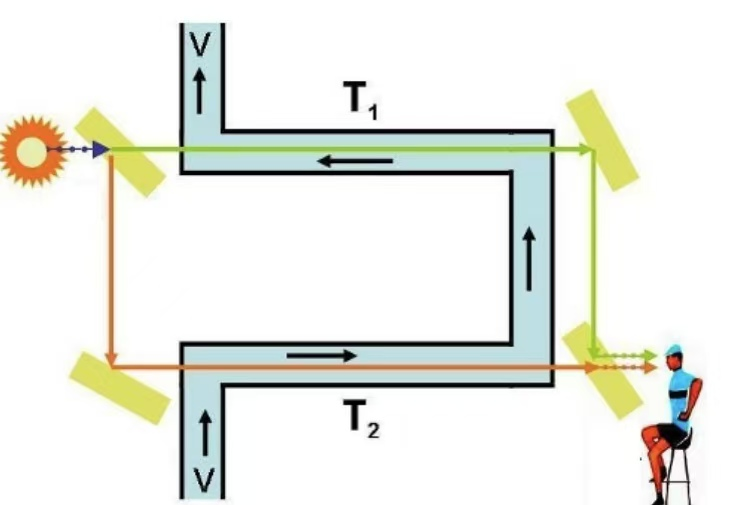
\includegraphics[width=5.5cm, height=4cm]{chapter_6_7}
      \end{center}
      此类题目主要是要选取恰当的参考系,并列出对应参数。
      
      以地面为$S$系,水流为$S^{\prime}$系,并设光前进方向为$x$轴正方向。
      
      在$S$系中,静止的水中光速为$\dfrac{c}{n}$,下方水的速度即$S^{\prime}$系相对$S$系的速度为$v$
      
      那么在$S^{\prime}$系中,由速度变换
      
      \[w=\dfrac{\dfrac{c}{n}+v}{1+\dfrac{cv}{nc^{2}}}=\dfrac{\dfrac{c}{n}+v}{1+\dfrac{v}{nc}}\]
      
      注意到$v\ll c$,故$\dfrac{v}{nc}$为小量,利用泰勒展开至一阶:
      \begin{equation*}
      	\dfrac{1}{1+\dfrac{v}{nc}} = 1 - \dfrac{v}{nc} + o\left(v^{2}\right) 
      \end{equation*}
      代入表达式中,并忽略$v^{2}$相关的高阶小量,即有:
      \[w\approx(\frac{c}{n}+v)(1-\frac{v}{nc})=\frac{c}{n}+v(1-\frac{1}{n^{2}})\]
\end{solution}
\begin{solution}[{\large\itr{Terrel Rotation}{特雷尔旋转}}\\  A square with proper-length-$L$ sides flies past you at a speed $v$, in a direction parallel to two of its sides. You stand in the plane of the square. When you see the square at its nearest point to you, show that it looks to you like it is rotated, instead of contracted. (Assume that $L$ is small compared with the distance between you and the square.)]
    \itr{Terrel Rotation}{特雷尔旋转} 是相对论效应之一,即当物体以接近光速运动时,观察者会看到物体在视觉上旋转。
    
    \ctikzfig{chapter6_solution_6_2_2}
    首先,正如图中标明的,由于尺缩效应,与运动同向的边$AB,CD$在$O$系中长度缩短为$sL$。
    
    之后,注意到我们处理的是视觉效应,那么我们就要考虑光信号到达人眼中才能成像的问题。举边$AD$为例,边上的每一个点发出的光到达人眼的时间都是不同的。在这里,我们考虑$A,D$两点。
    
    连接$AO,DO$,由于题目条件中说,人与正方形的距离远远大于$L$,可以认为$D,A,O$\\[1ex]
    近似成一条直线。因此,$A$发出的光比$D$发出的光提前$\dfrac{L}{c}$的时间到达人眼。\\[1ex]
    换而言之,人眼中接受的光信号,其实是某个时刻的$A$发出的信号,以及该时刻前\\[1ex]
    $\dfrac{L}{c}$的时刻时$D$发出的信号。人眼同时处理这两个信号,产生了“观察到$DA$边”的\\[1ex]
    效果。
    
    \ctikzfig{chapter6_solution_6_2_3}
    
    这张图中的$D_v-A_v-B_v$显示了人眼中观察到的现象。$A_vB_v$的长度即由于尺缩效\\[1ex]
    应得到的$sL$,而$A_vD_v$的长度则等于光信号时间差$\dfrac{L}{c}$乘以正方形运动的速度$v$,也\\[1ex]
    即$\beta L$。
    
    这里我们发现,恰有$(\beta L)^2 + (sL)^2 = L^2$。因此,人眼所看见的,就好像是图中旋转后的正方形$ABCD$在运动方向的投影。且对于旋转的角度$\theta$,有
    \[\sin\theta=\dfrac{\beta L}{L}=\beta\]
\end{solution}
\begin{solution}[{\large\color{plainred}Lots of transformations}\\A train with proper length $L$ moves at speed $\dfrac{c}{2}$ with respect to the ground. A ball is thrown from the back to the front, at speed $\dfrac{c}{3}$ with respect to the train. How much time does this take, and what distance does the ball cover, in:
	\\(a) The train frame?
	\\(b)The ground frame? Solve this by:
	\\\hspace*{2em}i. Using a velocity-addition argument.
	\\\hspace*{2em}ii. Using the Lorentz transformations to go from the train
	frame to the ground frame.
	\\(c)The ball frame?
	\\(d) Verify that the \itr{invariant interval}{不变(时空)间隔} is indeed the same in all three
	frames.]
         \begin{singlefigure}{chapter_6_19}[0.6]        
        \end{singlefigure}
        (a)火车相对自身是静止的,故火车系下其长度就是原长,而火车系下球的速度已知,故有
        \begin{equation*}
        	\begin{aligned}
        		&\Delta x_{1}=L\\
        		&\Delta t_{1}=\frac{L}{c/3}=\frac{3L}{c} \\
        	\end{aligned}
        \end{equation*}
        (b)选取地面为$S$系,火车为$S^{\prime}$系,火车前进方向为$x$正方向。$S^{\prime}$系相对$S$系的速度$u$为
        \[u=\dfrac{c}{2}\]
        (i)$S^{\prime}$系中球的速度为$v^{\prime}=\dfrac{c}{3}$,由速度变换公式有$S$系中,球的速度
        \[v=\dfrac{v^{\prime}+u}{1+\dfrac{{v}^{\prime}u}{c^2}}=\frac{5c}{7}\]
        列车在地面看来会发生尺缩效应,且尺缩因子$s = \sqrt{1-\left(\dfrac{u}{c}\right)^{2}} = \dfrac{\sqrt{3}}{2}$,得地面系中列车长度
        \[ d=sL = \dfrac{\sqrt{3}}{2}L\]
        在$S$系中是一个追及问题,所需时间:
        \[\Delta t_2=\frac{d}{v-u}=\frac{7\sqrt{3}L}{3c}\]
        所走距离
        \[\Delta x_2=vt_{2}=\frac{5\sqrt{3}L}{3}\]
        (ii)利用洛伦兹变换的变化量形式:
        \begin{equation*}
        	\begin{aligned}
        		&\Delta t_2 = \gamma(\Delta t_1 + \frac{u} {c^{2}}\Delta x_1)\\
        		&\Delta x_2 = \gamma(\Delta x_1 + u\Delta t_1)
        	\end{aligned}
        \end{equation*}
        可求得
        \begin{equation*}
        	\begin{aligned}
        		&\Delta t_2=\frac{7\sqrt{3}L}{3c}\\[1ex]
        		&\Delta x_2=\frac{5\sqrt{3}L}{3}\\
        	\end{aligned}
        \end{equation*}
        
        (c)在设球参考系为$S^{\prime \prime}$系,显然$S^{\prime \prime}$系下球是静止的:
        \begin{equation*}
        	\Delta x_3=0
        \end{equation*}   
        $S^{\prime \prime}$系相对$S^{\prime}$系速度$u^{\prime} = \dfrac{c}{3}$,
        有$\gamma^{\prime} = \dfrac{1}{\sqrt{1-\left(\dfrac{u^{\prime}}{c}\right)^{2}}} = \dfrac{3\sqrt{2}}{4}$,利用洛伦兹变换得
        \begin{equation*}
        	\Delta t_{3}= \gamma^{\prime}(\Delta t_1 - \frac{u^{\prime}\Delta x_1} {c^{2}})
        	=\frac{2\sqrt{2}L}{c}
        \end{equation*}
        
        (d)题意其实就是要证明时空间隔$(c\Delta t)^2-(\Delta x)^2$的不变性,将之前所求代入验证即可:
        \begin{equation*}
        	\begin{aligned}
        		(c\Delta t_{1})^{2}-(\Delta x_{1})^{2}&=8L^{2} \\
        		(c\Delta t_{2})^{2}-(\Delta x_{2})^{2}&=8L^{2}\\
        		(c\Delta t_{3})^{2}-(\Delta x_{3})^{2}&=8L^{2} \\
        	\end{aligned}
        \end{equation*}
        可见事件的时空间隔确实不变。
        
        注:如果老师上课时定义的时空间隔与此处不同,注意符号问题或者在回答时说明好。
\end{solution}
\begin{solution}[{\large\color{plainred}Train And \itr{Tunnel}{隧道} \itr{Paradox}{悖论}}\\
	Consider a train running at a constant speed $V$ on the straight track in the $x$ direction, and passing through a tunnel (see the figure). The proper length of the train is $L$, and the proper length of the tunnel is $D$. Here we assume $L>D$. Define $(x,ct)$ as the time and the space coordinates of the track frame, and $(x',ct')$ as those of the train frame. Here, $x$ and $x' $\textbf{ are in the same direction}.	
	\\
	(a) Suppose that an observer standing on the ground sees that the train is shorter than the tunnel, so that the whole train can be inside the tunnel. Determine the smallest possible speed of the train.
	\\
	(b) Suppose that the rear end of the tunnel (see the figure) is at $x=0$, and set the time $t=t'=0$ when the rear end of the train reaches the rear end of the tunnel. Draw the Minkowski diagram \textbf{ taking $x$ coordinate for the horizontal axis and $ct$ coordinate for the vertical axis.} In addition, \itr{specify}{指明} $L$ and $D$ in the diagram.
	\\
	(c) When the rear end of the train enters the rear end of the tunnel, the rear-end and front-end sliding doors of the tunnel (see the figure) are closed at the same time in the track frame. These two events are denoted by $R_{close}$ and $F_{close}$, respectevely. Then, when the front-end of the train reaches the front end of the tunnel, both the rear-end and front-end sliding doors are opened at the same time in the track frame. These events are denoted by $R_{open}$ and $F_{open}$, respectively.
	\\
	Show the events $R_{close},F_{close},R_{open}$, and $F_{open}$ in the Minkowski diagram in (b),
	and put the four events in the order of being seen by an observer in the train.
	]
	\begin{singlefigure}{chapter_6_20}[1]    
	\end{singlefigure}
    (a)
    \\根据尺缩效应,在轨道参考系中,火车的长度为
    \[\sqrt{1-\dfrac{v^2}{c^2}}L\]
    故如需火车能够完全在隧道中,则有
    \[\sqrt{1-\dfrac{v^2}{c^2}}L\le D\]
    可解得
    \[v\ge \sqrt{1-\dfrac{D^2}{L^2}}c\]
    (b)\\
    作图如下:
    \begin{center}
    	\resizebox{16.2em}{12em}{\tikzfig{chapter6_solution_6_4_1}}
    \end{center}
    
    
    依据题意,隧道尾和火车尾在$0$时刻都处于$O$点。由于隧道在轨道系中静止,隧道在轨道系中的长度即为其原长$D$。因此,在$x$轴上取长度$D$,对应的$P$点即是$0$时刻时隧道头的位置。
    
    首先,需要过$P$做校准曲线,与$x'$轴相交于$Q_1$点。由于题目条件$L>D$,因此$L$的端点在$Q_1$右侧。
    
    另外,还需要过$P$作$ct'$轴的平行线,交$x'$轴于$Q_2$点。这是因为列车在轨道系(也就是$x-ct$系)中的长度应当小于$D$,且列车头的世界线斜率与$ct'$轴斜率相同。于是,过$L$的端点作$ct'$轴的平行线与$x$轴的交点应在$P$的左侧,等价于$L$的端点在$Q_2$的左侧。
    
    综上,任取一点在$Q_1,Q_2$之间,它与$O$的距离就可以表示$L$。
    (c)\\
    根据题意作出图如下
    \begin{singlefigure}{chapter_6_22}[0.6]   
    \end{singlefigure}
    作出平行线后发现
    \[{t_1}^{\prime}<{t_2}^{\prime}<{t_3}^{\prime}<{t_4}^{\prime}\]
    故有
    \[F_{close}\rightarrow F_{open}\rightarrow R_{close}\rightarrow R_{open}\]
\end{solution}
\begin{solution}[{\large\color{plainred}Conservation of momentum in SR}]
      (i)由速度变换 
        \[v^{\prime}=\frac{v+v}{1+\frac{v^{2}}{c^{2}}}=\frac{2v}{1+\frac{v^{2}}{c^{2}}} \]
      (ii)对于红色粒子
        \[v_{xr}=0\]
        \[v_{yr}=\frac{v\sqrt{1-\beta^{2}}}{1+\frac{0v}{c^{2}}}=v\sqrt{1-\frac{v^{2}}{c^{2}}}\] 
        对于蓝色粒子
        \[v_{xb}=v\] 
        \[v_{yb}=\frac{-v\sqrt{1-\beta^{2}}}{1+\frac{0v}{c^{2}}}=-v\sqrt{1-\frac{v^{2}}{c^{2}}} \]
     (iii)在$k^{\prime}$系下\\
         碰前动量
        \[\overrightarrow{P_{0}}=\frac{mv^{\prime}}{\sqrt{1-(\beta^{\prime})^{2}}}\overrightarrow{i},\beta^{\prime}=\frac{v^{\prime}}{c}=\frac{2\beta}{1+\beta^{2}}\]
        代入发现
        \[P_{0}=\frac{2mv}{1-\beta^{2}}\overrightarrow{i}\]
        碰后动量
        \[\overrightarrow{P}=\frac{2mv}{\sqrt{1-(\beta^{\prime\prime})^{2}}}\overrightarrow{i}\]
        注意此时
        \[\beta^{\prime\prime}=\frac{\sqrt{v_x^{2}+v_y^{2}}}{c}\]
        故$\beta^{\prime\prime}=\beta\sqrt{2-\beta^{2}}$\\
        代入后有
        \[\overrightarrow{P}=\frac{2mv}{1-\beta^{2}}\overrightarrow{i}\]
        故$\overrightarrow{P}=\overrightarrow{P_{0}}$,动量守恒

\end{solution}
\begin{solution}[{\large\color{plainred}Perfectly Inelastic Collison of two Relastivistic Particles}]
    (a) 由能量守恒
    \[\frac{mc^2}{\sqrt{1-\frac{v^2}{c^2}}}=Mc^2\]
    故$M=\frac{m}{\sqrt{1-\frac{u^{2}}{c^{2}}}}$
    (b)由速度变换
    \[u=\frac{v+v}{1+\frac{v^{2}}{c^{2}}}=\frac{2v}{1+\frac{v^{2}}{c^{2}}}\]
    (c)碰前动量
    \[P_{0}=\frac{mu}{\sqrt{1-\frac{u^{2}}{c^{2}}}}=\frac{2mu}{1-\frac{v^{2}}{r^{2}}}\]
    碰后动量
    \[P=\frac{2Mv}{\sqrt{1-\frac{v^{2}}{c^{2}}}}=\frac{2mv}{1-\frac{v^{2}}{c^{2}}}\] 
    $P=P_0$,故动量守恒\\
    碰前能量 
    \[E_{0}=mc^{2}+\frac{mc^{2}}{\sqrt{1-\frac{u^{2}}{c^{2}}}}=\frac{2mc^{2}}{1-\beta^{2}}\]
    碰后能量
    \[E=2\frac{Mc^{2}}{\sqrt{1-\frac{v^{2}}{c^{2}}}}=\frac{2mc^{2}}{1-\beta^{2}}\]
    $E=E_0$,故能量守恒。
\end{solution}
\begin{solution}[{\large\color{plainred}Relastivistic Scattering between a Photon and an Electron}]
(a)\\   
    (i)\[E=\frac{mc^{2}}{\sqrt{1-\frac{1}{t^{2}}}},\mathbf{P}=\frac{m\mathbf{v}}{\sqrt{1-\frac{v^2}{c^{2}}}}\]
    (ii)由速度变换
    \[v^{\prime}=\frac{v-u}{1-\frac{uv}{c^2}}=\frac{\beta_{v}-\beta_{u}}{1-\beta_{u}\beta_{v}}\]
    又$\gamma^{\prime}=\frac{1}{\sqrt{1-\frac{{v^{\prime}}^{2}}{c^{2}}}}$
    故有
    \[\frac{1}{{\gamma^{\prime}}^{2}}=\frac{1}{\gamma^{2}}\frac{1}{\gamma_{u}^{2}}(1-\beta_{u}\beta_{v})^{2}\]
    即$\gamma^{\prime}=\frac{\gamma_{u}\gamma}{1-\beta_{u}\beta_{v}}$
    故$\frac{E^{\prime}}{c}=\gamma^{\prime}\frac{mc^{2}}{c}=(\frac{E}{c}-\frac{|\mathbf{P|}u}{c})\gamma_{u}$
    \[\mathbf{P^{\prime}}|=(|\mathbf{P}|-\frac{uE}{c^{2}})\gamma_{u}\]
(b)\\
(i) \[\mathbf {P}\cdot \mathbf{P}= \frac {E^{2}}{c^{2}}- P^{2}\]
又$E^2-p^2c^2=m^2c^4$ \\
故$\mathbf{P}\cdot\mathbf{P}=m^2c^2$\\
 (ii) 
\[{\mathbf{P}} ^{\prime }\cdot {\mathbf{P}} ^{\prime }= \frac {{E^{\prime}}^2-{p^{\prime}}^{2}c^{2}}{c^{2}}= m^{2}c^{2}= \mathbf{P} \cdot \mathbf{P}\]
(iii)\\
\[\mathbf{k}\cdot\mathbf{k}=0\]
(c)\\
换到以$u$运动系中,\\
入射前
\[\vec{P}(p,p,0,0),\vec{P}_{e}(mc,0,0,0)\]
入射后
\[\vec{P}^{\prime}(p^{\prime},-p^{\prime},0,0),\vec{P_e}^{\prime}(b_{mc},\delta_{m}v,0,0)\]
\[\vec{P}+\vec{P}_{e}=\vec{P}_{e^{\prime}}+\vec{P}^{\prime}\]
即\[\vec{P}-\vec{P}^{\prime}=\vec{P_e}^{\prime}-\vec{P_e}\]
取平方
\[\vec{P}^2+{\vec{P}^{\prime}}^2-2\vec{P}^2{\vec{P}^{\prime}}^2={\vec{P_e}^{\prime}}^2+\vec{P_e}^{2}\]
并注意到
\[\vec{P^{2}}={\vec{P^{\prime}}}^{2}=0\]
\[{\vec{{P_e}^{\prime}}}^{2}=\vec{P_e^{2}}=m^{2}c^{2}\]
故\[2\vec{P}\cdot\vec{P^\prime}=(\gamma-1)m^{2}c^{2}\]
\\又能量守恒
\[(\gamma-1)mc^{2}=pc-p^{\prime}c\]
消去$\gamma$,故
\[\frac{1}{P^{\prime}}=\frac{1}{P}+\frac{2}{mc}\]
即\[\frac{1}{E_{Ph}^{\hbar}}=\frac{1}{E_{Ph}}+\frac{1}{mc^{2}}\]
\end{solution}
\input{../chapters/chapter7/chapter7_answer}
\backmatter
\chapter{后记}
啊,终于做完了。我这辈子排过最复杂的 \LaTeX 文档恐怕就是这个了吧。

恰恰是在我生日的前一天(或者当天?),我完成了这个项目最后的收尾工作。在这学期听到王业伍老师说普物教学小组有自己编纂一本教材的想法,不知道进度怎样了,我们的项目不会白做了吧(不是)?

这是我第一次组织一个多人合作的项目。在这个过程中,我做过很多努力,也犯过一些错误,感谢愿意加入我的朋友,感谢所有的帮助与批评,正是这些让我继续成长。

我已经要进入大二下学期了,我的精力将不再支持我做普物笔记第二季了,真希望能有人能接过这个项目啊。

冬天好冷。

未来会更好的吧。

致谢:
\begin{align*}
    Ch1\quad&\text{\dove}\\
    Ch2\quad&\text{刘远鉴}\\
    Ch3\quad&\text{\dove}\\
    Ch4\quad&\text{薛宇航}\\
    Ch5\quad&\text{\seaMonster(倪晟翔)}\\
    Ch6\quad&\text{杨宏毅} \\
    Ch7\quad&\text{陈若轩}\\
\end{align*}

\begin{flushright}
    \dove 2025 年 2 月 12 日于宿舍
\end{flushright}
\end{document}
